% Se puede agregar el argumento 'twoside' a la par de letterpaper si se
% quiere imprimir dúplex, como libro
\documentclass[10pt, letterpaper]{report}
\usepackage[spanish,mexico]{babel}
\selectlanguage{spanish}
\usepackage[utf8]{inputenc}
\usepackage[T1]{fontenc}

\title{Plantilla para Trabajos de Graduación UVG}
\author{MSc. Miguel Zea}
\date{\today}

% Comandos definidos por el usuario en el archivo comandos_usuario.tex
%\usepackage[spanish]{cleveref}

\newtheorem{theorem}{Teorema}[section]
\newtheorem{lemma}[theorem]{Lema}
\newtheorem{criterion}[theorem]{Criterio}
\newtheorem{proposition}[theorem]{Proposición}
\newtheorem{corollary}[theorem]{Corolario}
\newtheorem{ass}[theorem]{Supuesto}
\theoremstyle{definition}
\newtheorem{definition}[theorem]{Definición}
\newtheorem{example}[theorem]{Ejemplo}
\newtheorem{assumption}[theorem]{Supuesto}
\newtheorem{exercise}[theorem]{Ejercicio}
\newtheorem{conclusion}[theorem]{Conclusión de la nota}
\newtheorem{conjecture}[theorem]{Conjetura}
\newtheorem{cri}[theorem]{Criterio}
\newtheorem{summary}[theorem]{Resumen}
\newtheorem{axiom}[theorem]{Axioma}
\newtheorem{problem}[theorem]{Problema}
\theoremstyle{remark}
\newtheorem{remark}[theorem]{Nota}
\numberwithin{equation}{section}

\crefname{theorem}{Teorema}{Teoremas}
\crefname{lemma}{Lema}{Lemas}
\crefname{criterion}{Criterio}{Criterios}
\crefname{proposition}{Proposición}{Proposiciones}
\crefname{corollary}{Corolario}{Corolarios}
\crefname{ass}{Supuesto}{Supuestos}
\crefname{definition}{Definición}{Definiciones}
\crefname{example}{Ejemplo}{Ejemplos}
\crefname{assumption}{Supuesto}{Supuestos}
\crefname{exercise}{Ejercicio}{Ejercicios}
\crefname{conclusion}{Conclusión de la nota}{Conclusiones de la nota}
\crefname{conjecture}{Conjetura}{Conjeturas}
\crefname{cri}{Criterio}{Criterios}
\crefname{summary}{Resumen}{Resúmenes}
\crefname{axiom}{Axioma}{Axiomas}
\crefname{problem}{Problema}{Problemas}
\crefname{remark}{Nota}{Notas}

\newcommand*\diff{\mathop{}\!\mathrm{d}}
\DeclareMathOperator{\supp}{supp}
\DeclareMathOperator*{\esssup}{ess\,sup}


\newcommand{\R}{\mathbb{R}}
\newcommand{\T}{\mathbb{T}}
\newcommand{\C}{\mathbb{C}}
\newcommand{\Z}{\mathbb{Z}}
\newcommand{\N}{\mathbb{N}}
\newcommand{\angles}[1]{\langle#1\rangle}

% Información del estudiante en el archivo datos_estudiante.tex
% ================================================================================
% El estudiante debe llenar sus datos en esta sección para que la plantilla los 
% auto-importe y genere automáticamente las páginas de portada y de firmas 
% autorizadas.
% ================================================================================
% Datos del estudiante:
% --------------------------------------------------------------------------------
% Nombre completo
\def \nombreestudiante {Manuel Alejandro Mart\'inez Flores}
% Carné
\def \uvgcarne {21403}
% Facultad
\def \uvgfacultad {Ciencias y Humanidades}
% Carrera
\def \uvgcarrera {Matemática Aplicada}

% Datos del trabajo:
% --------------------------------------------------------------------------------
% Título completo
\def \titulotesis {Continuidad de operadores pseudo-diferenciales en el toro}
% Mes de entrega
\def \mesentrega {TODO }
% Año de entrega
\def \anoentrega {2025}
% Asesor
\def \nombreasesor {Dr. Duv\'an Cardona}

% Datos del tribunal examinador:
% --------------------------------------------------------------------------------
% Nombre del primer examinador
\def \nombreprimerex {TODO}
% Nombre del segundo examinador
\def \nombresegundoex {TODO}
% Fecha de aprobación
\def \fechaaprobacion {TODO}

% Capítulos pre-definidos
% --------------------------------------------------------------------------------
% Comentar las líneas de las secciones que desean omitirse, por defecto se 
% se incluyen todas.
\def \CAPprefacio {Prefacio}
% \def \CAPagradecimientos {Agradecimientos}
\def \CAPantecedentes {Antecedentes}
% \def \CAPalcance {Alcance}
%\def \CAPanexos {Anexos}
%\def \CAPglosario {Glosario}
%\def \CAPsimbolos {Listado de símbolos}

% Formato y estilo de la plantilla
% --------------------------------------------------------------------------------
% Portada: Puede cambiarse la imagen en la portada al cambiar el nombre del 
% archivo siguiente. NOTA: debe tener la suficiente resolución para cubrir el área
% designada
\def \imagenportada {plantilla/portadatesis2.png}
% Referencias: Puede des-comentar la siguiente línea para utilizar el formato de referencias APA
% \def \usarAPA {Usar formato APA}
% Párrafo: Puede comentar la siguiente línea si desea emplear un formato de 
% párrafo distinto al establecido por defecto
% \def \parpordefecto {Formato de párrafo por defecto}
% Capítulos y secciones: Puede des-comentar la siguiente línea para establecer el 
% formato de los capítulos y secciones bajo el estándar original de UVG para
% trabajos de graduación. Este incluye: capítulos con numeración romana, secciones
% con letras mayúsculas, sub-secciones con números y sub-sub-secciones con letras
% minúsculas
% \def \capsecuvg {Formato UVG para capítulos y secciones}
% ================================================================================
% En este archivo se colocan opciones adicionales para modificar el formato de la
% plantilla, para emplearse en otros tipos de documentos que no sean trabajos de
% graduación. Si usted está trabajando su tesis, NO modifique este archivo
% ================================================================================
% Capítulos pre-definidos
% --------------------------------------------------------------------------------
% Comentar las líneas de las secciones que desean omitirse, por defecto se 
% se incluyen todas.
\def \CAPportada {Portada}
\def \CAPcaratula {Caratula}
\def \CAPfirmas {Hoja de firmas}
\def \CAPindice {Índice general}
\def \CAPfiguras {Listado de figuras}
\def \CAPcuadros {Listado de cuadros}
\def \CAPresumen {Resumen}
\def \CAPintroduccion {Introducción}
\def \CAPobjetivos {Objetivos}
\def \CAPjustificacion {Justificación}
% \def \CAPmarcoteorico {Marco teórico}
\def \CAPconclusiones {Conclusiones}
\def \CAPrecomendaciones {Recomendaciones}
\def \CAPbibliografia {Bibliografía}

% ================================================================================
% DEFINICIÓN DE PAQUETES
% ================================================================================
\usepackage{xcolor}
\usepackage{amsfonts}
\usepackage{amsmath}
\usepackage{amssymb}
\usepackage{amsthm}
\usepackage{amsfonts}
\usepackage{mathtools}
\usepackage{graphicx}
\usepackage{xfrac}
\usepackage{float}
\usepackage{mathtools}
\usepackage[hypertexnames=false]{hyperref}
% \usepackage{bookmark}
\usepackage{subcaption}
\usepackage{babelbib}
\ifdefined\usarAPA 
	\usepackage{apacite} 
\fi
\usepackage[percent]{overpic}

\ifdefined\CAPglosario
	\usepackage[toc]{glossaries}
	\makeglossaries
    \newglossaryentry{latex}
{
    name=latex,
    description={Es un lenguaje de marcado adecuado especialmente para la creación de documentos científicos}
} 
 
\newglossaryentry{formula}
{
    name=fórmula,
    description={Una expresión matemática} 
}
\fi
\ifdefined\CAPsimbolos
	\usepackage[intoc, spanish]{nomencl}
	\makenomenclature
    \nomenclature{$c$}{Velocidad de la luz en el vacío}
\nomenclature{$h$}{Constante de Plank}
    \renewcommand{\nomname}{Lista de Símbolos}
\fi

% ================================================================================
% MÁRGENES Y FORMATO GENERALES
% ================================================================================
\usepackage[top=1in, left=1.5in, right=1in, bottom=1in]{geometry}
%Options: Sonny, Lenny, Glenn, Conny, Rejne, Bjarne, Bjornstrup
\usepackage[Sonny]{fncychap}
% ================================================================================
% DEFINICIONES DE LA PLANTILLA
% ================================================================================
\definecolor{uvg-green}{RGB}{17,71,52}
\newcommand{\defaultparformat}[1]{
	{\setlength{\parskip}{2ex}
    \input{#1}}
}
\ifdefined\capsecuvg
	\renewcommand\thechapter{\Roman{chapter}}
    \renewcommand\thesection{\Alph{section}}
	\renewcommand\thesubsection{\arabic{subsection}}
    \renewcommand\thesubsubsection{\alph{subsubection}}
\fi
% ================================================================================

% Comandos definidos por el usuario en el archivo comandos_usuario.tex
\usepackage[spanish]{cleveref}

\newtheorem{theorem}{Teorema}[section]
\newtheorem{lemma}[theorem]{Lema}
\newtheorem{criterion}[theorem]{Criterio}
\newtheorem{proposition}[theorem]{Proposición}
\newtheorem{corollary}[theorem]{Corolario}
\newtheorem{ass}[theorem]{Supuesto}
\theoremstyle{definition}
\newtheorem{definition}[theorem]{Definición}
\newtheorem{example}[theorem]{Ejemplo}
\newtheorem{assumption}[theorem]{Supuesto}
\newtheorem{exercise}[theorem]{Ejercicio}
\newtheorem{conclusion}[theorem]{Conclusión de la nota}
\newtheorem{conjecture}[theorem]{Conjetura}
\newtheorem{cri}[theorem]{Criterio}
\newtheorem{summary}[theorem]{Resumen}
\newtheorem{axiom}[theorem]{Axioma}
\newtheorem{problem}[theorem]{Problema}
\theoremstyle{remark}
\newtheorem{remark}[theorem]{Nota}
\numberwithin{equation}{section}

\crefname{theorem}{Teorema}{Teoremas}
\crefname{lemma}{Lema}{Lemas}
\crefname{criterion}{Criterio}{Criterios}
\crefname{proposition}{Proposición}{Proposiciones}
\crefname{corollary}{Corolario}{Corolarios}
\crefname{ass}{Supuesto}{Supuestos}
\crefname{definition}{Definición}{Definiciones}
\crefname{example}{Ejemplo}{Ejemplos}
\crefname{assumption}{Supuesto}{Supuestos}
\crefname{exercise}{Ejercicio}{Ejercicios}
\crefname{conclusion}{Conclusión de la nota}{Conclusiones de la nota}
\crefname{conjecture}{Conjetura}{Conjeturas}
\crefname{cri}{Criterio}{Criterios}
\crefname{summary}{Resumen}{Resúmenes}
\crefname{axiom}{Axioma}{Axiomas}
\crefname{problem}{Problema}{Problemas}
\crefname{remark}{Nota}{Notas}

\newcommand*\diff{\mathop{}\!\mathrm{d}}
\DeclareMathOperator{\supp}{supp}
\DeclareMathOperator*{\esssup}{ess\,sup}


\newcommand{\R}{\mathbb{R}}
\newcommand{\T}{\mathbb{T}}
\newcommand{\C}{\mathbb{C}}
\newcommand{\Z}{\mathbb{Z}}
\newcommand{\N}{\mathbb{N}}
\newcommand{\angles}[1]{\langle#1\rangle}

% ================================================================================
% CUERPO DEL TRABAJO
% ================================================================================
\pagestyle{headings}
\begin{document}
% ================================================================================
% PORTADA
% ================================================================================
\ifdefined\CAPportada
% 	\cleardoublepage\phantomsection
%     \pdfbookmark{Portada}{toc}
	\newgeometry{left=3cm, bottom=0in, top=1in, right=3cm}
	\pagecolor{uvg-green}
	\thispagestyle{empty}

	\color{white}
	\noindent \hrulefill \par
	\vspace{0.1in}
	\noindent \Huge \titulotesis \par
	\noindent \hrulefill \par
	\noindent
	\LARGE \nombreestudiante

	\begin{figure}[b!]
    	%\makebox[\textwidth]{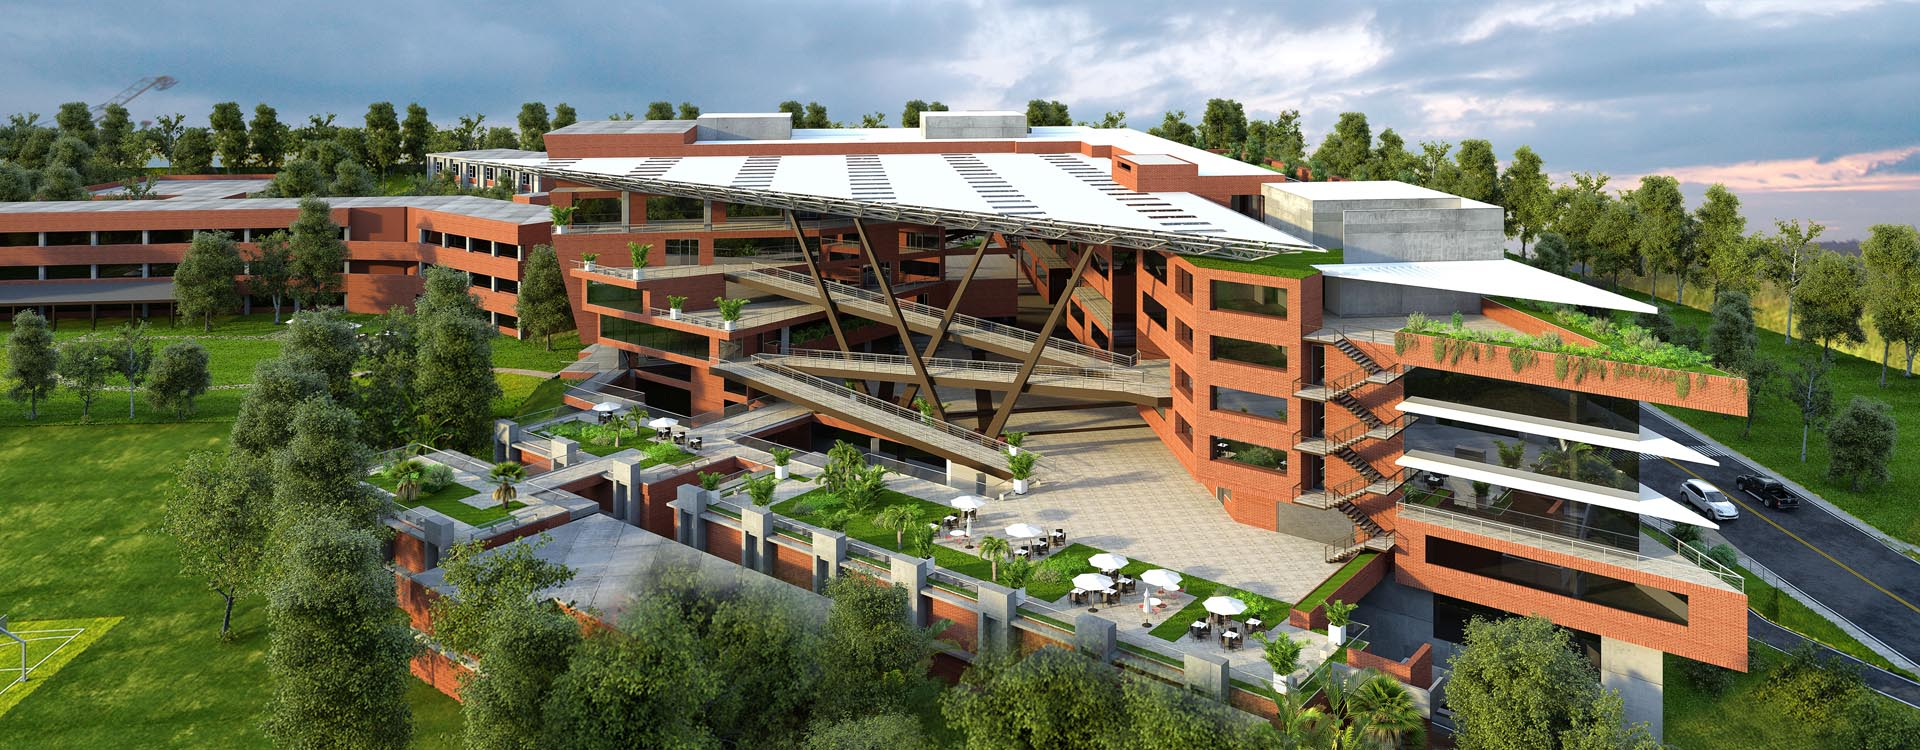
\includegraphics[height=13.25cm]{plantilla/portadacit.jpg}}
    	\makebox[\textwidth]{
    		\begin{overpic}[height=13.25cm]{\imagenportada}
     		\put(63,0){
\includegraphics[height=1.15in]{plantilla/fondologo_grande.png}}  
  			\put(64.5,2){
\includegraphics[height=0.55in]{plantilla/logoUVGblanco.eps}} 
        	\end{overpic}
    	}
    	%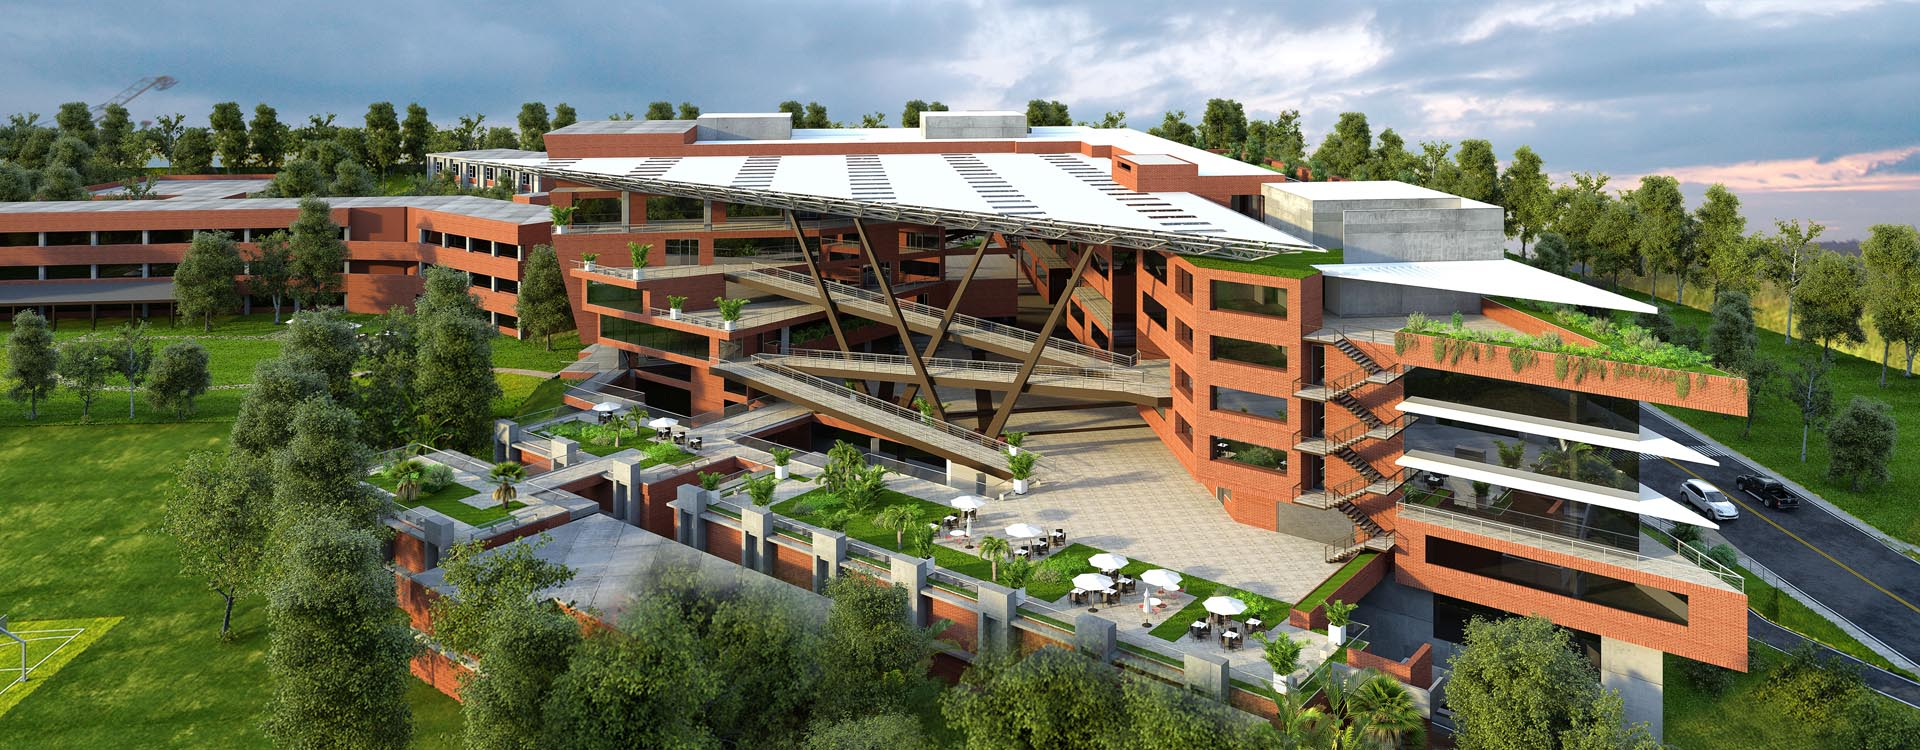
\includegraphics[height=13.25cm]{plantilla/portadacit.jpg}
	\end{figure}
	\restoregeometry
\fi

% ================================================================================
% PRIMERA PÁGINA
% ================================================================================
\ifdefined\CAPcaratula
	\newpage
%     \cleardoublepage\phantomsection
%     \pdfbookmark{Carátula}{toc}
	\pagecolor{white}
	\color{black}
	\setcounter{page}{1}
	\pagenumbering{roman}
	\thispagestyle{empty}
	\begin{center}
		\LARGE UNIVERSIDAD DEL VALLE DE GUATEMALA\\
		\LARGE Facultad de \uvgfacultad \\[0.75cm]
	\end{center}
	\begin{figure}[h]
		\begin{center}
		
\includegraphics[height=5.5 cm]{plantilla/escudoUVGnegro.eps}
		\vspace{0.5in}
		\end{center}
	\end{figure}
	\begin{center}
		\LARGE \textbf{\titulotesis} \\
		\vfill
		\vfill
		\Large Trabajo de graduación en modalidad de Tésis presentado por \\
		\Large \nombreestudiante \\
		\Large Para optar al grado académico de Licenciado en \uvgcarrera \\
		\vfill
		\large Guatemala, \mesentrega del \anoentrega
	\end{center}
\fi

% ================================================================================
% HOJA DE FIRMAS
% ================================================================================
\ifdefined\CAPfirmas
	\newpage
	\thispagestyle{empty}
	\vspace*{0.5in}
	\large Vo.Bo.:\\[1cm]
	\begin{center}
		(f) \rule[1pt]{4 in}{1pt}\\
		\nombreasesor
	\end{center}
	\vspace{1in}

	Tribunal Examinador:\\[1cm]
	\begin{center}
		(f) \rule[1pt]{4 in}{1pt}\\
		\nombreasesor \\[1in]
		(f) \rule[1pt]{4 in}{1pt}\\
		\nombreprimerex \\[1in]
		(f) \rule[1pt]{4 in}{1pt}\\
		\nombresegundoex
	\end{center}
	\vspace{1in}

	Fecha de aprobación: Guatemala, \fechaaprobacion.
	\normalsize
\fi

% ================================================================================
% CONTENIDO DEL TRABAJO
% ================================================================================
% PREFACIO
% --------------------------------------------------------------------------------
\ifdefined\CAPprefacio
	\newpage
	\cleardoublepage\phantomsection
    \chapter*{Prefacio}
    \ifdefined\parpordefecto
    	\defaultparformat{prefacio}
    \else
    	
Este trabajo surge del interés por el análisis armónico y su aplicación en el estudio de operadores pseudo-diferenciales, particularmente en contextos no euclidianos. La elección del toro $\mathbb{T}^n$ como dominio de estudio responde a su riqueza estructural como variedad compacta y grupo abeliano, lo que permite abordar problemas tanto locales como globales desde una perspectiva unificada. El texto está dirigido principalmente a estudiantes e investigadores en análisis matemático que deseen adentrarse en la teoría de operadores pseudo-diferenciales en variedades compactas. Se asumen conocimientos básicos de análisis funcional, teoría de la medida y análisis de Fourier, aunque se incluyen capítulos preliminares para facilitar la comprensión de los conceptos fundamentales. La obra se divide en tres partes claramente diferenciadas: los capítulos iniciales establecen el marco teórico necesario; la parte central desarrolla el cálculo pseudo-diferencial toroidal; y los capítulos finales presentan los principales resultados de acotación. Cada capítulo incluye la mayoría de demostraciones pertinentes, de manera que este trabajo sea lo más autocontenido posible.


La bibliografía incluye tanto referencias clásicas como contribuciones recientes, reflejando el desarrollo histórico de la teoría. Se ha puesto especial cuidado en citar trabajos fundamentales y en destacar las conexiones entre diferentes enfoques. Como resultado de este trabajo, se produjo una serie de tres artículos cientificos originales \textit{Estimates for pseudo-differential operators on the torus revisited. I, II, III}, de los cuales el primero aparecerá en el \textit{Journal of Mathematical Analysis and Applications} y los otros dos se encuentran en evaluación en otras revistas, y dos notas cortas \textit{Boundedness of pseudo-differential operators on the torus via kernel estimates} y \textit{Boundedness of toroidal pseudo-differential operators on Hardy spaces}, que apareceran en \textit{Trends in Mathematics} de la editorial \textit{Springer}, todos ellos en colaboración con el Dr. Duván Cardona. Invitamos al lector a abordar este texto como una guía para explorar un área fascinante del análisis moderno. Las demostraciones seleccionados buscan no solo transmitir resultados, sino también desarrollar la intuición matemática necesaria para futuras investigaciones en el campo.


De manera muy especial, deseo agradecer al Dr. Duván Cardona, quien fue mi asesor para este trabajo, por darme la oportunidad de trabajar con él. Me ha acompañado en mi desarrollo como profesional y mis primeros pasos en la investigación, apoyandome con todos los detalles técnicos necesarios para enriquecer mi trabajo. Más importante aún, me ha aconsejado y apoyado enriqueciendome también como persona. Además, me abrió las puerta para participar en la Comunidad Internacional de Matemáticos de Latinoamerica (ICMAM Latin America), una hermosa comunidad con quienes espero poder compartir y colaborar durante muchos años más. 

Guatemala, Octubre de 2025

Manuel Alejandro Martínez Flores
    \fi
    \addcontentsline{toc}{chapter}{Prefacio}
\fi

% AGRADECIMIENTOS
% --------------------------------------------------------------------------------
% \ifdefined\CAPagradecimientos
% 	\newpage
%     \cleardoublepage\phantomsection
% 	\chapter*{Agradecimientos}
% 	\ifdefined\parpordefecto
%     	\defaultparformat{agradecimientos}
%     \else
%     	Class aptent taciti sociosqu ad litora torquent per conubia nostra, per inceptos himenaeos. Sed vulputate, metus vel efficitur fringilla, orci ex ultricies augue, sit amet rhoncus ex purus ut massa. Nam pharetra ipsum consequat est blandit, sed commodo nunc scelerisque. Maecenas ut suscipit libero. Sed vel euismod tellus.

Proin elit tellus, finibus et metus et, vestibulum ullamcorper est. Nulla viverra nisl id libero sodales, a porttitor est congue. Maecenas semper, felis ut rhoncus cursus, leo magna convallis ligula, at vehicula neque quam at ipsum. Integer commodo mattis eros sit amet tristique. Cras eu maximus arcu. Morbi condimentum dignissim enim non hendrerit. Sed molestie erat sit amet porttitor sagittis. Maecenas porttitor tincidunt erat, ac lacinia lacus sodales faucibus.

xxxxxxx

%     \fi 
% 	\addcontentsline{toc}{chapter}{Agradecimientos}
% \fi

% ÍNDICE GENERAL
% --------------------------------------------------------------------------------
\ifdefined\CAPindice
	\newpage
    %\cleardoublepage\phantomsection
	\renewcommand{\contentsname}{Índice}
    \phantomsection
    \pdfbookmark{\contentsname}{toc}
	\tableofcontents
\fi

% LISTADO DE FIGURAS
% --------------------------------------------------------------------------------
\ifdefined\CAPfiguras
	\newpage
    \cleardoublepage\phantomsection
	\renewcommand{\listfigurename}{Lista de Figuras}
	\listoffigures
	\addcontentsline{toc}{chapter}{Lista de Figuras}
\fi

% LISTADO DE CUADROS
% --------------------------------------------------------------------------------
\ifdefined\CAPcuadros
	\newpage
    \cleardoublepage\phantomsection
	\renewcommand{\listtablename}{Lista de Cuadros}
	\listoftables
	\addcontentsline{toc}{chapter}{Lista de Cuadros}
\fi

% RESUMEN
% --------------------------------------------------------------------------------
\ifdefined\CAPresumen
	\newpage
    \cleardoublepage\phantomsection
	\chapter*{Resumen}
	\ifdefined\parpordefecto
		\defaultparformat{resumen}
	\else
		Lorem ipsum dolor sit amet, consectetur adipiscing elit. Cras vitae eleifend ipsum, ut mattis nunc. Pellentesque ac hendrerit lacus. Cras sollicitudin eget sem nec luctus. Vivamus aliquet lorem id elit venenatis pellentesque. Nam id orci iaculis, rutrum ipsum vel, porttitor magna. Etiam molestie vel elit sed suscipit. Proin dui risus, scelerisque porttitor cursus ac, tempor eget turpis. Aliquam ultricies congue ligula ac ornare. Duis id purus eu ex pharetra feugiat. Vivamus ac orci arcu. Nulla id diam quis erat rhoncus hendrerit. Class aptent taciti sociosqu ad litora torquent per conubia nostra, per inceptos himenaeos. Sed vulputate, metus vel efficitur fringilla, orci ex ultricies augue, sit amet rhoncus ex purus ut massa. Nam pharetra ipsum consequat est blandit, sed commodo nunc scelerisque. Maecenas ut suscipit libero. Sed vel euismod tellus.

Proin elit tellus, finibus et metus et, vestibulum ullamcorper est. Nulla viverra nisl id libero sodales, a porttitor est congue. Maecenas semper, felis ut rhoncus cursus, leo magna convallis ligula, at vehicula neque quam at ipsum. Integer commodo mattis eros sit amet tristique. Cras eu maximus arcu. Morbi condimentum dignissim enim non hendrerit. Sed molestie erat sit amet porttitor sagittis. Maecenas porttitor tincidunt erat, ac lacinia lacus sodales faucibus. Integer nec laoreet massa. Proin a arcu lorem. Donec at tincidunt arcu, et sodales neque. Morbi rhoncus, ligula porta lobortis faucibus, magna diam aliquet felis, nec ultrices metus turpis et libero. Integer efficitur erat dolor, quis iaculis metus dignissim eu.
	\fi
	\addcontentsline{toc}{chapter}{Resumen}
\fi

% INTRODUCCIÓN
% --------------------------------------------------------------------------------
\ifdefined\CAPintroduccion
	\newpage
	\pagenumbering{arabic}
	\setcounter{page}{1}
	\chapter{Introducción}
	\ifdefined\parpordefecto
		\defaultparformat{introduccion}
	\else
		El estudio de los operadores pseudo-diferenciales constituye una de las piedras angulares del análisis moderno, con aplicaciones profundas en la teoría de ecuaciones diferenciales parciales, el análisis armónico y la teoría espectral. Estos operadores generalizan tanto a los operadores diferenciales como a los multiplicadores de Fourier, permitiendo un tratamiento unificado de problemas que involucran no solo la regularidad de soluciones, sino también la acotación en diversos espacios funcionales. En el caso euclidiano, la teoría está bien establecida gracias a los trabajos fundacionales de Calderón, Zygmund, Hörmander y Fefferman, entre otros. Sin embargo, el estudio de estos operadores en variedades compactas, como el toro $\mathbb{T}^n := \mathbb{R}^n / \mathbb{Z}^n$, presenta desafíos particulares debido a la estructura discreta de su espacio de frecuencias y a la necesidad de desarrollar herramientas adaptadas a este contexto.

En el toro, el cálculo pseudo-diferencial puede abordarse de dos maneras: mediante una formulación local, tratando al toro como una variedad y utilizando particiones de la unidad, o mediante una definición global, aprovechando la estructura de grupo subyacente. Este trabajo se centra en este último enfoque, siguiendo el marco desarrollado por Ruzhansky, Turunen y Vainikko, que permite definir operadores pseudo-diferenciales toroidales a través de series de Fourier discretas. Esta perspectiva no solo es natural para el toro, sino que también facilita el estudio de propiedades de acotación en espacios de Lebesgue $L^p(\mathbb{T}^n)$ y de Sobolev $W^s_p(\mathbb{T}^n)$, entre otros.

Uno de los problemas centrales en la teoría es determinar bajo qué condiciones un operador pseudo-diferencial $T_a$, definido por un símbolo $a(x, \xi)$ en una clase de Hörmander $S^m_{\rho,\delta}(\mathbb{T}^n \times \mathbb{Z}^n)$, se extiende a un operador acotado entre espacios de funciones. Resultados clásicos, como los de Calderón-Vaillancourt para $L^2(\mathbb{R}^n)$ o los de Fefferman para $L^p(\mathbb{R}^n)$, han establecido cotas que dependen críticamente de los parámetros $m, \rho, \delta$ del símbolo. En el caso toroidal, aunque muchos de estos resultados tienen análogos, las demostraciones requieren ajustes sustanciales debido a la naturaleza discreta del espacio de frecuencias $\mathbb{Z}^n$ y a la falta de invarianza bajo cambios de coordenadas cuando $\rho > 1 - \delta$.

Este trabajo tiene como objetivo revisar y exponer de manera sistemática los resultados de continuidad de operadores pseudo-diferenciales en el toro, haciendo especial hincapié en las técnicas de demostración y en las diferencias con el caso euclidiano. Se abordarán tanto resultados clásicos como contribuciones recientes, incluyendo los teoremas de Delgado para $L^p(\mathbb{T}^n)$ con $p \geq 2$ y las extensiones de Álvarez-Hounie realizadas con Cardona para el rango completo $1 < p < \infty$. 

La exposición se estructura en tres capítulos principales. Inicialmente, se presentan los preliminares necesarios sobre espacios de funciones, transformadas de Fourier y distribuciones en $\mathbb{R}^n$ y $\mathbb{T}^n$. Además, se incluyen resultados clásicos de análisis armónico, como el hecho que el espacio $\mathrm{BMO}$ es el dual del espacio de Hardy $H^1$ y técnicas de interpolación compleja que permiten extender propiedades de continuidad a espacios $L^p$ con $1 < p < \infty$. Luego, se introduce la definición y propiedades básicas de los operadores pseudo-diferenciales en ambos contextos, destacando las particularidades del cálculo toroidal, como el uso de operadores de diferencia discreta en lugar de derivadas convencionales. Finalmente, se dedican dos capítulos a demostrar los principales resultados de continuidad en espacios de Lebesgue y de Sobolev, utilizando técnicas que incluyen interpolación, descomposiciones atómicas y estimaciones de núcleos integrales.

Cabe destacar que, a diferencia del caso euclidiano, las clases $H^1$ y $\mathrm{BMO}$ no son estables bajo la multiplicación de funciones test en el toro, lo que imposibilita tratar este espacio simplemente como una variedad mediante particiones de la unidad. Esta limitación justifica el estudio independiente del caso toroidal y la necesidad de desarrollar herramientas específicas para este contexto. Asimismo, los operadores pseudo-diferenciales con símbolos en las clases de Hörmander no son estables bajo cambios de coordenadas cuando $\rho > 1 - \delta$, lo que refuerza la relevancia de un tratamiento global mediante la transformada de Fourier discreta.

Con este trabajo, se espera proporcionar una referencia accesible y rigurosa que contribuya a la divulgación de estos temas en español y fomente futuras investigaciones en el área. La escasez de literatura en español sobre operadores pseudo-diferenciales representa una barrera significativa para estudiantes e investigadores hispanohablantes, limitando su acceso a herramientas avanzadas y reduciendo las oportunidades de formación especializada. Esta exposición busca reducir esta brecha, permitiendo el acceso a conceptos avanzados y contribuyendo a fortalecer la comunidad matemática en español.
	\fi
\fi

% OBJETIVOS
% --------------------------------------------------------------------------------
\ifdefined\CAPobjetivos
	\newpage
	\chapter{Objetivos}
	\ifdefined\parpordefecto
		\defaultparformat{objetivos}
	\else
		\section{Objetivo General}
Revisar y exponer los conceptos fundamentales en el estudio de operadores pseudo-diferenciales, detallando teoremas y demostraciones importantes para su entendimiento e investigación.

\section{Objetivos Específicos}
\begin{itemize}
    \item Definir y explicar los conceptos clave para el estudio de operadores pseudo-diferenciales
    \item Desarrollar con rigor matemático las bases teóricas de los operadores pseudo-diferenciales
    \item Introducir de forma accesible al estado del arte en la investigación de operadores pseudo-diferenciales
\end{itemize}
	\fi
\fi

% JUSTIFICACIÓN
% --------------------------------------------------------------------------------
\ifdefined\CAPjustificacion
	\newpage
	\chapter{Justificación}
	\ifdefined\parpordefecto
		\defaultparformat{justificacion}
	\else
		El estudio de los operadores pseudo-diferenciales es esencial en el análisis moderno, con aplicaciones clave en ecuaciones diferenciales parciales (EDP), análisis armónico y teoría espectral. Sin embargo, la falta de recursos en español sobre el tema representa una barrera significativa para estudiantes e investigadores hispanohablantes, limitando su acceso a herramientas avanzadas y reduciendo las oportunidades de formación especializada. Esta carencia no solo dificulta el aprendizaje autónomo, sino que también desincentiva la investigación en áreas teóricas y aplicadas donde estos operadores son fundamentales, como el análisis de regularidad de soluciones de EDP's. Este trabajo busca reducir esta brecha, proporcionando una exposición clara y rigurosa de los operadores pseudo-diferenciales en el toro y sus propiedades de continuidad. Permitiendo así, el acceso a conceptos avanzados y contribuyendo a fortalecer la comunidad matemática en español, promoviendo la investigación y la innovación en un campo con amplias proyecciones teóricas y aplicadas.

	\fi
\fi

% MARCO TEÓRICO
% --------------------------------------------------------------------------------
\ifdefined\CAPmarcoteorico
	\newpage
	\chapter{Marco Teórico}
	\ifdefined\parpordefecto
		\defaultparformat{marco_teorico}
	\else
		\input{marco_teorico}
	\fi
\fi

% ANTECEDENTES
% --------------------------------------------------------------------------------
\ifdefined\CAPantecedentes
	\newpage
	\chapter{Antecedentes}
	\ifdefined\parpordefecto
    	\defaultparformat{antecedentes}
    \else
    	En el caso euclidiano, Calderón y Vaillancourt demostraron que los operadores pseudo-diferenciales con símbolos en la clase $S^{0}_{\rho,\rho}(\mathbb{R}^n\times\mathbb{R}^n)$ son acotados en $L^2(\mathbb{R}^n)$ para algún $0\leq\rho<1$, véase \cite{calderon-vaillancourt-1, calderon-vaillancourt-2}. Este resultado no puede extenderse cuando $\rho=1$, es decir, existen símbolos en $S^{0}_{1,1}(\mathbb{R}^n\times\mathbb{R}^n)$ cuyos operadores pseudo-diferenciales asociados no son acotados en $L^2$; para un argumento clásico de este hecho debido a Hörmander, consúltese \cite{duoandikoetxea}. Además, Fefferman \cite{fefferman-Lp} probó la acotación $L^\infty(\mathbb{R}^n)$-$\mathrm{BMO}(\mathbb{R}^n)$ para operadores pseudo-diferenciales con símbolos en la clase $S^{m}_{\rho,\delta}(\mathbb{R}^n\times\mathbb{R}^n)$, con $m=-n(1-\rho)/2$ donde $0\leq \delta<\rho\leq 1$. Fefferman también obtuvo la acotación en $L^p(\mathbb{R}^n)$ para estas clases cuando $m\leq -n(1-\rho)|1/p - 1/2|$ y $1<p<\infty$. En vista de ejemplos clásicos debidos a Wainger y Hirschman, el resultado de Fefferman es óptimo para multiplicadores de Fourier. Cabe destacar que el desarrollo histórico del problema de la acotación en $L^p$ de operadores pseudo-diferenciales ha sido discutido en $\mathbb{R}^n$, por ejemplo, en \cite{nagase, wang}.  

Los operadores pseudo-diferenciales con símbolos en las clases de Hörmander pueden definirse en variedades $C^\infty$ mediante cartas locales. Por ello, se considera el toro $\mathbb{T}^n:=\mathbb{R}^n/\mathbb{Z}^n$ como un grupo aditivo cociente y una $n$-variedad, con el atlas preferido de sistemas de coordenadas dado por la aplicación de restricción $x\mapsto x + \mathbb{Z}^n$ en conjuntos abiertos $\Omega \subset \mathbb{R}^n$, véase McLane \cite{mclane}. Se nota que en \cite{agranovich}, Agranovich proporciona una definición global de operadores pseudo-diferenciales en el círculo $\mathbb{S}^1=\mathbb{T}^1$, en lugar de la formulación local que trata al círculo como una variedad. Mediante la transformada de Fourier, esta definición se extendió al toro $\mathbb{T}^n$. Además, se ha demostrado que las clases $(\rho,\delta)$ de Agranovich y Hörmander son equivalentes, gracias al teorema de equivalencia de McLane \cite{mclane}. En este trabajo, se consideran operadores pseudo-diferenciales toroidales en el contexto del cálculo pseudo-diferencial en el toro desarrollado por Ruzhansky, Turunen y Vainniko \cite{ruzhansky-turunen2, ruzhansky-turunen}. Asimismo, cotas $L^p$ en el círculo que pueden extenderse al toro se encuentran en \cite{wong}, en el marco clásico de la teoría de Calderón-Zygmund. Por otro lado, el análogo toroidal del resultado de Fefferman fue probado por Delgado en \cite{delgado} para el toro, aunque aún se requiere que $\delta<\rho$.   
Se nota que, para $0\leq \delta<1$ y $0<\rho\leq 1$, Álvarez y Hounie \cite{alvarez-hounie} probaron la acotación $L^p(\mathbb{R}^n)$-$L^q(\mathbb{R}^n)$ de operadores pseudo-diferenciales cuando $p\leq q$, incluso con $\delta \geq \rho$. Este resultado fue extendido al caso toroidal en \cite{Cardona:Martinez}. 
Para otros trabajos sobre acotación $L^p$ de operadores pseudo-diferenciales, se remite al lector a \cite{cardona, molahajloo-wong, ruzhansky-turunen-quant}.
    \fi  
\fi

% ALCANCE
% --------------------------------------------------------------------------------
\ifdefined\CAPalcance
	\newpage
	\chapter{Alcance}
	\ifdefined\parpordefecto
    	\defaultparformat{alcance}
    \else
    	Podemos usar \Gls{latex} para escribir de forma ordenada una \gls{formula} matemática. 
    \fi 
\fi

% CAPÍTULOS
% --------------------------------------------------------------------------------
\newpage
\ifdefined\parpordefecto
	\defaultparformat{capitulos}
\else
	\chapter{Preliminares}

En este capítulo se revisarán aspectos básicos del análisis armónico en 
$\R^n$ y $\T^n$. 
Se recuerda que $\R^n$ es un grupo aditivo respecto a la suma usual de vectores
con subgrupo aditivo $\Z^n$. Entonces, se define al toro $n$-dimensional
como el grupo cociente $\T^n := \R^n/\Z^n = (\R/\Z)^n$. Además, 
el toro puede ser identificado con el conjunto $[0, 1)^n$ y se le puede considerar
con la topología cociente. A lo largo de este trabajo, se fijará la
medida de Lebesgue en $\R^n$. Para cualquier punto 
$x := (x_1, \ldots, x_n) \in \R^n$, se denotará la norma
euclideana como 
\begin{equation*}
    |x| := \sqrt{x_1^2 + \cdot + x_n^2}.
\end{equation*}
Sin embargo, podría ser problemático considerar potencias negativas
de la norma euclideana, debido a que se desvanece en cero. Por lo que
se considerará una función que se comporta asintóticamente similar, 
pero no presenta el mismo problema
\begin{equation*}
    \angles{x} := \sqrt{1 + |x|^2}.
\end{equation*}
Si se tiene que existe una constante $C>0$ tal que $A\leq CB$, se dice que $A\lesssim B$. Si además, $C$ depende de algún parámetro $\alpha$, se denota $A\lesssim_\alpha B$.
\section{Espacios de Lebesgue en $\R^n$ y $\T^n$ }

Sea $\Omega$ un subconjunto medible de $\R^n$. Por simplicidad, se supondrá
que $\Omega$ es abierto o cerrado.

\begin{definition}
    Dado $1\leq p < \infty$. Se dice que una función medible $f:\Omega\subset\R^n\rightarrow\C$ se encuentra en $L^p(\Omega)$ si su norma 
    \begin{equation*}
        \|f\|_{L^p(\Omega)} := \left( \int_\Omega |f(x)|^p \diff x
        \right)^{1/p}
    \end{equation*}
    es finita. Para el caso $p=\infty$, se dice que $f\in L^\infty(\Omega)$
    si es esencialmente acotada. Es decir, si
    \begin{equation*}
        \|f\|_{L^\infty(\Omega)} := \esssup_{x\in\Omega}|f(x)| < \infty,
    \end{equation*}
    donde $\esssup_{x\in\Omega}|f(x)|$ se define como el menor número real $M$
    tal que es mayor que $|f(x)|$ casi para todo $x\in\Omega$, i.e. excepto fuera de
    un conjunto de medida cero.
\end{definition}
Cabe destacar que en realidad los elementos de los espacios $L^p(\Omega)$
son clases de equivalencias de funciones iguales casi en todo $x\in\Omega$.
Sin embargo, es un detalle técnico menor y se acostumbra a tratarles como funciones.
Además, cuando $\Omega$ sea claro por el contexto, simplemente se denotará
$\|\cdot\|_{L^p(\Omega)}$ como $\|\cdot\|_{L^p}$. Ahora, se discutirán propiedades 
importantes de los espacios de Lebesgue.

\begin{proposition}[Desigualdad de Young]
    Sean $1< p, q< \infty$, tales que $\frac{1}{p} + \frac{1}{q} = 1$.
    Entonces para todos $a, b > 0$, se tiene que 
    \begin{equation*}
        ab \leq \frac{a^p}{p} + \frac{b^q}{q}.
    \end{equation*}
    Como consecuencia, para $f\in L^p(\Omega)$ y $g \in L^q(\Omega)$,
    se tiene que $fg \in L^1(\Omega)$ y 
    \begin{equation*}
        \|fg\|_{L^1} \leq \frac{1}{p}\|f\|^p_{L^p} + \frac{1}{q}
        \|g\|_{L^q}^q.
    \end{equation*}
\end{proposition}
\begin{proof}
    Esto es consecuencia del hecho que $x\mapsto e^x$ es una función
    convexa. Entonces
    \begin{equation*}
        ab = e^{\ln a + \ln b} = e^{\frac{1}{p}\ln a^p + 
        \frac{1}{q}\ln b^q} \leq \frac{1}{p}e^{\ln a^p} +
        \frac{1}{q}e^{\ln b^q} = \frac{a^p}{p} + \frac{b^q}{q}.
    \end{equation*}
    Completando así la prueba.
\end{proof}
Particularmente cuando $p=2=q$, se tiene la conocida como desigualdad de
Cauchy. 
\begin{proposition}[Desigualdad de H\"older]
    Sean $1\leq p, q\leq \infty$, tales que $\frac{1}{p} + \frac{1}{q} = 1$.
    Entonces, para $f\in L^p(\Omega)$ y $g\in L^p(\Omega)$, se tiene
    que $fg \in L^1(\Omega)$ y 
    \begin{equation*}
        \|fg\|_{L^1} \leq \|f\|_{L^p}\|g\|_
        {L^q}.
    \end{equation*}
\end{proposition}
\begin{proof}
    Para el caso $p=1$ o $p=\infty$, el resultado es trivial. Así que 
    se considerará el caso $1<p<\infty$, que es una aplicación 
    de la proposición anterior. Primero, se supone
    que $\|f\|_{L^p} = \|g\|_{L^q} = 1$. Entonces, 
    se tiene que
    \begin{equation*}
        \|fg\|_{L^1} \leq \frac{1}{p}\|f\|_{L^p} + \frac{1}{q}\|g\|_{L^q} 
        = 1.
    \end{equation*}
    Ahora, se nota que si $\|f\|_{L^p}$ o $\|g\|_{L^q}$ se anulan, 
    entonces se trivializa la desigualdad. 
    Por lo que se puede considerar el caso más general en el que ninguna de las
    normas se anula de la siguiente manera
    \begin{equation*}
        \left\| \frac{f}{\|f\|_{L^p}} \frac{g}{\|g\|_{L^q}}
        \right\|_{L^1} \leq 1.
    \end{equation*}
    El resultado sigue de la linealidad de la norma $L^1$.
\end{proof}
En el caso $p=2=q$ se obtiene la desigualdad de Cauchy-Schwarz.

\begin{proposition}[Desigualdad de Minkowski]
    Dado $1\leq p\leq\infty$, sean $f,g\in L^p(\Omega)$. Entonces se tiene que
    \begin{equation*}
        \|f+g\|_{L^p} \leq \|f\|_{L^p} +
        \|g\|_{L^p}.
    \end{equation*}
    Particularmente, $\|\cdot\|_{L^p}$ satisface la desigualdad triangular
    y $L^p(\Omega)$ es un espacio normado.
\end{proposition}
\begin{proof}
    Para $p=1$ o $p=\infty$ el resultado se obtiene gracias a la desigualdad
    triangular del módulo en los números complejos. Ahora, para $1<p<\infty$ 
    se tiene que
    \begin{align*}
        \|f+g\|_{L^p}^p & \leq \int_\Omega |f+g|^{p-1}(|f|+|g|)\diff x\\
        & = \int_\Omega |f+g|^{p-1}|f| \diff x + 
        \int_\Omega |f+g|^{p-1}|g| \diff x \\
        & \leq \left( 
            \int_\Omega |f+g|^{(p-1) \frac{p}{p-1}} \diff x 
        \right)^{\frac{p-1}{p}} \left[
            \left(\int_\Omega |f|^p\diff x\right)^{1/p} +
            \left(\int_\Omega |g|^p\diff x\right)^{1/p}
        \right] \\ 
        & = \|f+g\|_{L^p}^{p-1}(\|f\|_{L^p} + \|g\|_{L^p}).
    \end{align*}
    Aquí, la primera desigualdad es la desigualdad triangular de los números
    complejos y la segunda es la desigualdad de H\"older, por lo que se concluye
    lo deseado.
\end{proof}

Ahora se introducen dos resultados importantes y de bastante utilidad. Sin embargo,
sus demostraciones requieren de herramientas de teoría de la medida o del 
análisis complejo que se encuentran fuera del alcance de este trabajo. Por lo que
simplemente se enuncian y se recomienda al lector investigar los detalles.

\begin{proposition}[Monotonía de la norma $L^p$]\label{prop:monotonia-Lp}
    Sea $f:\Omega_1 \times \Omega_2 \subset\R^n\times\R^n\rightarrow\C$ y 
    sea $1\leq p\leq\infty$.
    Se supone que $f(\cdot,y)\in L^p(\Omega_1)$ para casi
    todo $y$, y que $y\mapsto \|f(\cdot, y)\|_{L^p}$ se encuentra en
    $L^1(\Omega_2)$. Entonces $f(x, \cdot)\in L^1(\Omega_2)$ para casi
    todo $x$, la función $x\mapsto \int_{\Omega_2} f(x, y)\diff y$ se encuentra
    en $L^p(\Omega_1)$, y
    \begin{equation*}
        \left\| \int_{\Omega_2} f(\cdot, y)\diff y
        \right\|_{L^p(\Omega_1)} \leq \int_{\Omega_2} 
        \|f(\cdot, y)\|_{L^p(\Omega_1)} \diff y.
    \end{equation*}
\end{proposition}
A continuación se presenta un resultado clásico de la interpolación de 
operadores y espacios de
funciones. Para una discusión más profunda de estas técnicas, se recomienda 
revisar Bergh y L\"ofstrom \cite{bergh-lofstrom}.
\begin{theorem}[Interpolación de Riesz-Thorin]\label{theo:riesz-thorin} 
    Sea $T:L^{p_0}(\Omega)+L^{p_1}(\Omega) \rightarrow 
    L^{q_0}(\Omega)+L^{q_1}(\Omega)$ un operador lineal tal que 
    \begin{equation*}
        \|Tf\|_{L^{q_0}} \leq M_0 \|f\|_{L^{p_0}}, \quad
        \|Tf\|_{L^{q_1}} \leq M_1 \|f\|_{L^{p_1}}.
    \end{equation*}
    Para cualquier $0<\theta<1$, se definen 
    \begin{equation*}
        \frac{1}{p_\theta} = \frac{1-\theta}{p_0} + \frac{\theta}{p_1}, 
        \quad 
        \frac{1}{q_\theta} = \frac{1-\theta}{q_0} + \frac{\theta}{q_1}.
    \end{equation*}
    Entonces, $T$ extiende a un operador continuo de $L^{p_\theta}(\Omega)$
    en $L^{q_\theta}(\Omega)$. Además, 
    \begin{equation*}
        \|Tf\|_{L^{q_\theta}} \leq M_0^{1-\theta}M_1^\theta \|f\|_{L^{p_\theta}}.
    \end{equation*}
\end{theorem}
Se continúa con el programa de definiciones y propiedades en los espacios 
de Lebesgue.

\begin{definition}[Convoluciones]
    Para funciones $f,g\in L^1(\R^n)$ se define su convolución como 
    \begin{equation*}
        (f*g)(x) := \int_{\R^n} f(x-y)g(y)\diff y.
    \end{equation*}
    Se puede notar que el cambio de variable $y\mapsto x-u$ implica la
    conmutatividad, es decir $f*g=g*f$.
\end{definition}
\begin{remark}
    En la definición anterior existe la pregunta sobre la convergencia de la
    integral. Para definir la convolución de forma rigurosa, se podría definir 
    primero para funciones que cumplan condiciones de regularidad más 
    fuertes, como las del espacio de Schwartz que se definirá en la siguiente
    sección, para luego definir el operador $*:L^1\times L^1 \rightarrow L^1$
    que estaría bien definido gracias a la siguiente propiedad.
\end{remark}

\begin{proposition}[Desigualdad de Young para convoluciones]
    Sean $1\leq p,q,r\leq \infty$ tales que $\frac{1}{p} + \frac{1}{q} = 1 + 
    \frac{1}{r}$, y sean $f \in L^p(\R^n)$, $g\in L^q(\R^n)$. Entonces
    se tiene que
    \begin{equation*}
        \|f*g\|_{L^r} \leq \|f\|_{L^p} \|g\|_{L^q}.
    \end{equation*}
\end{proposition}
\begin{proof}
    Se nota que gracias al teorema~\ref{theo:riesz-thorin} es suficiente 
    demostrar 
    \begin{equation}\label{eq:young-convolution-estimates}
        \|f*g\|_{L^p} \leq \|f\|_{L^p} \|g\|_{L^1}, \quad 
        \|f*g\|_{L^\infty} \leq \|f\|_{L^p} \|g\|_{L^t},
    \end{equation}
    para $\frac{1}{t} + \frac{1}{p} = 1$. En efecto, bastaría con considerar 
    el operador $f * \cdot$, los parametros
    \begin{equation*}
        p_0 = 1, \quad p_1 = t, \quad q_0 = p, \quad q_1 = \infty.
    \end{equation*}
    y $\|f\|_{L^p}$ como ambas constantes de estimación.
    Al aplicar la interpolación
    \begin{equation*}
        \frac{1}{r} = \frac{1-\theta}{p} + \frac{\theta}{\infty}, \quad 
        \frac{1}{q} = \frac{1-\theta}{1} + \frac{\theta}{t},
    \end{equation*}
    se obtiene la condición indicada para los parametros $p, q, r$. Ahora, 
    se procede a demostrar el primer estimativo de
    ~(\ref{eq:young-convolution-estimates}). Este se obtiene como resultado de
    la monotonia de la norma $L^p$, véase la proposición~\ref{prop:monotonia-Lp}.
    En efecto,
    \begin{align*}
        \|f*g\|_{L^p} & = \left\| \int_{\R^n} f(\cdot-y)g(y)\diff y 
        \right\|_{L^p} \\
        & \leq \int_{\R^n} \|f(\cdot-y)\|_{L^p} |g(y)|\diff y \\
        & \leq \|f\|_{L^p}\|g\|_{L^1}.
    \end{align*}
    Por otra parte, el segundo estimativo es resultado de la desigualdad de 
    H\"older 
    \begin{align*}
        \|f*g\|_{L^\infty} & \leq \int_{\R^n} |f(x-y)||g(y)| \diff y \\
        & \leq \|f\|_{L^p}\|g\|_{L^t}.
    \end{align*}
    Concluyendo con el resultado deseado.
\end{proof}
Se continua con un resultado importante sobre convergencia en 
espacios $L^p$
\begin{theorem}[Convergencia dominanda de Lebesgue]
    Sea $(f_k)_{k=1}^\infty$ una secuencia de funciones medibles en $\Omega$ 
    tales que convergen puntualmente a $f$ para casi todo $x\in\Omega$. Se supone
    que existe $g\in L^1(\Omega)$ tal que $|f_k|\leq g$ para todo $k$. Entonces
    $f$ es integrable y 
    \begin{equation*}
        \int_\Omega f \diff x = \lim_{k\rightarrow\infty} \int_\Omega 
        f_k \diff x.
    \end{equation*}
\end{theorem}

\begin{remark}
    Una implicación del resultado anterior es el hecho que los espacios $L^p$ son 
    completos, y por consecuencia son espacios de Banach. Particularmente, el 
    espacio $L^2$ es un espacio de Hilbert con producto interno dado por
    \begin{equation*}
        \angles{f, g}_{L^2} := \int_\Omega f\overline{g}\diff x,
    \end{equation*}
    donde $\overline{z}$ es el conjugado en los números complejos.
\end{remark}
Se concluye esta sección con la definición de la versión local de los espacios de Lebesgue. Para ello se necesita el siguiente espacio de funciones.
\begin{definition}[Funciones suaves de soporte compacto]
		Se dice que $\varphi:\Omega\subset\R^n\rightarrow\C$ es suave si es de clase $C^\infty$, o infinitamente diferenciable.  Se define su soporte como 
		\begin{equation*}
			\supp \varphi = \overline{\{x\in\Omega:\varphi(x)\neq 0\}}.
		\end{equation*}
		Si $\supp \varphi$ es compacto, se dice que $f\in\C^\infty_0(\Omega)$.
\end{definition}
\begin{definition}[Localización de espacios de Lebesgue]
	Se dice que una función medible $f:\Omega\subset\R^n\rightarrow\C$ es localmente integrable o pertenece a $L^{p}_{loc}(\Omega)$, con $1\leq p\leq\infty$ si 
	\begin{equation*}
		\|f\varphi\|_{L^p} < \infty,
	\end{equation*} 
	para todo $\varphi\in C^\infty_0(\Omega)$.
\end{definition}
\section{Transformada de Fourier en $\R^n$}
Ahora, se procede a definir y mostrar propiedades importantes de la
transformada de Fourier, una herramienta fundamental para el estudio
de las ecuaciones diferenciales en general y los operadores
pseudo-diferenciales en particular. 

\begin{definition}[Transformada de Fourier en $\R^n$]
    Dada $f\in L^1(\R^n)$, se define su transformada de Fourier como 
    \begin{equation*}
        (\mathcal{F}_{\R^n}f)(\xi) = \widehat{f}(\xi) := \int_{\R^n}
        e^{-2\pi i x \cdot \xi} f(x) \diff x,
    \end{equation*}
    para cualquier $\xi \in \R^n$.
\end{definition}

\begin{proposition}
    La transformada de Fourier es un operador continuo 
    $\mathcal{F}_{\R^n} : L^1(\R^n) \rightarrow L^\infty(\R^n)$ con norma uno:
    \begin{equation*}
        \|\widehat{f}\|_{L^\infty} \leq \|f\|_{L^1}.
    \end{equation*}
    Además, $\widehat{f}$ es continua en todas partes. 
\end{proposition}
\begin{proof}
    El estimativo es resultado de la desigualdad de Minkowski para integrales
    clásica 
    \begin{align*}
        \left|
            \int_{\R^n} e^{-2\pi i x \cdot \xi} f(x) \diff x
        \right| & \leq 
        \int_{\R^n} \left|e^{-2\pi i x \cdot \xi}\right|| f(x)| \diff x\\
        & \leq \|f\|_{L^1}.
    \end{align*}
    Ahora, la continuidad es consecuencia del teorema de convergencia dominada
    de Lebesgue. Para cualquier $\xi_k \rightarrow \xi$ se define 
    \begin{equation*}
        h_k(x) :=  e^{-2\pi i x \cdot \xi_k} f(x)
    \end{equation*}
    Entonces, se tiene que $|h_k| \leq |f|$ y se obtiene que 
    \begin{equation*}
        \int_{\R^n} e^{-2\pi i x \cdot \xi} f(x) \diff x = 
        \lim_{k\rightarrow\infty}\int_{\R^n} e^{-2\pi i x \cdot \xi_k} f(x) \diff x.
    \end{equation*} 
    Que es exactamente $\widehat{f}(\xi) = \lim \widehat{f}(\xi_k)$, el 
    resultado deseado.
\end{proof}
A pesar de que la transformada de Fourier está bien definida en el espacio
$L^1(\R^n)$, este presenta ciertas limitaciones técnicas debido a los pocos
requerimientos de regularidad para las funciones en este espacio. Es muy útil
tener acceso a otras herramientas resultantes de continuidad, diferenciabilidad,
y decaimiento.
Por lo tanto, se introduce notación que será importante a lo largo de este trabajo. 
\begin{definition}[Notación de multi-índice]
    Para $\alpha:=(\alpha_1, \ldots, \alpha_n), \beta:=(\beta_1, \ldots, \beta_n) 
    \in \N_0^n$, se define 
    \begin{equation*}
        \partial^\alpha := \frac{\partial^{\alpha_1}}{\partial x_1^{\alpha_1}}
        \cdots \frac{\partial^{\alpha_n}}{\partial x_n^{\alpha_n}}.
    \end{equation*}
    De forma similar, $x^\beta := x_1^{\beta_1} \cdots x_n^{\beta_n}$. Se dice 
    que $\alpha \leq \beta$ si $\alpha_i \leq \beta_i$ para todo $i$. Además, 
    se denota la longitud del multi-índice como
    $|\alpha| := \alpha_1 + \cdots \alpha_n$ y su factorial como
    $\alpha! := \alpha_1! \cdots \alpha_n!$.
\end{definition}

\begin{definition}[Espacio de Schwartz $\mathcal{S}(\R^n)$]
    Se dice que una función suave (infinitamente diferenciable) 
    $\varphi:\R^n\rightarrow\C$ se encuentra en $\mathcal{S}(\R^n)$ si se 
    cumple que
    \begin{equation*}
        \sup_{x\in\R^n}|x^\beta \partial^\alpha \varphi(x)| < \infty, 
    \end{equation*}
    para cualesquiera multi-índices $\alpha, \beta \in \N_0^n$. Ahora,
    se dice que $\varphi_j\rightarrow\varphi$ en $\mathcal{S}(\R^n)$ si
    \begin{equation*}
        \sup_{x\in\R^n}|x^\beta \partial^\alpha (\varphi_j-
        \varphi)(x)| \rightarrow 0, 
    \end{equation*}
    cuando $j\rightarrow\infty$ para cualesquiera multi-índices 
    $\alpha, \beta \in \N_0^n$.
\end{definition}
\begin{proposition}
    Para cualquier $1\leq p\leq\infty$ se tiene que 
    $\mathcal{S}(\R^n)\subset L^p(\R^n)$ con encaje continuo.
\end{proposition}
\begin{proof}
    El caso $p=\infty$ es trivial, pues las funciones en el espacio de Schwartz
    son acotadas por definición.
    Sea $\varphi_j\rightarrow0$ en $\mathcal{S}(\R^n)$, entonces
    \begin{align*}
        \int_{\R^n} |\varphi_j(x)|^p \diff x & = 
        \int_{\R^n} \angles{x}^{pN} |\varphi_j(x)|^p \angles{x}^{-pN} \diff x \\ 
        & \lesssim \max_{|\beta|\leq N} \sup_{x\in\R^n} 
        |x^\beta\varphi_j(x)|^p \int_{\R^n}\angles{x}^{-pN} \diff x \\
        & \rightarrow 0,
    \end{align*}
    donde $N\in\N$ se escoge de manera que la última integral converga. 
\end{proof}

\begin{theorem}
    Sea $\varphi\in\mathcal{S}(\R^n)$. Entonces $2\pi i\xi_j\widehat{\varphi}(\xi)
    = \widehat{\partial_j\varphi}(\xi)$ y 
    $ 2\pi i \widehat{x_j\varphi}(\xi) = - \partial_j\widehat{\varphi}(\xi)$
\end{theorem}
\begin{proof}
    Para la primera expresión se procede por integración por partes
    \begin{align*}
        \widehat{\partial_j\varphi}(\xi) & = \int_{\R^n} e^{-2\pi i x\cdot \xi} 
        \partial_{x_j}\varphi(x) \diff x \\
        & = - \int_{\R^n} (\partial_{\xi_j} e^{-2\pi i x\cdot \xi}) 
        \varphi(x) \diff x\\
        & = 2\pi i \xi_j \int_{\R^n} e^{-2\pi i x\cdot \xi} 
        \varphi(x) \diff x.
    \end{align*}
    Se nota que no aparece el término con la frontera debido a que $\varphi$ 
    se desvanece en el infinito. Ahora, para la segunda expresión 
    \begin{equation*}
        \partial_{\xi_j} \widehat{\varphi}(\xi) = 
        \int_{\R^n}  e^{-2\pi i x\cdot \xi} (-2\pi i x_j)
        \varphi(x) \diff x.
    \end{equation*}
    Concluyendo la prueba.
\end{proof}
Por lo que se puede concluir lo siguiente 
\begin{corollary}
    Sea $\varphi\in\mathcal{S}(\R^n)$. Entonces, 
    \begin{equation*}
        \xi^\beta \partial^\alpha \widehat{\varphi}(\xi) = 
        (2\pi i)^{|\alpha|-|\beta|} (-1)^{|\alpha|} \widehat{\partial^\beta 
        [x^\alpha \varphi]}(\xi).
    \end{equation*}
    Por lo que 
    \begin{align*}
        |\xi^\beta \partial^\alpha \widehat{\varphi}(\xi)| & \leq 
        |2\pi i|^{|\alpha|-|\beta|} \int_{\R^n} |\partial^\beta 
        [x^\alpha \varphi(x)]| \diff x \\
        & \leq |2\pi i|^{|\alpha|-|\beta|} \sup_{x\in\R^n} 
        \left|(1+|x|)^{n+1} \partial^\beta 
        [x^\alpha \varphi(x)]\right| \int_{\R^n} (1+|x|)^{-n-1}\diff x \\
        & = C \sup_{x\in\R^n} \left|(1+|x|)^{n+1} \partial^\beta 
        [x^\alpha \varphi(x)]\right| \\
        & < \infty.
    \end{align*}
    Particularmente, $\mathcal{F}_{\R^n}$ mapea $\mathcal{S}(\R^n)$ en sí 
    mismo. Además, por el teorema de convergencia dominada de Lebesgue, 
    la transformada de Fourier es un operador continuo.
\end{corollary}
En realidad, es un isomorfismo en $\mathcal{S}(\R^n)$. Para ello se demostrarán 
algunos lemas útiles.

\begin{lemma}[Fórmula de multiplicación para la transformada de Fourier]
    Sean $f, g \in L^1(\R^n)$. Entonces, $\int_{\R^n}\widehat{f} g \diff x 
    = \int_{\R^n} f \widehat{g} \diff x$.
\end{lemma}
\begin{proof}
    Aplicando el teorema de Fubini 
    \begin{align*}
        \int_{\R^n}\widehat{f} g \diff x & = \int_{\R^n} \left[
            \int_{\R^n} e^{-2\pi i x\cdot y} f(y) \diff y
        \right] g(x) \diff x \\
        & = \int_{\R^n} \left[
            \int_{\R^n} e^{-2\pi i x\cdot y} g(x) \diff x
        \right] f(y) \diff y \\ 
        & = \int_{\R^n} f \widehat{g} \diff y
    \end{align*}
    Concluyendo la prueba.
\end{proof}
\begin{lemma}[Transformada de Fourier para Gaussiana]
    Se tiene que
    \begin{equation*}
       \int_{\R^n} e^{-2\pi i x \cdot \xi} e^{-\varepsilon\pi^2|x|^2}
        \diff x = (\pi\varepsilon)^{-n/2} e^{-|\xi|^2/\varepsilon},  
    \end{equation*}
    para todo $\varepsilon > 0$. Gracias al cambio de variable 
    $x \mapsto 2\pi x$ y $\varepsilon \mapsto 2\varepsilon$, esto equivale a
    \begin{equation*}
       \int_{\R^n} e^{- i x \cdot \xi} e^{-\varepsilon^2|x|^2/2}
        \diff x = (2\pi/\varepsilon)^{-n/2} e^{-|\xi|^2/(2\varepsilon)}. 
    \end{equation*}
\end{lemma}
\begin{proof}
    La segunda expresión sigue del caso unidimensional
    \begin{align*}
        \int_{-\infty}^{\infty} e^{-it\tau}e^{-t^2/2} \diff t & = 
        e^{-\tau^2/2} \int_{-\infty}^{\infty} e^{-(t+i\tau)^2/2} \diff t \\
        & = e^{-\tau^2/2} \int_{-\infty}^{\infty} e^{-t^2/2} \diff t \\
        & = \sqrt{2\pi} e^{-\tau^2/2}.
    \end{align*}
    Con el cambio de variable $t\mapsto\sqrt{\varepsilon}t$ y 
    $\tau\mapsto\tau/\sqrt{\tau}$ se tiene que 
    \begin{equation*}
        \sqrt{\varepsilon}\int_{-\infty}^{\infty} e^{-it\tau}e^{-\varepsilon t^2/2} 
        \diff t = 
        \sqrt{2\pi} e^{-\tau^2/(2\varepsilon)}.
    \end{equation*}
    El caso multidimensional sigue del producto de las integrales unidimensionales.
\end{proof}
\begin{theorem}[Fórmula de inversión de Fourier]
    La transformada de Fourier es un isomorfismo de $\mathcal{S}(\R^n)$ en si 
    mismo con inverso dado por 
    \begin{equation*}
        (\mathcal{F}^{-1}_{\R^n}f)(x) := \int_{\R^n} e^{2\pi i x \cdot \xi} f(\xi)
        \diff \xi.
    \end{equation*}
\end{theorem}
\begin{proof}
    El teorema de convergencia dominada de Lebesgue permite realizar la 
    sustitución
    \begin{align*}
        (\mathcal{F}^{-1}_{\R^n}\widehat{\varphi})(x) &= 
        \int_{\R^n}e^{2\pi ix \cdot \xi} \widehat{\varphi}(\xi)\diff \xi
        = \lim_{\varepsilon\rightarrow0} 
        \int_{\R^n}e^{2\pi ix \cdot \xi} \widehat{\varphi}(\xi)
        e^{-2\varepsilon\pi^2|\xi|^2} \diff \xi \\
        &= \lim_{\varepsilon\rightarrow0} \int_{\R^n}
        \int_{\R^n}e^{2\pi i(x-y) \cdot \xi} \varphi(y)
        e^{-2\varepsilon\pi^2|\xi|^2} \diff y \diff \xi.
    \end{align*}
    Con el cambio de variable $y \mapsto y+x$ se obtiene que
    \begin{equation*}
        (\mathcal{F}^{-1}_{\R^n}\widehat{\varphi})(x) = 
        \lim_{\varepsilon\rightarrow0} \int_{\R^n}
        \int_{\R^n}e^{-2\pi iy \cdot \xi} \varphi(y+x)
        e^{-2\varepsilon\pi^2|\xi|^2} \diff y \diff \xi.
    \end{equation*}
    Por el teorema de Fubini y la transformada de Fourier para 
    Gaussianas se tiene que
    \begin{align*}
        (\mathcal{F}^{-1}_{\R^n}\widehat{\varphi})(x) &= 
        \lim_{\varepsilon\rightarrow0} \int_{\R^n} \varphi(y+x) 
        \int_{\R^n}e^{-2\pi iy \cdot \xi} 
        e^{-2\varepsilon\pi^2|\xi|^2}  \diff \xi \diff y \\
        & = \lim_{\varepsilon\rightarrow0} \int_{\R^n} \varphi(y+x) 
        (2\pi\varepsilon)^{-n/2} e^{-|y|^2/(2\varepsilon)} \diff y
    \end{align*}
    Con un último cambio de variable $y\mapsto\sqrt{\varepsilon}z$
    se concluye 
    \begin{align*}
        (\mathcal{F}^{-1}_{\R^n}\widehat{\varphi})(x) &= 
        \lim_{\varepsilon\rightarrow0} \int_{\R^n} \varphi(\sqrt{\varepsilon}z+x) 
        (2\pi)^{-n/2} e^{-|z|^2/2} \diff z \\
        & = (2\pi)^{-n/2} \varphi(x) \int_{\R^n}e^{-|z|^2/2} \diff z = \varphi(x).
    \end{align*}
    Finalizando con la prueba.
\end{proof}
El siguiente teorema relaciona la transformada de Fourier con las 
convoluciones 
\begin{theorem}
    Sean $\varphi,\psi\in\mathcal{S}(\R^n)$ entonces se cumple que 
    $\widehat{\varphi*\psi}(\xi) = \widehat{\varphi}(\xi) 
    \widehat{\psi}(\xi)$, que 
    $\widehat{\varphi\psi}(\xi) = (\widehat{\varphi} * 
    \widehat{\psi})(\xi)$, y que $\int \varphi\overline{\psi} = \int \widehat{\varphi}\overline{\widehat{\psi}}$.
    \label{theo:operations-fourier}
\end{theorem}
\begin{proof}
    Para la primera expresión se tiene que 
    \begin{align*}
        \widehat{\varphi*\psi}(\xi) &= 
        \int_{\R^n} e^{-2\pi i x\cdot\xi} (\varphi*\psi)(x)\diff x \\
        & = \int_{\R^n} \int_{\R^n} e^{-2\pi i (x-y)\cdot\xi} 
        \varphi(x-y)e^{-2\pi i y\cdot\xi} \psi(y) \diff y \diff x \\
        & = \int_{\R^n} \int_{\R^n} e^{-2\pi i z\cdot\xi} 
        \varphi(z)e^{-2\pi i y\cdot\xi} \psi(y) \diff y \diff z \\
        & = \widehat{\varphi}(\xi)\widehat{\psi}(\xi).
    \end{align*}
    Ahora, para la segunda expresión 
    \begin{align*}
        (\widehat{\varphi} * \widehat{\psi})(\xi) & = 
        \int_{\R^n} \widehat{\varphi}(\xi - y) \widehat{\psi}(y) \diff y \\
        & = \int_{\R^n} \int_{\R^n} e^{-2\pi i x\cdot(\xi - y)} \varphi(x)
        \widehat{\psi}(y) \diff x \diff y \\ 
        & = \int_{\R^n} \left[\int_{\R^n}  e^{2\pi i x\cdot y}\widehat{\psi}(y) 
        \diff y\right] e^{-2\pi i x\cdot\xi} \varphi(x) \diff x \\
        &= \int_{\R^n} e^{-2\pi i x\cdot\xi} \varphi(x) \psi(x) \diff x = 
        \widehat{\varphi\psi}(\xi).
    \end{align*}
    Para la tercera expresión se define $\chi := \overline{\widehat{\psi}}$, entonces
    \begin{equation*}
    	\int_{\R^n} \varphi \overline{\psi} = \int_{\R^n} \varphi \widehat{\chi} = \int_{\R^n} \widehat{\varphi}\chi = \int_{\R^n} \widehat{\varphi}\overline{\widehat{\psi}}.
    \end{equation*}
    Completando la prueba.
\end{proof}

\section{Transformada de Fourier en $\T^n$}
Se fija la notación del toro $n$-dimensional como $\T^n:=(\R/\Z)^n = \R^n/\Z^n$. Esta identificación se realiza tanto en el contexto de grupo aditivo cociente como en el de topología cociente. Se suele identificar a $\T^n$ con $[0, 1)^n$ como subconjunto de $\R^n$, y se fija su medida como la restricción de la medida euclideana. Se puede entender una función definida en el toro como una función 1-periodica. Es decir, si $g:\R^n\rightarrow\C$ cumple que $g(x)=g(x+k)$ para cualesquiera $x\in\R^n$ y $k\in\Z^n$, entonces puede identificarse con una función $f:\T^n\rightarrow\C$ definida como $f([x]) = g(x)$, donde $[x]$ es la clase de equivalencia de $x\in\R^n$ en el cociente. No obstante, no es necesario realizar la distinción entre punto y clase de equivalencia y se denotará $x\in\T^n$, de manera similar, se dirá que $f=g$ para los fines de este trabajo. 

\begin{definition}[Espacio de Schwartz $\mathcal{S}(\Z^n)$]
	Sea $\mathcal{S}(\Z^n)$ el espacio de \textit{funciones de decaimiento rápido} $\varphi:\Z^n\rightarrow\C$ que satisfacen  
	\begin{equation*}
		|\varphi(\xi)| \lesssim_M \angles{\xi}^{-M},
	\end{equation*}
	en todo $\xi\in\Z^n$, para cualquier $M>0$. La convergencia de este espacio está dada por las seminormas $p_k(\varphi) := \sup_{\xi\in\Z^n}\angles{\xi}^k|\varphi(x)|$.
\end{definition}  
\begin{definition}[Transformada de Fourier periodica]\label{def:Fourier-Tn}
	Sea $\mathcal{F}_{\T^n}:C^\infty(\T^n) \rightarrow\mathcal{S}(\Z^n)$ la \textit{transformada de Fourier periodica} definida por 
	\begin{equation*}
		(\mathcal{F}_{\T^n}f)(\xi) = \widehat{f}(\xi) := \int_{\T^n} e^{-i2\pi x\cdot\xi} f(x) \diff x.
	\end{equation*}
	Además, se define la transformada de Fourier periodica inversa $\mathcal{F}_{\T^n}^{-1}:\mathcal{S}(\Z^n)\rightarrow C^\infty(\T^n)$, como
	\begin{equation*}
		(\mathcal{F}_{\T^n}^{-1}\varphi)(x)  := \sum_{\xi\in\Z^n} e^{i2\pi x\cdot\xi} \varphi(\xi).
	\end{equation*}
\end{definition}
\begin{theorem}
	La definición \ref{def:Fourier-Tn} es válida. Es decir, 
	\begin{enumerate}
		\item $\mathcal{F}_{\T^n}C^\infty(\T^n) \subset \mathcal{S}(\Z^n)$,
		\item $\mathcal{F}_{\T^n}^{-1} \mathcal{S}(\Z^n) \subset C^\infty(\T^n)$,
		\item $\mathcal{F}_{\T^n} \circ \mathcal{F}_{\T^n}^{-1}$ y $\mathcal{F}_{\T^n}^{-1} \circ \mathcal{F}_{\T^n}$ son la función identidad en $\mathcal{S}(\Z^n)$ y $C^\infty(\T^n)$ respectivamente.
	\end{enumerate}
\end{theorem}
\begin{proof}
	Para la primera parte, se toma $f\in C^\infty(\T^n)$ y $\alpha\in\N_0^n$. Entonces 
	\begin{align*}
		(-i2\pi\xi)^\alpha \widehat{f}(\xi) & =  \int_{\T^n}(-i2\pi\xi)^\alpha e^{-i2\pi x\cdot\xi} f(x) \diff x \\ 
		& =  \int_{\T^n} [\partial^\alpha_xe^{-i2\pi x\cdot\xi} ]f(x) \diff x\\
		& = (-1)^{|\alpha|}  \int_{\T^n} e^{-i2\pi x\cdot\xi} [\partial^\alpha_xf(x)] \diff x < \infty.
	\end{align*}
	Por lo que $|\angles{\xi}^M\widehat{f}(\xi)| < \infty$ para cualquier $M<\infty$, y $\widehat{f}\in\mathcal{S}(\Z^n)$. Para la segunda parte, se toma $\varphi\in\mathcal{S}(\Z^n)$ y se tiene que 
	\begin{equation*}
		|\partial^\alpha_x[\mathcal{F}_{\T^n}^{-1}\varphi(x)]| \leq \sum_{\xi\in\Z^n}	\left|   	\partial^\alpha_xe^{i2\pi x\cdot\xi} \varphi(\xi)
		\right| \lesssim_M \sum_{\xi\in\Z^n} |\xi^\alpha| \angles{\xi}^{-M} < \infty,
	\end{equation*}
	 para $M$ lo suficientemente grande. Por lo que $\mathcal{F}_{\T^n}^{-1}\varphi$ es suave. Para la tercera parte, primero se aprovecha la convergencia uniforme para tener que 
	\begin{align*}
		[\mathcal{F}_{\T^n} (\mathcal{F}_{\T^n}^{-1}\varphi)](\xi) &=  \int_{\T^n} e^{-i2\pi x\cdot\xi} \sum_{\eta\in\Z^n} e^{i2\pi x\cdot\eta}\varphi(\eta) \diff x \\
		& =  \sum_{\eta\in\Z^n}\varphi(\eta) \int_{\T^n} e^{i2\pi x\cdot(\eta-\xi)} \diff x \\
		& = \sum_{\eta\in\Z^n}\varphi(\eta) \delta_{\eta,\xi} = \varphi(\xi).
	\end{align*}
	Por otra parte, se tiene que 
	\begin{align*}
		[\mathcal{F}_{\T^n}^{-1} (\mathcal{F}_{\T^n}f)](x)  & = \sum_{\xi\in\Z^n} e^{i2\pi x\cdot\xi} \int_{\T^n} e^{-i2\pi y\cdot\xi} f(y)\diff y \\
		& =  \int_{\T^n} \sum_{\xi\in\Z^n}e^{i2\pi (x-y)\cdot\xi} f(y)\diff y \\
		& = \lim_{\alpha\to\infty}  \int_{\T^n} \sum_{\xi\leq\alpha} e^{i2\pi y\cdot\xi} f(x-y)\diff y\\
		& =: \lim_{\alpha\to\infty}  \int_{\T^n} D_\alpha(y)f(x-y)\diff y \\
		&=: \lim_{\alpha\to\infty}  S_\alpha f(x).
	\end{align*}
	A $D_\alpha$ se le conoce como el kernel de Dirichlet y a $S_\alpha$ como el operador de sumas parciales. Se puede trabajar el kernel de Dirichlet para obtener que 
	\begin{align*}
		D_\alpha(y) & =  \sum_{\xi\leq\alpha} e^{i2\pi y\cdot\xi}  \\
		& = \prod_{j=1}^n \sum_{\xi_j=- \alpha_j}^{\alpha_j} e^{i2\pi y_j\xi_j} \\
		& = \prod_{j=1}^n e^{-i2\pi \alpha_jy_j}\left(\frac{e^{i2\pi(2\alpha_j+1)y_j} - 1}{e^{i2\pi y_j}-1}
		\right) \\
		& = \prod_{j=1}^n \frac{\sin(\pi(2\alpha_j+1)y_j)}{\sin(\pi y_j)}.
	\end{align*}
	Ahora, se utiliza el método de sumabilidad de Césaro, que indica que el promedio de una sucesión converge al mismo límite que el límite de la sucesión, para definir el kernel de Fejér como
	 \begin{align*}
	 	\sigma_Nf(x) & := \frac{1}{(N+1)^n}\sum_{\|\alpha\|_\infty\leq N} S_\alpha f(x)\\
	 	& = \int_{\T^n} \frac{1}{(N+1)^n}\sum_{\|\alpha\|_\infty\leq N}D_\alpha(y) f(x-y)\diff y \\
	 	& =: \int_{\T^n} F_N(y) f(x-y)\diff y.
	 \end{align*}
	 El kernel de Fejér se puede reescribir notando que $e^{i2\pi y_j\xi_j}$ aparece exactamente $N+1-|\xi_j|$ veces en la sumatoria, obteniendo que
	 \begin{align*}
	 	F_N(y) &= \frac{1}{(N+1)^n} \prod_{j=1}^n \sum_{\xi_j=-N}^N (N+1-|\xi_j|)e^{i2\pi y_j\xi_j}\\
	 	& =  \frac{1}{(N+1)^n} \prod_{j=1}^n \sum_{k=0}^N \sum_{\xi_j=-k}^k e^{i2\pi y_j\xi_j}.
	 \end{align*}
	 Ahora, note que tiene una forma similar al kernel de Dirichlet para obtener que
	 \begin{align*}
	 	F_N(y) 
	 	& =\frac{1}{(N+1)^n}  \prod_{j=1}^n \sum_{k=0}^N \frac{\sin(\pi(2k+1)y_j)}{\sin(\pi y_j)} \\
	 	& = \frac{1}{(N+1)^n}  \prod_{j=1}^n \sum_{k=0}^N \frac{\sin(\pi(2k+1)y_j)\sin(\pi y_j)}{\sin^2(\pi y_j)} \\ 
	 	& = \frac{1}{2(N+1)^n}  \prod_{j=1}^n\sum_{k=0}^N \frac{\cos(2k\pi y_j) - \cos(2(k+1)\pi y_j)}{\sin^2(\pi y_j)} \\
	 	& = \frac{1}{2(N+1)^n}  \prod_{j=1}^n \frac{1-\cos(\pi(N+1)y_j)}{\sin^2(\pi y_j)} \\
	 	& = \frac{1}{(N+1)^n}  \prod_{j=1}^n \left[ \frac{\sin(\pi(N+1)y_j)}{\sin(\pi y_j)}
	 	\right]^2.
	 \end{align*}
	 Este kernel tiene las propiedades que $F_N \geq 0$, que $\int_{\T^n}F_N(y)\diff y=1$, y que para $\delta>0$ se tiene que
	 \begin{equation*}
	 	\lim_{N\to\infty}\int_{\delta<|y|} F_N(y) \diff y \leq \lim_{N\to\infty} \frac{1}{(N+1)^n\sin^{2n}(\pi \delta)} =0.
	 \end{equation*}
	 Entonces, se puede concluir que 
	 \begin{align*}
	 	|\sigma_Nf(x) - f(x)| & \leq \int_{\T^n} |f(x-y) - f(x)| F_N(y) \diff y \\
	 	& \leq \int_{|y|<\delta} |f(x-y) - f(x)|F_N(y) \diff y +2\|f\|_\infty \int_{\T^n} F_N(y) \diff y \to 0,
	 \end{align*}
	 debido a que el primer término puede ser controlado escogiendo $\delta$ lo suficientemente pequeño gracias a la continuidad de $f$, y el segundo termino puede controlarse al escoger $N$ una vez fijado $\delta$. Esta convergencia es uniforme respecto a $x$ debido a la compacidad de $\T^n$. Por lo que se justifica la definición de la transformada de Fourier y su inversa.
\end{proof}
\begin{remark}
	En la demostración anterior se utilizan técnicas de sumabilidad que son frecuentes en el análisis de Fourier. Para mayor detalle sobre estas técnicas y el análisis de Fourier se recomienda al lector revisar Duoandikoetxea \cite{duoandikoetxea}. Por otra parte, estas técnicas pueden ser utilizadas para demostrar la convergencia de estas series en la norma $L^p$.
\end{remark}
\begin{theorem}
	La serie de Fourier de $f$ converge a $f$ en la norma $L^p(\T^n)$.
\end{theorem}
\begin{proof}
	Para el operador de Césaro $\sigma_N$ y el kernel de Fejér se tiene que 
	\begin{align*}
		\|\sigma_Nf -f\|_{L^p}  & \leq \int_{\T^n} \|f(\cdot-y) - f(\cdot)\|_{L^p} F_N(y) \diff y \\
		& \leq \int_{|y|<\delta} \|f(\cdot-y) - f(\cdot)\|_{L^p}F_N(y) \diff y +2\|f\|_{L^p} \int_{\T^n} F_N(y) \diff y \to 0,
	\end{align*}
	donde, de nuevo, se puede controlar el primer término con $\delta$ y el segundo escogiendo un $N$ apropiado. 
\end{proof}
\begin{definition}[Espacios de sucesiones $\ell^p(\mathcal{C})$]
	El espacio de sucesiones $\ell^p(\mathcal{C})$, para $\mathcal{C}$ un conjunto enumerable, consiste de las funciones $a:\mathcal{C}:\to\C$, tales que 
	\begin{equation*}
		\|a\|_{\ell^p} := \left( \sum_{k\in\mathcal{C}}|a_k|^p \right)^{1/p} <\infty.
	\end{equation*}
	Generalmente, $\mathcal{C}=\Z^n$.
\end{definition}
\begin{theorem}[Identidad de Plancherel]
	Si $u\in L^2(\T^n)$, entonces $\widehat{u}\in\ell^2(\Z^n)$, y se cumple que 
	\begin{equation*}
		\|\widehat{u}\|_{\ell^2} = \|u\|_{L^2}.
	\end{equation*}
\end{theorem}
\begin{proof}
	Primero, note que 
	\begin{align*}
		(u, S_Nu)_{L^2} &= \int_{\T^n} u(x) \overline{\sum_{|\xi|\leq N}\widehat{u}(\xi)e^{i2\pi x\cdot\xi}}\diff x \\
		& = \sum_{|\xi|\leq N} \overline{\widehat{u}(\xi)} \int_{\T^n} u(x)e^{-i2\pi x\cdot\xi} \diff x \\
		& = \sum_{|\xi|\leq N} \overline{\widehat{u}(\xi)} \widehat{u}(\xi) = \|\widehat{u}_N\|_{\ell^2}^2.
	\end{align*}
	Entonces, se tiene que 
	\begin{align*}
		\|u-S_Nu\|_{L^2}^2 & = \|u\|_{L^2}^2 - (u, S_Nu)_{L^2} - (S_Nu, u)_{L^2} + \|S_Nu\|_{L^2}^2 \\
		& = 2\|u\|_{L^2}^2 - 2\|\widehat{u}_N\|_{\ell^2}^2.
	\end{align*}
	Por continuidad de las normas, se obtiene la identidad deseada al hacer $N\to\infty$. 
\end{proof}

\section{Distribuciones y espacios de Sobolev en $\R^n$}
En esta sección se inicia introduciendo el espacio de distribuciones templadas
que permite extender la transformada de Fourier a un espacio más general 
que $L^1(\R^n)$.
\begin{definition}[Distribuciones templadas $\mathcal{S}'(\R^n)$]
    Se define el \textit{espacio de distribuciones templadas} como 
    el espacio de funcionales lineales continuos 
    $u:\mathcal{S}(\R^n)\to\C$. 
    En este caso, se entiende la continuidad en el sentido que si 
    $\varphi_j\rightarrow\varphi$ en $\mathcal{S}(\R^n)$, entonces se tiene
    que $u(\varphi_j) \rightarrow u(\varphi)$ en $\C$. Además, se dice que 
    $u_j\rightarrow u$ en $\mathcal{S}'(\R^n)$ si 
    $u_j(\varphi)\rightarrow u(\varphi)$ para todo $\varphi\in \mathcal{S}(\R^n)$.
\end{definition}
Las funciones en $\mathcal{S}(\R^n)$ se les conoce como las funciones de prueba
del espacio de distribuciones templadas. Otra notación usual para $u(\varphi)$
es $\angles{u,\varphi}$.
\begin{remark}[Funciones como distribuciones]
    Se puede considerar a $f\in L^p(\R^n)$ como una distribución templada. Se 
    define el funcional $u_f$ de la siguiente manera
    \begin{equation*}
        \angles{u_f, \varphi} := \int_{\R^n} f\varphi \diff x.
    \end{equation*}
    Claramente es un funcional lineal. La continuidad es resultado de la
    desigualdad de H\"older y el encaje continuo de las funciones de prueba
    en el espacio $L^q$. En efecto, para $\varphi_j\rightarrow\varphi$ en 
    $\mathcal{S}(\R^n)$ se tiene que
    \begin{equation*}
        |\angles{u_f, \varphi_j} - \angles{u_f, \varphi}| \leq 
        \|f\|_{L^p}\|\varphi_j - \varphi\|_{L^q} \rightarrow 0.
    \end{equation*}
    Por simplicidad se denota $\angles{u_f, \varphi} = \angles{f, \varphi}$. Además, este encaje es continuo, pues si $f_j\rightarrow f$ en $L^p(\R^n)$, se tiene que 
    \begin{equation*}
    	|\angles{f_j, \varphi} - \angles{f, \varphi}| \leq \|f_j-f\|_{L^p}\|\varphi\|_{L^q}.
    \end{equation*}
\end{remark}
Particularmente, para $\varphi\in\mathcal{S}(\R^n)$, se puede motivar la 
definición de distintas propiedades de distribuciones mediante la manipulación 
del funcional $u_\varphi$ mencionado anteriormente. Por ejemplo, en vista de
la integración por partes tenemos que 
\begin{equation*}
    \angles{\partial_j\varphi, \psi} = \int_{\R^n} (\partial_j\varphi) \psi\diff x
    = - \int_{\R^n} \varphi(\partial_j \psi)\diff x = - \angles{\varphi,\partial_j
    \psi}.
\end{equation*}
Por lo que definimos la derivada en el sentido de distribuciones de la 
siguiente manera
\begin{definition}[Derivada distribucional]
    Para $u\in\mathcal{S}'(\R^n)$ se define
    \begin{equation*}
    	\angles{\partial^\alpha u, \varphi} := (-1)^{|\alpha|} \angles{u, \partial^\alpha\varphi},
    \end{equation*}
    para cualquier función de prueba $\varphi$ y cualquier multi-índice $\alpha\in\N_0^n$. 
\end{definition}
\begin{example}
	Considere la función Heaviside, o escalón, dada por
	\begin{equation*}
		H(x) := \begin{cases} 0, &  x <0 \\
			1,  &x \geq 0\end{cases}.
	\end{equation*}
	Es claro que representa una distribución templada, así que se calcula su derivada distribucional
	\begin{align*}
		\angles{\partial H, \varphi} = - \int_\R H\partial\varphi\diff x  = -\int_0^\infty \partial\varphi\diff x \ = -\varphi|_0^\infty  = \varphi(0) =: \angles{\delta, \varphi}.
	\end{align*}
	Donde $\delta$ es el funcional conocido como la delta de Dirac. Por lo que se tiene que en el sentido de distribuciónes que $\partial H = \delta$.
\end{example}
Por otra parte, la fórmula de multiplicación de Fourier motiva la definición de la transformada de Fourier para distribuciones.
\begin{definition}[Transformada de Fourier para distribuciones]
	Para $u\in\mathcal{S}'(\R^n)$ se define 
	\begin{equation*}
		\angles{\mathcal{F}u, \varphi} := \angles{u, \mathcal{F}\varphi}, \quad 
		\angles{\mathcal{F}^{-1}u, \varphi} := \angles{u, \mathcal{F}^{-1}\varphi},
	\end{equation*}
	para cualquier función de prueba $\varphi$.
\end{definition}
\begin{example}
	Considere la distribución de la delta de Dirac dada por $\angles{\delta, \varphi} := \varphi(0)$.  Se calcula su transformada de Fourier de la siguiente manera
	\begin{equation*}
		\angles{\mathcal{F}\delta, \varphi} = \angles{\delta, \widehat{\varphi}} = \widehat{\varphi}(0) = \int_\R \varphi\diff x = \angles{1, \varphi}.
	\end{equation*}
	Por lo que en el sentido de distribuiciones se tiene que $\widehat{\delta} = 1$ la función constante, que es acotada y por tanto una distribución. También se puede demostrar que $\widehat{1}  = \delta$. En efecto 
	\begin{equation*}
		\angles{\mathcal{F}(1), \varphi} = \int_\R \widehat{\varphi} \diff x = 
		\mathcal{F}^{-1}(\widehat{\varphi})(0) = \varphi(0)  = \angles{\delta, \varphi}.
	\end{equation*}
\end{example}
\begin{theorem}
	La transformada de Fourier $\mathcal{F}$ es continua en $\mathcal{S}'(\R^n)$.
\end{theorem}
\begin{proof}
	Sea $u_j\rightarrow u$ en $\mathcal{S}'(\R^n)$, entonces
	\begin{equation*}
		\widehat{u_j}(\varphi) = u_j(\widehat{\varphi}) \rightarrow u(\widehat{\varphi}) = \widehat{u}(\varphi).
	\end{equation*}
	Por lo que es un operador continuo.
\end{proof}
\begin{lemma}
	$C^\infty_0(\R^n)$ es secuencialmente denso en $\mathcal{S}(\R^n)$.
\end{lemma}
\begin{proof}
	Sea $\psi\in C^\infty_0(\R^n)$ igual a uno en una vecindad del origen. Entonces se define $\psi_k(x) := \psi(x/k)$ y se puede verificar que $\psi_k\varphi\rightarrow\varphi$ en $\mathcal{S}(\R^n)$.
\end{proof}
\begin{theorem}
	$C^\infty_0(\R^n)$ es secuencialmente denso en $\mathcal{S}'(\R^n)$.
\end{theorem}
\begin{proof}
	Sea $u\in\mathcal{S}'(\R^n)$ y sean $\psi,\psi_k$ como en la demostración anterior. Entonces se define $\angles{\psi u, \varphi} := \angles{u, \psi\varphi}$, y se tiene que $\psi_ku\rightarrow u$ en $\mathcal{S}'(\R^n)$. En efecto, por el lema anterior se tiene que
	\begin{equation*}
		\angles{\psi_k u, \varphi} = \angles{u, \psi_k\varphi} \rightarrow \angles{u, \varphi}.
	\end{equation*}
	Similarmente, $\psi_k\widehat{u}\rightarrow\widehat{u}$ en $\mathcal{S}'(\R^n)$, lo que implica que $\mathcal{F}^{-1}(\psi_k\widehat{u})\rightarrow u$ en $\mathcal{S}'(\R^n)$ debido a la continuidad de la transformada de Fourier. Entonces, se tiene que 
	\begin{equation*}
		u_k := \psi_k [\mathcal{F}^{-1}(\psi_k\widehat{u}) ]\rightarrow u
	\end{equation*}
	en $\mathcal{S}'(\R^n)$. Solo queda demostrar $u_k\in\mathcal{S}'(\R^n)$, en el caso general, para cualquier $\chi\in C^\infty_0(\R^n)$, se tiene que 
	\begin{equation*}
		\angles{\mathcal{F}^{-1}(\chi \widehat{u}), \varphi}  = 
		\angles{\widehat{u}, \chi\mathcal{F}^{-1}\varphi} 
		 = \int_{\R^n} \angles{\widehat{u},\chi(\xi) e^{2\pi i x\cdot\xi}}\varphi(x) \diff x.
	\end{equation*}
	Por lo que se puede identificar $\mathcal{F}^{-1}(\chi \widehat{u})(x) = \widehat{u}(\chi(\xi)e^{2\pi ix\cdot\xi})$, que es continua respecto $x$ y que sus derivadas respecto a $x$ tienen soporte compacto respecto a $\xi$, por lo que las derivadas de $\mathcal{F}^{-1}(\chi \widehat{u})(x)$ tienen soporte compacto.
\end{proof}
\begin{theorem}[Identidad de Parseval y Plancherel]
	Para $u,v\in L^2(\R^n) $ se tiene que 
	\begin{equation*}
		\int_{\R^n}u\overline{v}\diff x = \int_{\R^n}\widehat{u}\overline{\widehat{v}}\diff \xi.
	\end{equation*}
	Particularmente, $\widehat{u}\in L^2(\R^n)$ y 
	\begin{equation*}
		\|\widehat{u}\|_{L^2} = \|u\|_{L^2}.
	\end{equation*} 
\end{theorem}
\begin{proof}
	Sean $u_j, v_j$ secuencias de funciones en $\mathcal{S}(\R^n)$ que convergen respectivamente a $u, v$ en $L^2(\R^n)$. Entonces, se toma el límite en el Teorema \ref{theo:operations-fourier} para obtener el resultado deseado.
\end{proof}
\begin{definition}[Espacios de Sobolev]
	Sea $1\leq p \leq\infty$ y sea $k\in\N_0$. El \textit{espacio de Sobolev} $W^k_p(\Omega)$ consiste de todas las funciones $f\in L^p(\Omega)$ tales que para cualquier multi-índice $|\alpha|\leq k$ se tiene que $\partial^\alpha f$ existe (en el sentido de distribuciones) y pertenece a $L^p(\Omega)$. Para tales funciones se define 
	\begin{equation*}
		\|f\|_{W^k_p(\Omega)} := \left( \sum_{|\alpha|\leq k} \|\partial^\alpha f\|_{L^p}^p
		\right)^{1/p},
	\end{equation*}
	para $1\leq p <\infty$. Para $p=\infty$ se define como 
	\begin{equation*}
		\|f\|_{W^k_\infty(\Omega)} := \max_{|\alpha|\leq k} \|\partial^\alpha f\|_{L^\infty}.
	\end{equation*}
\end{definition}
\begin{remark}
	Se advierte al lector que existen otras notaciones disponibles en la literatura.  Por ejemplo $L^p_k$, o $W^{p,k}$. Además, cuando $p=2$, se suele denotar como $H^k$.
\end{remark}
\begin{theorem} \label{theo:Sobolev-Banach}
	Sea $f, g \in W^k_p(\Omega)$ y sea $\alpha$ un multi-índice con $|\alpha|\leq k$, entonces se tiene que 
	\begin{enumerate}
		\item $\partial^\alpha f \in W^{k-|\alpha|}_p$ y que $\partial^{\alpha}(\partial^{\beta}f) = \partial^{\alpha+\beta} f = \partial^{\beta}(\partial^{\alpha}f)$, para todos multi-índices que satisfacen  $|\alpha|+|\beta| \leq k$,
		\item $\lambda f + \mu g \in W^k_p$ y $\partial^\alpha(\lambda f + \mu g) = \lambda\partial^\alpha f + \mu\partial^\alpha g$, para cualesquiera $\lambda, \mu\in \C$,
		\item $\|\cdot\|_{W^k_p}$ es una norma,
		\item $W^k_p(\Omega)$ es un espacio de Banach.
	\end{enumerate}  
\end{theorem}
\begin{proof}
	Los primeros dos incisos son resultado de la definición de derivada en el sentido de distribuciones. En efecto, para $(1)$ se tiene que 
	\begin{equation*}
		\angles{\partial^\alpha(\partial^\beta f), \varphi} = 
		(-1)^{|\alpha|} = \angles{\partial^\beta f, \partial^\alpha\varphi} =
		(-1)^{|\alpha| + |\beta|} \angles{f, \partial^{\alpha+\beta}\varphi}. 
	\end{equation*}
	El otro caso es análogo. El inciso $(2)$ es resultado de la linealidad de $\angles{\cdot, \varphi}$.  Para el inciso $(3)$ es claro que $\|\lambda f\|_{W^k_p} = |\lambda|\|f\|_{W^k_p}$ por lo anterior, y que $|f\|_{W^k_p} = 0$ si y solo si $f$ se anula en casi todas partes. La desigualdad triangular para $p=\infty$ es trivial, para el caso $1\leq p<\infty$ se tiene que 
	\begin{align*}
		\|f+g\|_{W^k_p} &= \left(\sum_{|\alpha|\leq k} \|\partial^\alpha f + \partial^\alpha g\|_{L^p}^p
		\right)^{1/p} \\ 
		& \leq \left(\sum_{|\alpha|\leq k} (\|\partial^\alpha f\|_{L^p} +  \|\partial^\alpha g\|_{L^p})^p
		\right)^{1/p} \\
		& \leq \left(\sum_{|\alpha|\leq k} \|\partial^\alpha f\|_{L^p}^p
		\right)^{1/p} + \left(\sum_{|\alpha|\leq k} \|\partial^\alpha g\|_{L^p}^p
		\right)^{1/p} \\
		& = \|f\|_{W^k_p} + \|g\|_{W^k_p}.
	\end{align*}
	Para el inciso $(4)$ se toma una sucesión de Cauchy $f_j$ en $W^k_p$. Entonces, $\partial^\alpha f_j$ es una sucesión de Cauchy en $L^p$ para todo $|\alpha|\leq k$. Como $L^p$ es completo, se tiene que $\partial^\alpha f_j$ converge a algún $g_\alpha$ en $L^p$. Entonces, se tiene que
	\begin{align*}
		\angles{\partial^\alpha g_0, \varphi}& = (-1)^{|\alpha|}  \angles{g_0, \partial^\alpha \varphi} \\
		& = \lim_{j\rightarrow\infty}(-1)^{|\alpha|} \angles{f_j, \partial^\alpha \varphi} \\
		& =  \lim_{j\rightarrow\infty}\angles{\partial^\alpha f_j, \varphi} \\
		& = \angles{g_\alpha, \varphi}.
	\end{align*} 
	Por lo que $\partial^\alpha g_0 = g_\alpha$ y $f_j \rightarrow g_0$ en $W^k_p$.
\end{proof}
\begin{theorem}[Encaje de Sobolev]\label{theo:Sobolev-embedding-R}
	Sea $s\in\N$, tal que $s>k+n/2$. Entonces se tiene que el espacio de Sobolev $W^s_2(\R^n)$ está contenido en el espacio de H\"older $C^k(\R^n)$ y la inclusión es continua.
\end{theorem}
\begin{proof}
	Sea $u\in W^s_2(\R^n)$, entonces por la identidad de Plancherel se tiene que 
	\begin{equation*}
		\|u\|_{W^s_2}^2 = \sum_{|\alpha|\leq s} \|\partial^\alpha u\|_{L^2}^2  \sim  \sum_{|\alpha|\leq s} \int_{\R^n} |\xi^\alpha|^2|\widehat{u}(\xi)|^2 \diff \xi \sim  \int_{\R^n} (1+|\xi|^2)^s |\widehat{u}(\xi)|^2 \diff \xi.
	\end{equation*}
	Ahora, basta demostrar que $\widehat{\partial^\alpha u} \in L^1(\R^n)$ para $|\alpha|\leq k$, porque esto implicaría que su transformada inversa es continua y acotada. Utilizando Cauchy-Schwarz, se obtiene que 
	\begin{align*}
		 \int_{\R^n} |\xi^\alpha||\widehat{u}(\xi)| \diff \xi & \leq 
		 \left( \int_{\R^n} (1+|\xi|^2)^s |\widehat{u}(\xi)|^2 \diff \xi \right)^{1/2}
		 \left( \int_{\R^n} \frac{|\xi|^{2|\alpha|}}{(1+|\xi|^2)^s}  \diff \xi \right)^{1/2} \\
		 & \lesssim \|u\|_{W^s_2}.
	\end{align*}
	Donde la segunda integral es finita dado que $2|\alpha| - 2s \leq 2k -2s < -n$. Además, se tiene que 
	\begin{equation*}
		\sup|\partial^\alpha u| \leq \|\widehat{\partial^\alpha u} \|_{L^1} \lesssim  \|u\|_{W^s_2},
	\end{equation*}
	por lo que la inclusión es continua y se completa la prueba.
\end{proof}
\section{Distribuciones y espacios de Sobolev en $\T^n$}
\begin{theorem}[Distribuciones templadas $\mathcal{S}'(\Z^n)$]
	Los elementos $u$ del espacio de distribuciones templadas $\mathcal{S}'(\Z^n)$, que consiste de funcionales lineales continuos en $\mathcal{S}(\Z^n)$,  tienen la forma 
	\begin{equation*}
		\varphi \mapsto \angles{u, \varphi} := \sum_{\xi\in\Z^n} u(\xi)\varphi(\xi),
	\end{equation*}
	y crecen a lo más de forma polinomial.
\end{theorem} 
\begin{proof}
	Note que se puede definir 
	\begin{equation*}
		u(\eta) := \angles{u, \delta_\eta},
	\end{equation*}
	y como cada $\varphi\in\mathcal{S}'(\Z^n)$ puede ser escrito como 
	\begin{equation*}
		\varphi(\xi) = \sum_{\eta\in\Z^n} \varphi(\eta)\delta_\eta(\xi),
	\end{equation*}
	entonces se concluye que 
	\begin{equation*}
		\angles{u, \varphi} = \left\langle u, \sum_{\eta\in\Z^n}  \varphi(\eta)\delta_\eta \right\rangle = \sum_{\eta\in\Z^n}  \varphi(\eta)\angles{u, \delta_\eta} = \sum_{\eta\in\Z^n}  \varphi(\eta)u(\eta).
	\end{equation*}
	Por otra parte, un funcional es continuo en un espacio con contables seminormas si se tiene que 
	\begin{equation*}
		|\angles{u, \delta_\xi}| \lesssim p_M(\delta_\xi) \lesssim \angles{\xi}^M,
	\end{equation*}
	para algún $M>0$.
\end{proof}
\begin{definition}
	El espacio de \textit{distribuciones periódicas} $\mathcal{D}'(\T^n)$ consiste de los funcionales lineales continuos definidos en $C^\infty(\T^n)$. Note que esto incluye a las funciones $f\in L^p(\T^n)$ con $1\leq p\leq\infty$ definiendo su funcional correspondiente de la siguiente manera
	\begin{equation*}
		\angles{f, \varphi} := \int_{\T^n} f\varphi\diff x.
	\end{equation*}
	Además, similarmente al caso euclideano, se define la derivada distribucional como a continuación 
	\begin{equation*}
		\angles{\partial^\alpha u, \varphi} := (-1)^{|\alpha|}\angles{u, \partial^\alpha\varphi}.
	\end{equation*}
\end{definition}
\begin{definition}
	Se define la transformada de Fourier periodica en el sentido de distribuciones como un operador $\mathcal{F}_{\T^n}:\mathcal{D}'(\T^n)\to\mathcal{S}'(\Z^n)$ de la siguiente manera
	\begin{equation*}
		\angles{\mathcal{F}_{\T^n}u, \varphi} := \angles{u, \imath \circ \mathcal{F}_{\T^n}^{-1}\varphi},
	\end{equation*}
	donde $(\imath\circ\psi)(x) = \psi(-x)$. Esta definición es consistente cuando $u\in C^\infty(\T^n)$. En efecto, 
	\begin{align*}
		\angles{\widehat{u}, \varphi} &= \sum_{\xi\in\Z^n}\widehat{u}(\xi)\varphi(\xi)\\
		& = \sum_{\xi\in\Z^n} \varphi(\xi) \int_{\T^n}e^{-i2\pi x\cdot\xi}  u(x) \diff x \\
		& =\int_{\T^n}  \sum_{\xi\in\Z^n} \varphi(\xi) e^{i2\pi (-x)\cdot\xi}u(x)\diff x \\
		& = \int_{\T^n} (\mathcal{F}_{\T^n}^{-1}\varphi)(-x) u(x) \diff x = \angles{u, \imath\circ \mathcal{F}_{\T^n}^{-1}\varphi}.
	\end{align*}
	Lo que genera el resultado deseado.
\end{definition}
Al identificar $\T^n$ con $[0,1)^n\subset\R^n$, se puede utilizar la definición de espacios de Sobolev euclideana para el caso periodico.
\begin{definition}[Espacios de Sobolev]
	Sea $1\leq p \leq\infty$ y sea $k\in\N_0$. El \textit{espacio de Sobolev} $W^k_p(\Omega)$ consiste de todas las funciones $f\in L^p(\Omega)$ tales que para cualquier multi-índice $|\alpha|\leq k$ se tiene que $\partial^\alpha f$ existe (en el sentido de distribuciones) y pertenece a $L^p(\Omega)$. Para tales funciones se define 
	\begin{equation*}
		\|f\|_{W^k_p(\Omega)} := \left( \sum_{|\alpha|\leq k} \|\partial^\alpha f\|_{L^p}^p
		\right)^{1/p},
	\end{equation*}
	para $1\leq p <\infty$. Para $p=\infty$ se define como 
	\begin{equation*}
		\|f\|_{W^k_\infty(\Omega)} := \max_{|\alpha|\leq k} \|\partial^\alpha f\|_{L^\infty}.
	\end{equation*}
\end{definition}
La demostración del hecho que los espacios de Sobolev son espacios de Banach es la realizada para el Teorema \ref{theo:Sobolev-Banach}. Además, se presenta el encaje de Sobolev para el caso toroidal, cuya prueba es analoga a la del Teorema \ref{theo:Sobolev-embedding-R}.
\begin{theorem}[Encaje de Sobolev]\label{theo:Sobolev-embedding-T}
	Sea $s\in\N$, tal que $s>k+n/2$. Entonces se tiene que el espacio de Sobolev $W^s_2(\T^n)$ está contenido en el espacio de H\"older $C^k(\T^n)$ y la inclusión es continua.
\end{theorem}
\section{Espacios de Hardy en $\R^n$ y $\T^n$}
TODO TODO


\chapter{Operadores pseudo-diferenciales}

\section{Definición y propiedades básicas en $\R^n$}
\begin{definition}[Clases de símbolos de Hörmander $S^m_{\rho,\delta}(\R^n\times\R^n)$]
	Sean $0\leq\delta,\rho\leq1$. Se dice que $a \in S^m_{\rho,\delta}(\R^n\times\R^n)$ si $a:=(x,\xi)$ es suave en $\R^n\times\R^n$ y cumple que
	\begin{equation*}
		|\partial^\beta_x\partial^\alpha_\xi a(x, \xi)| \lesssim_{\alpha\beta}\angles{\xi}^{m-\rho|\alpha|+\delta|\beta|},
	\end{equation*}
	para cualesquiera multi-índices $\alpha,\beta$. Se dice que estos símbolos tienen orden $m\in\R$.
\end{definition}
\begin{definition}
	Sean $0\leq\delta,\rho\leq1$ y sea $a \in S^m_{\rho,\delta}(\R^n\times\R^n)$. El operador pseudo-diferencial con símbolo $a:=a(x,\xi)$ se define como
	\begin{equation*}
		T_af(x):= \int_{\R^n} e^{2\pi ix\cdot\xi} a(x, \xi)\widehat{f}(\xi)\diff \xi,
	\end{equation*}
	donde $f\in\mathcal{S}(\R^n)$. La clase de operadores pseudo-diferenciales con símbolos en $S^m_{\rho,\delta}(\R^n\times\R^n)$ se denotan por $\Psi^m_{\rho,\delta}(\R^n\times\R^n)$.
\end{definition}
\begin{proposition}
	Para $a \in S^m_{\rho,\delta}(\R^n\times\R^n)$ y $f\in\mathcal{S}(\R^n)$ se tiene que $T_af\in\mathcal{S}(\R^n)$.
\end{proposition}
\begin{proof}
	Note que como $\widehat{f}\in\mathcal{S}(\R^n)$, se tiene que 
	\[|\partial^\beta_xa(x, \xi)\widehat{f}(\xi)|\lesssim \angles{\xi}^{m+\delta|\beta|}\angles{\xi}^{-N} ,\]
	para algún $N>0$ apropiado, por lo que todas sus derivadas respecto a $x$ son absolutamente convergentes y se tiene que $T_af\in C^\infty(\R^n)$. Ahora, se define el operador 
	\begin{equation*}
		L_\xi := (1 + 4\pi^2|x|^2)^{-1}(I-\mathcal{L}_\xi),
	\end{equation*}
	donde $\mathcal{L}_\xi$ es el laplaciano. Note que $ L_\xi(e^{2\pi ix\cdot\xi}) = e^{2\pi ix\cdot \xi} $ y por integracion por partes se tiene que
	\begin{equation*}
		T_af(x) = \int_{\R^n} e^{2\pi ix\cdot \xi}L_\xi^N [a(x,\xi)\widehat{f}(\xi)] \diff \xi.
	\end{equation*}
	Por lo que $|T_af(x)| \lesssim_N \angles{x}^{-2N}$ para cualquier $N$ y se concluye que $T_af$ decae rapidamente. Este argumento se puede aplicar para cualquiera de sus derivadas y se obtiene que $T_af\in\mathcal{S}(\R^n)$.
\end{proof}
\begin{example}[Operadores diferenciales]
	Sea $P:=\sum_{|\alpha|\leq m} a_\alpha(x)\partial^\alpha_x$ un operador de derivadas parciales. Entonces, al considerarle como un operador pseudo-diferencial se tiene que su símbolo es simplemente su polinomio característico $p(x,\xi) = \sum_{|\alpha|\leq m} a_\alpha(x)(2\pi i\xi)^\alpha$. Si las funciones coeficientes $a_\alpha$ son continuas, este símbolo pertenece a la clase de Hörmander de orden $m$.
\end{example}
\begin{remark}[Kernel de un operador pseudo-diferencial]
		Se puede reescribir la definición de operador pseudo-diferencial de la siguiente manera
		\begin{align*}
			T_af(x) & = \int_{\R^n} e^{2\pi ix\cdot\xi} a(x, \xi)\widehat{f}(\xi)\diff \xi\\
			& = \int_{\R^n} \int_{\R^n} e^{2\pi i (x-y)\cdot\xi}a(x, \xi)f(y) \diff y \diff \xi\\
			& =\int_{\R^n} k(x, y) f(y)\diff y,
		\end{align*}
		donde se define en el sentido de distribuciones al kernel de Schwartz del operador pseudo-diferencial como
		\begin{equation*}
			k(x, y) := \int_{\R^n} e^{2\pi i (x-y)\cdot\xi}a(x, \xi) \diff \xi 
		\end{equation*}
\end{remark}
\begin{theorem}[Composición de operadores pseudo-diferenciales]
	Sea $0\leq\delta<\rho\leq1$, sea $a \in S^{m_1}_{\rho,\delta}(\R^n\times\R^n) $ y sea $ b\in S^{m_2}_{\rho,\delta}(\R^n\times\R^n) $. Entonces, existe un símbolo $ c\in S^{m_1+m_2}_{\rho,\delta}(\R^n\times\R^n)$ tal que 
	$T_c = T_a \circ T_b$. Además, se tiene la fórmula asimptótica 
	\begin{equation*}
		c \sim \sum_\alpha \frac{(2\pi i)^{-|\alpha|}}{\alpha!}(\partial^\alpha_\xi a)(\partial^\alpha_x b).
	\end{equation*}
	Es decir, para cualquier $N>0$, se tiene que 
	\begin{equation*}
		c - \sum_{|\alpha|<N} \frac{(2\pi i)^{-|\alpha|}}{\alpha!}(\partial^\alpha_\xi a)(\partial^\alpha_x b) \in S^{m_1+m_2-(\rho-\delta) N}_{\rho,\delta}(\R^n\times\R^n).
	\end{equation*}
\end{theorem}
\begin{proof}
	Fije un $x_0\in\R^n$ y sea $\chi\in C^\infty_0(\R^n)$ tal que $\supp \chi\subset\{x\in\R^n:|x-x_0|\leq 2\}$ y tal que $\chi(x) = 1$ para $|x-x_0|\leq 1$. Realice la descomposición 
	\begin{equation*}
		b = \chi b + (1-\chi)b := b_1 + b_2.
	\end{equation*}
	Entonces, se tiene que 
	\begin{align*}
		(T_a\circ T_{b_1})f(x) &= \int_{\R^n}\int_{\R^n} e^{2\pi i (x-y)\cdot\eta} a(x, \eta)
		\int_{\R^n}\int_{\R^n} e^{2\pi i(y-z)\cdot\xi}b_1(y, \xi)f(z)\diff z \diff \xi \diff y \diff \eta\\
		& = \int_{\R^n}\int_{\R^n}  e^{2\pi i (x-z)\cdot\xi} \int_{\R^n}\int_{\R^n} 
		e^{2\pi i(x-y)\cdot(\eta-\xi)} a(x, \eta)b_1(y, \xi)\diff y \diff \eta f(z) \diff z \diff \xi,
	\end{align*}
	donde se aprovecho que $(x-y)\cdot(\eta-\xi) + (x-z)\cdot \xi= (x-y)\cdot\eta + (y-z)\cdot\xi$. Por lo que se define 
	\begin{align*}
		c(x, \xi) & :=  \int_{\R^n}\int_{\R^n} 
		e^{2\pi i(x-y)\cdot(\eta-\xi)} a(x, \eta)b_1(y, \xi)\diff y \diff \eta \\ 
		&=  \int_{\R^n}\
		e^{2\pi ix\cdot(\eta-\xi)} a(x, \eta)\widehat{b_1}(\eta-\xi, \xi) \diff \eta \\
		&=  \int_{\R^n}\
		e^{2\pi ix\cdot\eta} a(x, \eta+\xi)\widehat{b_1}(\eta, \xi) \diff \eta.
	\end{align*}
	Como $b_1$ tiene soporte compacto en $x$, se tiene que $\widehat{b_1}$ es de decaimiento rápido uniformemente en $\xi$ y que 
	\begin{equation*}
		|\widehat{b_1}(\eta,\xi)| \lesssim_M \angles{\eta}^{-M}\angles{\xi}^{m_2},
	\end{equation*}
	para todo $M\leq0$. La expansión de Taylor en la segunda variable de $a(x,\xi+\eta)$ resulta en 
	\begin{equation*}
		a(x, \xi + \eta) = \sum_{|\alpha|<N} \frac{1}{\alpha!} \partial^\alpha_\xi a(x, \xi)\eta^\alpha + R_N(x, \xi, \eta),
	\end{equation*}
	donde $R_N$ es un residuo que se discutirá más adelante. Al sustituir esta expresión en la fórmula para $c(x, \xi)$ se obtiene que 
	\begin{equation*}
		\int_{\R^n} e^{2\pi i x\cdot\eta}[\partial^\alpha_\xi a(x, \xi)\eta^\alpha]\widehat{b_1}(\eta, \xi) \diff \eta = (2\pi i)^{-|\alpha|} 
		\partial^\alpha_\xi a(x, \xi) \partial^\alpha_x b_1(x, \xi),
	\end{equation*}
	que corresponden a los términos de la expansión asimptótica. Ahora, el símbolo resultante del residuo es 
	\begin{equation*}
		\int_{\R^n} e^{2\pi i x\cdot\eta} R_N(x, \xi, \eta) \widehat{b_1}(\eta, \xi) \diff \eta.
	\end{equation*}
	Pero, se puede estimar mediante 
	\begin{equation*}
		|R_N(x, \xi, \eta)| \lesssim_N |\eta|^N \max\{|\partial^\alpha_\xi a(x, \zeta)| : |\alpha|=N,\, \zeta \text{ interpolación de } \eta \text{ y }\eta+\xi\}.
	\end{equation*}
	Note que si $|\eta|\leq|\xi|/2$, entonces cualquier $\zeta$ de la expresión anterior es proporcional a $\xi$, por lo que para este caso se puede estimar
	\begin{equation*}
		|R_N(x, \xi, \eta)| \lesssim_N |\eta|^N\angles{\xi}^{m_1-(\rho-\delta) N}.
	\end{equation*}
	Por otra parte, si $\rho N\geq m_1$, se tiene la siguiente cota para cualquier caso
	\begin{equation*}
		|R_N(x, \xi, \eta)| \lesssim_N |\eta|^N.
	\end{equation*}
	Combinando los estimativos y la expresión del residuo del símbolo se obtiene que 
	\begin{align*}
		&\left| \int_{\R^n} e^{2\pi i x\cdot\eta} R_N(x, \xi, \eta) \widehat{b_1}(\eta, \xi) \diff \eta \right| \\
		&\lesssim_{M,N} \angles{\xi}^{m_1+m_2-(\rho-\delta) N} \int_{|\eta|<|\xi|/2} \angles{\eta}^{-M}|\eta|^N\diff\eta + \angles{\xi}^{m_2} \int_{|\eta|\geq|\xi|/2}\angles{\eta}^{-M}|\eta|^N\diff\eta.
	\end{align*}
	Al escoger $M$ lo suficientemente grande, se puede estimar el residuo simbólico por $\angles{\xi}^{m_1+m_2-\rho N}$. Ahora, note que $\partial^\alpha_\xi\partial^\beta_x R_N(x, \xi, \eta)$ es el residuo de la expansión de $\partial^\alpha_\xi\partial^\beta_x a(x, \xi+\eta)$. Por lo que un argumento similar resulta en 
	\begin{equation*}
		\left|\int_{\R^n} e^{2\pi i x\cdot\eta} [\partial^\alpha_\xi\partial^\beta_x R_N(x, \xi, \eta)]\widehat{b_1}(\eta, \xi) \diff \eta\right| \lesssim_{\alpha\beta} \angles{\xi}^{m_1+m_2- \rho N -\rho|\alpha| + \delta|\beta|}.
	\end{equation*}
	Ahora, solo queda demostrar que $T_a\circ T_{b_2}$ tiene símbolo de orden $-\infty$ y no afecta la fórmula asimptótica. Para ello, se utiliza integración por partes para obtener propiedades de regularidad del símbolo restante. Considere el Laplaciano en $\eta$ 
	\begin{equation*}
		\Delta_\eta^{N_1} e^{2\pi i(x-y)\cdot(\eta-\xi)} = 
		(- 4\pi^2|x-y|^2)^{N_1}  e^{2\pi i(x-y)\cdot(\eta-\xi)}.
	\end{equation*}
	Y el Laplaciano en $y$,
	\begin{equation*}
		(1-\Delta_y)^{N_2} e^{2\pi i(x-y)\cdot(\eta-\xi)}  = 
		(1+4\pi^2|\xi-\eta|^2)^{N_2} e^{2\pi i(x-y)\cdot(\eta-\xi)}.
	\end{equation*}
	Además, se tiene que 
	\begin{equation*}
		\angles{\xi-\eta}\angles{\eta} = \sqrt{1 + |\xi-\eta|^2 + |\eta|^2 + |\xi-\eta|^2|\eta|^2} \geq \sqrt{1 + |\xi|^2} = \angles{\xi}.
	\end{equation*}
	Combinando estos estimativos y las desigualdades simbólicas se obtiene que
	\begin{align*}
		|c_2(x, \xi)| & = \left| \int_{\R^n}\int_{\R^n} 
		e^{2\pi i(x-y)\cdot(\eta-\xi)} a(x, \eta)b_2(y, \xi)\diff y \diff \eta \right| \\
		&  = \left| \int_{\R^n}\int_{\R^n} 
		e^{2\pi i(x-y)\cdot(\eta-\xi)} \frac{\Delta_\xi^{N_1}a(x, \eta)}{(-4\pi^2|x-y|^2)^{N_1}} \frac{(1-\Delta_y)^{N_2}b_2(y, \xi)}{(1+4\pi^2|\xi-\eta|^2)^{N_2}}\diff y \diff \eta \right|  \\
		& \lesssim \int_{\R^n}\int_{\R^n}  \frac{\angles{\eta}^{m_1-2\rho N_1}}{\angles{x-y}^{2N_1}} \frac{\angles{\xi}^{m_2 + 2\delta N_2}}{\angles{\xi-\eta}^{2N_2}} \diff y \diff \eta \\
		& \lesssim \int_{\R^n} \angles{\eta}^{m_1-2\rho N_1 + 2N_2} \angles{\xi}^{m_2-2(1-\delta) N_2 } \diff \eta \\
		& \lesssim \angles{\xi}^{m_2-2(1-\delta) N_2 }, \\
	\end{align*}
	donde se escoge $N_1$ tal que $-2\rho N_1 + 2N_2 + m_1 < -n$. Por lo que se puede escoger $N_2$ libremente para obtener la cota deseada. Un argumento análogo funciona para las derivadas de $c_2$, por lo que este pertenece a $S^{-\infty}(\R^n\times\R^n)$.
\end{proof}
\begin{definition}[Potencial de Bessel]
	Se define al potencial de Bessel de orden $m\in\R$ al operador pseudo-diferencial con símbolo $\angles{\xi}^m$. Este se denota por $J^m$.
\end{definition}
Se puede ver que la composición con este operador no presenta la restricción $\delta<\rho$.
\begin{theorem}
	Sea $0\leq\delta<1$, sea $0<\rho\leq1$, sea $a:=a(x, \xi)\in S^m_{\rho,\delta}(\R^n\times\R^n)$, y sea $b:=b(\xi) \in S^s_{1,\delta}(\R^n\times\R^n)$. Entonces $T_aT_b$ y$T_bT_a$ pertenecen a $S^{m+s}_{\rho,\delta}(\R^n\times\R^n)$. Además, $T_aT_b$ tiene símbolo $a(x, \xi)b(\xi)$.
\end{theorem}
\begin{proof}
	Se tiene que para $T_c = T_aT_b$
	\begin{align*}
		c(x, \xi) & :=  \int_{\R^n}\int_{\R^n} 
		e^{2\pi i(x-y)\cdot(\eta-\xi)} a(x, \eta)b(\xi)\diff y \diff \eta \\ 
		& =  b(\xi)\int_{\R^n}e^{2\pi i(y-x)\cdot\xi} \widehat{a}(x, y-x)\diff y \\
		& = b(\xi)a(x, \xi).
	\end{align*}
	Para $T_c = T_bT_a$ se puede utilizar la fórmula asintótica de la fórmula de composición. Para manejar el hecho que en este caso se permite $\delta\geq\rho$ para el símbolo $a$, se aprovecha el hecho que 
	\begin{align*}
		|\partial^\alpha_\xi b(\xi) \partial^\alpha_x a(x, \xi)| \lesssim \angles{\xi}^{s-|\alpha|} \angles{\xi}^{m+\delta |\alpha|}.
	\end{align*}
	Por lo que se tiene el orden deseado en ambos casos.
\end{proof}
\section{Definición y propiedades básicas en $\T^n$}
El cálculo simbólico en el toro $\T^n$ presenta ciertas diferencias respecto al caso euclideano. Gran parte de ellas surgen del hecho que el dominio de frecuencias correspondiente es el retículo $\Z^n$. Por lo que es necesario definir herramientas análogas que funcionen en el caso discreto. 
\begin{definition}
	Sea $\varphi:\Z^n\to\C$, entonces se definen los operadores de diferencia como 
	\begin{equation*}
		\Delta_{\xi_j} \varphi(\xi) := \varphi(\xi + \delta_j) - \varphi(\xi),
	\end{equation*}
	\begin{equation*}
		\overline{\Delta}_{\xi_j} \varphi(\xi) := \varphi(\xi) - \varphi(\xi - \delta_j).
	\end{equation*}
	Además, para un multi-índice $\alpha\in\N^n_0$, se define 
	\begin{equation*}
		\Delta^\alpha_\xi := \Delta^{\alpha_1}_{\xi_1} \cdots \Delta^{\alpha_n}_{\xi_n},
	\end{equation*}
\end{definition}
\begin{equation*}
	\overline{\Delta}^\alpha_\xi := \overline{\Delta}^{\alpha_1}_{\xi_1} \cdots \overline{\Delta}^{\alpha_n}_{\xi_n}.
\end{equation*}
\begin{proposition}
	Sea $\varphi:\Z^n\to\C$, entonces 
	\begin{equation*}
		\Delta^\alpha_\xi \varphi(\xi) = \sum_{\beta\leq\alpha}(-1)^{|\alpha-\beta|} \binom{\alpha}{\beta}\varphi(\xi+\beta).
	\end{equation*}
\end{proposition}
\begin{proof}
	Se define el operador de traslación $E_j := (I+\Delta_{\xi_j})$, que actua de la siguiente manera
	\begin{equation*}
		E_j\varphi(\xi) = (I+\Delta_{\xi_j})\varphi(\xi) = \varphi(\xi +\delta_j).
	\end{equation*}
	Entonces, por el teorema del binomio se tiene que 
	\begin{align*}
		\Delta^\alpha_\xi\varphi(\xi) & = (E - I)^\alpha\varphi(\xi)\\
		& = \sum_{\beta\leq\alpha}(-1)^{|\alpha-\beta|}\binom{\alpha}{\beta}E^\beta\varphi(\xi) \\
		&  = \sum_{\beta\leq\alpha}(-1)^{|\alpha-\beta|} \binom{\alpha}{\beta}\varphi(\xi+\beta).
	\end{align*}
	Lo que completa la prueba.
\end{proof}
Note que este operador tiene propiedades análogas a las de la derivada en el caso continuo
\begin{proposition}
	Sean $\varphi, \psi:\Z^n\to\C$, sean $\alpha, \beta\in\N^n_0$, entonces
	\begin{enumerate}
		\item $\Delta^\alpha_\xi(s\varphi+t\psi)(\xi) = s\Delta^\alpha_\xi\varphi(\xi) + t\Delta^\alpha_\xi\psi(\xi)$,
		\item $\Delta^\alpha_\xi\Delta^\beta_\xi = \Delta^{\alpha+\beta}_\xi = \Delta^\beta_\xi\Delta^\alpha_\xi$, 
		\item $\Delta^\alpha_\xi(\varphi\psi)(\xi) = \sum_{\beta\leq\alpha}\binom{\alpha}{\beta}[\Delta^\beta_\xi\varphi(\xi)][\Delta^{\alpha-\beta}_\xi\psi(\xi+\beta)]$.
	\end{enumerate}
\end{proposition}
\begin{proof}
	Todas estas propiedades pueden ser demostradas mediante inducción, por lo que solo se demostrarán los casos base. La primera propiedad es equivalente a decir que los operadores de diferencia son lineales. Entonces, se tiene que 
	\begin{align*}
		\Delta_{\xi_j}(s\varphi+t\psi)(\xi) & = (s\varphi+t\psi)(\xi+\delta_j) - (s\varphi+t\psi)(\xi) \\
		& = s\varphi(\xi+\delta_j) + t\psi(\xi+\delta_j) - s\varphi(\xi)- t\psi(\xi) \\
		& = s\Delta_{\xi_j}\varphi(\xi) + t\Delta_{\xi_j}\psi(\xi).
	\end{align*}
	La segunda propiedad quiere decir que los operadores de diferencia conmutan, es decir
	\begin{align*}
		\Delta_{\xi_i}\Delta_{\xi_j}\varphi(\xi) &= \Delta_{\xi_i}[\varphi(\cdot +\delta_j) - \varphi(\cdot)](\xi) \\
		& =  \Delta_{\xi_i}[\varphi(\cdot+\delta_j)] (\xi)- \Delta_{\xi_i}\varphi(\xi) \\
		& = \varphi(\xi+\delta_j+\delta_i) - \varphi(\xi+\delta_j) - \varphi(\xi+\delta_i) + \varphi(\xi)\\
		& = \Delta_{\xi_j}[\varphi(\cdot+\delta_i)-\varphi(\cdot)](\xi) \\
		& = \Delta_{\xi_j}\Delta_{\xi_i}\varphi(\xi).
	\end{align*}
	La tercera propiedad es análoga a la regla de Leibniz, o regla del producto. En efecto, 
	\begin{align*}
		\Delta_{\xi_j}(\varphi\psi)(\xi) & = \varphi(\xi+\delta_j)\psi(\xi+\delta_j) - \varphi(\xi)\psi(\xi) \\
		& = \varphi(\xi+\delta_j)\psi(\xi+\delta_j) + \varphi(\xi)\psi(\xi+\delta_j) - \varphi(\xi)\psi(\xi+\delta_j) - \varphi(\xi)\psi(\xi)\\
		& = \varphi(\xi)[\psi(\xi+\delta_j) - \psi(\xi)] + [\varphi(\xi+\delta_j)-\varphi(\xi)]\psi(\xi+\delta_j)\\ 
		& = \varphi(\xi)[\Delta_{\xi_j}\psi(\xi)] + [\Delta_{\xi_j}\varphi(\xi)]\psi(\xi+\delta_j).
	\end{align*}
	Lo que concluye la prueba.
\end{proof}
\begin{proposition}[Suma por partes]
	Sean $\varphi,\psi:\Z^n\to\C$. Entonces, se tiene que 
	\begin{equation*}
		\sum_{\xi\in\Z^n}\varphi(\xi) [\Delta^\alpha_\xi\psi(\xi)] = (-1)^{|\alpha|}\sum_{\xi\in\Z^n} [\overline{\Delta}^\alpha_\xi\varphi(\xi)]\psi(\xi),
	\end{equation*}
	dado que ambas series sean absolutamente convergentes.
\end{proposition}
\begin{proof}
	Para probarlo para un multi-índice arbitrario basta con demostrarlo para los casos base y luego el resultado se obtiene por recursividad. Entonces, se tiene que 
	\begin{align*}
		\sum_{\xi\in\Z^n}\varphi(\xi) [\Delta_{\xi_j}\psi(\xi)] & = \sum_{\xi\in\Z^n}\varphi(\xi) [\psi(\xi+\delta_j) - \psi(\xi)] \\
		& = \sum_{\xi\in\Z^n}\varphi(\xi) \psi(\xi+\delta_j) - \sum_{\xi\in\Z^n}\varphi(\xi) \psi(\xi) \\
		& = \sum_{\xi\in\Z^n}\varphi(\xi-\delta_j) \psi(\xi) - \sum_{\xi\in\Z^n}\varphi(\xi) \psi(\xi) \\
		& = \sum_{\xi\in\Z^n}[\varphi(\xi-\delta_j) - \varphi(\xi)]\psi(\xi) \\
		& = -\sum_{\xi\in\Z^n} [\overline{\Delta}_{\xi_j}\varphi(\xi)]\psi(\xi)
	\end{align*}
	Lo que concluye la prueba.
\end{proof}
En el caso discreto, los polinomios tradicionales y los operadores de diferencia no se comportan exactamente como sus contrapartes continuas. Lo que inspira definiciones alternativas que se presentan a continuación.
\begin{definition}
	Para $\theta\in\Z^n$, se define $\theta^{(0)}_j := 1$, y
	\begin{equation*}
		\theta^{(k+1)}_j := \theta^{(k)}_j(\theta_j-k).
	\end{equation*}
	Además, para cualquier multi-índice $\alpha\in\N_0^n$, se define
	\begin{equation*}
		\theta^{(\alpha)} := \theta^{(\alpha_1)}_1 \cdots \theta^{(\alpha_n)}_n.
	\end{equation*}
	Similarmente, se define $D_{y_j}^{(0)} := I$, y 
	\begin{equation*}
		D_{y_j}^{(k+1)} := D_{y_j}^{(k)} \left(\frac{\partial_{y_j}}{i2\pi}-kI\right),
	\end{equation*}
	\begin{equation*}
		D^{(\alpha)}_y := D^{(\alpha_1)}_{y_1} \cdots D^{(\alpha_n)}_{y_n}.
	\end{equation*}
\end{definition}
\begin{proposition}
	Para $\alpha,\beta\in\N_0^n$, se tiene que 
	\begin{equation*}
		\Delta^\beta_\theta \theta^{(\alpha)} = \alpha^{(\beta)}\theta^{(\alpha-\beta)},
	\end{equation*}
	lo que concuerda con el caso continuo $\partial^\beta_\theta \theta^\alpha = \alpha^{(\gamma)}\theta^{\alpha-\beta}$.
\end{proposition}
\begin{proof}
	Basta con ver que 
	\begin{align*}
		\Delta_{\theta_j} \theta_j^{(\alpha_j)} &= (\theta_j+1)^{(\alpha_j)} - \theta_j^{(\alpha_j)} \\
		& = (\theta_j+1)\theta_j \cdots(\theta_j - \alpha_j+2) - \theta_j^{(\alpha_j)} \\
		& = (\theta_j+1)\theta_j^{(\alpha_j-1)} - \theta_j^{(\alpha_j-1)}(\theta_j - \alpha_j + 1) \\
		& = \alpha_j \theta_j^{(\alpha_j-1)}.
	\end{align*}
	El resultado sigue de recursividad.
\end{proof}
\begin{definition}[Integración discreta]
	Para $b\geq0$, se definen
	\begin{equation*}
		I^b_k := \sum_{0\leq k<b}, \quad \text{ y } \quad I^{-b}_k := -\sum_{-b\leq k < 0}.
	\end{equation*}
\end{definition}
\begin{theorem}["Teorema fundamental del cálculo" discreto 1D]
	Sea $\theta\in\Z$, y sea $\alpha\in\N_0$. Entonces, se tiene que
	\begin{equation*}
		I^\theta_{k_1}I^{k_1}_{k_2} \cdots I^{k_{\alpha-1}}_{k_\alpha} 1 = \frac{1}{\alpha!} \theta^{(\alpha)}.
	\end{equation*}
\end{theorem}
\begin{proof}
	Note que en general se tiene que
	\begin{equation*}
		I^b_k\Delta_k f(k) = \sum_{0\leq k<b} [f(k+1)- f(k)] = f(b) - f(0).
	\end{equation*}
	Particularmente, $I^b_k\Delta_k k^{(i)} = b^{(i)}$, que se puede combinar con el hecho que $\Delta_kk^{(i)}=ik^{(i)}$, y el resultado deseado sigue de una inducción.
\end{proof}
La extensión al caso multi-dimensional es inmediata. 
\begin{corollary}["Teorema fundamental del cálculo" discreto]
	Sea $\theta\in\Z^n$, y sea $\alpha\in\N_0^n$. Entonces, se tiene que
	\begin{equation*}
		\prod_{j=1}^n I^{\theta_j}_{k(j, 1)} I^{k(j, 1)}_{k(j, 2)} \cdots I^{k(j, \alpha_j-1)}_{k(j, \alpha_j)} 1 = \frac{1}{\alpha!}\theta^{(\alpha)}.
	\end{equation*}
\end{corollary}
Ahora, se presenta el análogo discreto de la expansión de Taylor.
\begin{theorem}[Expansión de Taylor discreta]
	Sea $p:\Z^n\to\C$. Entonces, se puede escribir como 
	\begin{equation*}
		p(\xi + \theta) = \sum_{|\alpha|<M} \frac{1}{\alpha!} \theta^{(\alpha)} \Delta^\alpha_\xi p(\xi) + r_M(\xi, \theta),
	\end{equation*}
	donde el residuo satisface
	\begin{equation*}
		|\Delta^\omega_\xi r_M(\xi, \theta)| \lesssim_M \max_{|\alpha|=M,\, \nu \in Q(\theta)} |\theta^{(\alpha)}\Delta^{\alpha+\omega}_\xi p(\xi+\nu)|,
	\end{equation*}
	donde $Q(\theta) := \{\nu\in\Z^n :|\nu_j|\leq|\theta_j|\,\, \text{ para todo } j=1,\ldots,n\}$.
\end{theorem}
\begin{proof}
	Primero, para $0\neq\alpha\in\N^n_0$, se denota $m_\alpha := \min\{j:\alpha_j\neq0\}$. Para $\theta\in\Z^n$, e $i\in\{1,\ldots,n\}$, se define $\nu(\theta,i,k)\in\Z^n$ como
	\begin{equation*}
		\nu(\theta,i,k)_j :=\begin{cases}
			\theta_j, & 1\leq j<i,\\
			k, & j=i,\\
			0, &i<j\leq n.
		\end{cases}
	\end{equation*}
	Se afirma que el residuo puede ser escrito como 
	\begin{equation*}
		r_M(\xi, \theta) = \sum_{|\alpha|=M}r_\alpha(\xi, \theta),
	\end{equation*}
	donde 
	\begin{equation*}
		r_\alpha(\xi, \theta) := \prod_{j=1}^n I^{\theta_j}_{k(j, 1)} I^{k(j, 1)}_{k(j, 2)} \cdots I^{k(j, \alpha_j-1)}_{k(j, \alpha_j)} \Delta^\alpha_\xi p(\xi + \nu(\theta, m_\alpha, k(m_\alpha, \alpha_{m_\alpha}))).
	\end{equation*}
	Se realiza una prueba por inducción, para $M=1$, se tiene que
	\begin{equation*}
		r_{\delta_i}(\xi, \theta) = I^{\theta_i}_k\Delta_{\xi_i} p(\xi + \nu(\theta, i, k)) = p(\xi + \nu(\theta, i, \theta_i)) - p(\xi + \nu(\theta, i, 0)).
	\end{equation*}
	Por lo que se cumple el resultado deseado
	\begin{equation*}
		\sum_{i=1}^n r_{\delta_i}(\xi, \theta)  = \sum_{i=1}^n [p(\xi + \nu(\theta, i+1, 0)) - p(\xi + \nu(\theta, i, 0))] = p(\xi+\theta) - p(\xi) = r_1(\xi, \theta).
	\end{equation*}
	Ahora, suponga el resultado es verdadero para $|\alpha|=M$, entonces se tiene que
	\begin{align*}
		r_{M+1}(\xi,\theta) & = r_M(\xi,\theta) - \sum_{|\alpha|=M}\frac{1}{\alpha!} \theta^{(\alpha)}\Delta^\alpha_\xi p(\xi) \\
		& = \sum_{|\alpha|=M} \left( r_\alpha(\xi,\theta) - \frac{1}{\alpha!} \theta^{(\alpha)}\Delta^\alpha_\xi p(\xi) 
		\right) \\
		& = \sum_{|\alpha|=M} \prod_{j=1}^n I^{\theta_j}_{k(j, 1)} I^{k(j, 1)}_{k(j, 2)} \cdots I^{k(j, \alpha_j-1)}_{k(j, \alpha_j)} \Delta^\alpha_\xi [p(\xi + \nu(\theta, m_\alpha, k(m_\alpha, \alpha_{m_\alpha}))) - p(\xi)].
	\end{align*}
	Por otra parte, se tiene la igualdad 
	\begin{align*}
		\sum_{i=1}^{m_\alpha} I^{\nu(\theta, m_\alpha, k)_i}_l \Delta_{\xi_i}p(\xi+\nu(\theta, i, l)) &=  \sum_{i=1}^{m_\alpha} [p(\xi+\nu(\theta, i, \nu(\theta, m_\alpha, k)_i)) - p(\xi+\nu(\theta, i, 0))]\\
		&=  \sum_{i=1}^{m_\alpha} [p(\xi+\nu(\nu(\theta, m_\alpha, k), i+1, 0)) - p(\xi+\nu(\theta, i, 0))]\\
		& =p(\xi+\nu(\theta,m_\alpha,k)) - p(\xi) .
	\end{align*}
	Por lo que se obtiene que
	\begin{align*}
		r_{M+1}(\xi, \theta) & = \sum_{|\alpha|=M} \prod_{j=1}^n I^{\theta_j}_{k(j, 1)} I^{k(j, 1)}_{k(j, 2)} \cdots I^{k(j, \alpha_j-1)}_{k(j, \alpha_j)} \sum_{i=1}^{m_\alpha} I^{\nu(\theta, m_\alpha, \alpha_{m_\alpha})_i}_{l_i} \Delta_{\xi}^{\alpha+\delta_i}p(\xi+\nu(\theta, i, l_i))\\
		& = \sum_{|\beta|=M+1} \prod_{j=1}^n I^{\theta_j}_{k(j, 1)} I^{k(j, 1)}_{k(j, 2)} \cdots I^{k(j, \beta_j-1)}_{k(j, \beta_j)} \Delta^\beta_\xi p(\xi + \nu(\theta, m_\beta, k(m_\beta, \beta_{m_\beta}))).
	\end{align*}
	Lo que completa la inducción. Para obtener los estimativos del residuo, se considera que 
	\begin{align*}
		|\Delta^\omega_\xi r_M(\xi, \theta)| & = \left|\sum_{|\alpha|=M}\Delta^{\omega}_\xi r_\alpha(\xi, \theta), 
		\right| \\
		& = \left| \sum_{|\alpha|=M}\prod_{j=1}^n I^{\theta_j}_{k(j, 1)} I^{k(j, 1)}_{k(j, 2)} \cdots I^{k(j, \alpha_j-1)}_{k(j, \alpha_j)} \Delta^{\alpha+\omega}_\xi p(\xi + \nu(\theta, m_\alpha, k(m_\alpha, \alpha_{m_\alpha})))
		\right| \\
		& \leq \sum_{|\alpha|=M} \frac{1}{\alpha!} |\theta|^{(\alpha)}  \max_{\nu\in Q(\theta)} |\Delta^{\alpha+\omega} p(\xi+\nu)|.
	\end{align*}
	Lo que completa la prueba.
\end{proof}
A continuación se presentan las definiciones toroidales para símbolos de clases de H\"ormander y sus respectivos operadores pseudo-diferenciales.
\begin{definition}[Clase de símbolos toroidales $S^m_{\rho, \delta}(\T^n\times\Z^n)$]
	Sea $m\in\R$, sean $0\leq\delta,\rho\leq1$. Entonces, la \textit{clase de símbolos toroidales} $S^m_{\rho, \delta}(\T^n\times\Z^n)$ consiste de las funciones $a:=a(x, \xi):\T^n\times\Z^n\to\C$ que son suaves en $x$ para todo $\xi$, y que satisfacen las desigualdades simbólicas
	\begin{equation*}
		|\Delta^\alpha_\xi\partial^\beta_x a(x, \xi)| \lesssim_{\alpha\beta} \angles{\xi}^{m-\rho|\alpha|+\delta|\beta|}, 
	\end{equation*}
	para cualesquiera multi-índices $\alpha,\beta\in\N_0^n$. 
\end{definition}
\begin{definition}[Operadores pseudo-diferenciales toroidales]
	Para $a\in S^m_{\rho, \delta}(\T^n\times\Z^n)$, se denota $T_a$ a su \textit{operador pseudo-diferencial toroidal} correspondiente, que se define como 
	\begin{equation*}
		T_af(x) := \sum_{\xi\in\Z^n} e^{i2\pi x\cdot\xi} a(x, \xi)\widehat{f}(\xi).
	\end{equation*}
	Además, se dice que $T_a\in\Psi^m_{\rho, \delta}(\T^n\times\Z^n)$
\end{definition}
\begin{proposition}
	Sea $f\in C^\infty(\T^n)$, entonces $T_af$ está bien definido y $T_af\in C^\infty(\T^n)$. Además, $T_a$ es un operador continuo de $C^\infty(\T^n)$ en sí mismo.
\end{proposition}
\begin{proof}
	Se tiene que $\widehat{f}\in\mathcal{S}(\Z^n)$, entonces la serie en la definición de $T_af$ converge absolutamente y $T_af\in C^\infty(\T^n)$. Por otra parte, se tiene que
	\begin{align*}
		T_af(x) &= \sum_{\xi\in\Z^n}e^{i2\pi x\cdot\xi} a(x, \xi) \widehat{f}(\xi) \\
		& = \sum_{\xi\in\Z^n}a(x, \xi) \int_{\T^n} e^{i2\pi (x-y)\cdot\xi} f(y) \diff y\\
		& = \sum_{\xi\in\Z^n}a(x, \xi)\angles{\xi}^{-2M} \int_{\T^n} e^{i2\pi (x-y)\cdot\xi} \left(I-\frac{\mathcal{L}_y}{4\pi^2}\right)^M f(y) \diff y,
	\end{align*}
	donde $\mathcal{L}_y$ es el Laplaciano respecto a $y$. Entonces, basta escoger $M$ lo suficientemente grande para obtener convergencia absoluta de la serie. Por lo que, para $f_j\to f$ en $C^\infty(\T^n)$, se puede intercambiar el límite con la serie y la integral mediante la convergencia dominada de Lebesgue para obtener $T_af_j\to T_af$ en $C^\infty(\T^n)$.
\end{proof}
\begin{remark}[Kernel de Schwartz para operadores pseudo-diferenciales toroidales]
	La definición de $T_af$ para un símbolo toroidal sugiere que puede ser reescrito (ignorando preguntas acerca de convergencia) como 
	\begin{equation*}
		T_af(x) = \int_{\T^n} \sum_{\xi\in\Z^n} e^{i2\pi (x-y)\cdot\xi} a(x, \xi) f(y) \diff y =\int_{\T^n} k(x, y)f(y)\diff y,
	\end{equation*}
	donde $k(x, y)$ es el \textit{kernel de Schwartz} que se expresa como 
	\begin{equation*}
		k(x, y) := \sum_{\xi\in\Z^n} e^{i2\pi (x-y)\cdot\xi} a(x, \xi),
	\end{equation*}
	y se entiende en el sentido de distribuciones. 
\end{remark}
\begin{theorem}
	Sean $0\leq\delta<\rho\leq1$, sea $a\in S^m_{\rho, \delta}(\T^n\times\Z^n)$, y sea $b\in S^l_{\rho, \delta}(\R^n\times\Z^n)$. Entonces, el símbolo del operador $T_aT_b$ pertenece a $S^{m+l}_{\rho, \delta}(\R^n\times\Z^n)$, y sigue la siguiente expansión asimptótica
	\begin{equation*}
		\sum_{\gamma\geq0} \frac{1}{\gamma!}[\Delta^\gamma_\xi a(x, \xi)][D^{(\gamma)}_xb(x, \xi)].
	\end{equation*}
\end{theorem}
\begin{proof}
	Se tiene que el símbolo de la composición esta dado por
	\begin{align*}
		c(x, \xi) & :=  \sum_{\eta\in\Z^n}\int_{\T^n} 
		e^{i2\pi (x-y)\cdot(\eta-\xi)} a(x, \eta)b(y, \xi)\diff y \\ 
		& = \sum_{\eta\in\Z^n} e^{i2\pi x\cdot(\eta-\xi)}  a(x, \eta) \widehat{b}(\eta-\xi, \xi)\\ 
		& = \sum_{\eta\in\Z^n} e^{i2\pi x\cdot\eta}  a(x, \eta+\xi) \widehat{b}(\eta, \xi).
	\end{align*}
	Ahora, se utiliza la expansión de Taylor discreta para obtener que
	\begin{align*}
		c(x, \xi) &=  \sum_{\eta\in\Z^n} e^{i2\pi x\cdot\eta} \left[\sum_{|\gamma|<N}\frac{1}{\gamma!}\Delta^\gamma_\xi a(x, \xi)\eta^{(\gamma)} + R_N(x, \xi, \eta)
		\right] \widehat{b}(\eta, \xi)\\
		& = \sum_{|\gamma|<N}\frac{1}{\gamma!}\left[ \Delta^\gamma_\xi a(x, \xi) \right] \sum_{\eta\in\Z^n} e^{i2\pi x\cdot\eta}\widehat{b}(\eta, \xi)\eta^{(\gamma)}  + \sum_{\eta\in\Z^n} e^{i2\pi x\cdot\eta}R_N(x, \xi, \eta)  \widehat{b}(\eta, \xi) \\
		& = \sum_{|\gamma|<N}\frac{1}{\gamma!}\left[ \Delta^\gamma_\xi a(x, \xi) \right] D^{(\gamma)}_x b(x, \xi) + E_N(x, \xi).
	\end{align*}
	Ahora, solo queda estimar el término correspondiente al error. En efecto, se tiene que
	\begin{align*}
		|\Delta^{\alpha'}_\xi\partial^{\beta'}_x [e^{i2\pi x\cdot\eta}\widehat{b}(\eta, \xi)]| & =  \left|\Delta^{\alpha'}_\xi\partial^{\beta'}_x  e^{i2\pi x\cdot\eta} \int_{\T^n} e^{-i2\pi y\cdot\eta} b(y, \xi) \diff y
		\right| \\
		& =  \left|\Delta^{\alpha'}_\xi\partial^{\beta'}_x  e^{i2\pi x\cdot\eta}\angles{\eta}^{-r} \int_{\T^n}\angles{\eta}^r e^{-i2\pi y\cdot\eta} b(y, \xi) \diff y
		\right|\\
		& =  \left|\partial^{\beta'}_x  e^{i2\pi x\cdot\eta}\angles{\eta}^{-r}  \int_{\T^n} e^{-i2\pi y\cdot\eta}\Delta^{\alpha'}_\xi\left(1-\frac{\mathcal{L}_y}{4\pi^2}\right)^{r/2} b(y, \xi) \diff y
		\right|\\
		& \lesssim \angles{\eta}^{|\beta'|-r} \angles{\xi}^{l-\rho|\alpha'|+\delta r}.
	\end{align*}
	Para el residuo de la serie de Taylor discreta se tiene que 
	\begin{align*}
		|\Delta^{\alpha''}_\xi\partial^{\beta''}_x R_N(x, \xi, \eta)| & \lesssim 
		\angles{\eta}^N \max_{|\omega|=N,\, \nu\in Q(\eta)} | \Delta^{\omega+\alpha''}_\xi\partial^{\beta''}_x a(x, \xi+\nu)|\\
		& \lesssim \angles{\eta}^N \max_{|\omega|=N,\, \nu\in Q(\eta)} \angles{\xi+\nu}^{m-\rho(N + |\alpha''|) + \delta|\beta''|}.
	\end{align*}
	Entonces, por la fórmula de Leibniz discreta y tomando $\alpha' + \alpha''=\alpha$, $\beta'+\beta''=\beta$, el término del error puede ser acotado por
	\begin{equation*}
		|\Delta^{\alpha}_\xi\partial^{\beta}_x E_N(x, \xi)| \lesssim 
		\angles{\xi}^{l-\rho|\alpha'|+\delta r} \sum_{\eta\in\Z^n} \angles{\eta}^{N+|\beta'|-r} \max_{\nu\in Q(\eta)}  \angles{\xi+\nu}^{m-\rho(N + |\alpha''|) + \delta|\beta''|}.
	\end{equation*}
	Ahora, suponga que $|\eta|\leq|\xi|/2$, entonces el término de error puede ser acotado por
	\begin{equation*}
		\angles{\xi}^{l-\rho|\alpha'|+\delta r+m-\rho(N + |\alpha''|) + \delta|\beta''|+n} \max_{|\eta|\leq|\xi|/2}\angles{\eta}^{N+|\beta'|-r},
	\end{equation*}
	y al escoger $r = N + |\beta'|$, se obtiene que
	\begin{equation*}
		\angles{\xi}^{m + l -(\rho-\delta)N -\rho|\alpha| + \delta|\beta| + n}.
	\end{equation*}
	Por lo que este término puede ser aproximado por cualquier $\angles{\xi}^{-M}$ escogiendo el $N$ apropiado en vista que $\rho>\delta$. Por otra parte, si $|\eta|>|\xi|/2$, entonces para $N$ lo suficientemente grande se puede estimar el término del error por 
	\begin{align*}
		\angles{\xi}^{l-\rho|\alpha'| + \delta r} \sum_{|\eta|>|\xi|/2} \angles{\eta}^{N+|\beta'|-r} \lesssim \angles{\xi}^{l-\rho|\alpha'| + \delta r+N+|\beta'|-r-1},
	\end{align*}
	cuando $r$ es más grande que $N$. Además, dado que $\delta<1$, se puede escoger $r$ para estimar este término por cualquier $\angles{\xi}^{-M}$ . Lo que completa la prueba.
\end{proof}
Ahora, ha sido expuesto que la herramienta correspondiente al trabajar en el espacio de frecuencias de símbolos toroidales es el cálculo de diferencias discretas. Sin embargo, puede ser de interés extender las técnicas utilizadas en el análisis de símbolos euclideanos para obtener resultados similares. Para ello, se realiza un proceso conocido como la \textit{extensión del símbolo toroidal}, que consiste en una interpolación suave de un símbolo definido en $\T^n\times\Z^n$ para obtener uno definido en $\T^n\times\R^n$. A continuación se presetnan los detalles de dicho proceso. 
\begin{lemma}\label{lem:aux-extension}
	Existen funciones $\phi_\alpha\in\mathcal{S}(\R^n)$, para cada $\alpha\in\N_0^n$, y una función $\theta\in\mathcal{S}(\R^n)$, tales que 
	\begin{equation*}
		\mathcal{P}\theta(x) := \sum_{k\in\Z^n}\theta(x+k) = 1,
	\end{equation*}
	\begin{equation*}
		(\mathcal{F}_{\R^n}\theta)|_{\Z^n}(\xi) = \delta_0(\xi) \quad \text{ y } \quad \partial^\alpha_\xi (\mathcal{F}_{\R^n}\theta)(\xi) = \overline{\Delta}^\alpha_\xi \phi_\alpha(\xi),
	\end{equation*}
	para todo $\xi\in\Z^n$.
\end{lemma}
\begin{proof}
	Primero, considere el caso unidimensional. Sea $\theta\in C^\infty(\R)$, tal que 
	\begin{equation*}
		\supp\theta \subset (-1, 1), \quad \theta(-x) = \theta(x), \quad \theta(1-y) + \theta(y) = 1,
	\end{equation*}
	para $x\in\R$ y $0\leq y\leq1$. Note entonces que $\theta\in\mathcal{S}(\R)$, y por lo tanto $\mathcal{F}_{\R}\theta\in\mathcal{S}(\R)$ también. En particular, para $\xi\in\Z$, se tiene que
	\begin{align*}
		(\mathcal{F}_{\R}\theta)(\xi) & = \int_\R \theta(x)e^{-i2\pi x\cdot\xi} \diff x\\
		& = \int_0^1 [\theta(x-1)+\theta(x)]e^{-i2\pi x\cdot\xi} \diff x\\
		& = \delta_0(\xi).
	\end{align*}
	Ahora, si la $\phi_\alpha\in\mathcal{S}(\R)$ deseada existe, entonces debe satisfacer que 
	\begin{align*}
		\int_\R e^{i2\pi x\cdot\xi} (\mathcal{F}_\R\theta)(\xi)  \diff \xi & = 
		\int_\R e^{i2\pi x\cdot\xi} \overline{\Delta}^\alpha_\xi \phi_\alpha(\xi) \diff \xi \\
		& = (1-e^{i2\pi x})^\alpha  \int_\R e^{i2\pi x\cdot\xi} 
		\phi_\alpha(\xi) \diff \xi.
	\end{align*}
	Por lo que se obtiene la formula 
	\begin{equation*}
		(-i2\pi x)^\alpha \theta(x) = (1-e^{i2\pi x})^\alpha (\mathcal{F}_\R^{-1}\phi_\alpha)(x).
	\end{equation*}
	Entonces, se puede definir $\phi_\alpha$ como 
	\begin{equation*}
		\mathcal{F}_\R^{-1}\phi_\alpha)(x) := \begin{cases}
			\left(\frac{-i2\pi x}{1-e^{i2\pi x}}\right)^\alpha\theta(x), & 0<|x|<1, \\
			1, & x=0,\\
			0, & |x| \geq 1.
		\end{cases}
	\end{equation*}
	Para el caso $n$-dimensional se puede definir el mapa $x\mapsto \theta(x_1)\cdots\theta(x_n)$, que cumple las mismas propiedades. 
\end{proof}
\begin{remark}
	La clase de símbolos $S^m_{\rho,\delta}(\T^n\times\R^n)$ se puede definir como el conjunto de símbolos en la clase $S^m_{\rho,\delta}(\R^n\times\R^n)$ que son 1-periódicos respecto a $x$. 
\end{remark}
\begin{theorem}\label{theo:equivalence-symbols}
	Sea $0\leq\delta\leq1$ y sea $0<\rho\leq1$. El símbolo $\tilde{a}\in S^m_{\rho,\delta}(\T^n\times\Z^n)$ es un símbolo toroidal si y solo si existe un símbolo euclideano $a\in S^m_{\rho,\delta}(\T^n\times\R^n)$ tal que $\tilde{a} = a|_{\T^n\times\Z^n}$. Además, esta extensión es única modulo $S^{-\infty}(\T^n\times\R^n)$.
\end{theorem}
\begin{proof}
	($\Leftarrow$) Por el Teorema de Valor Medio se tiene que para cualquier multi-índice $\alpha\in\N_0^n$ 
	\begin{align*}
		\Delta^\alpha_\xi \partial^\beta_x \tilde{a}(x, \xi) &= \Delta^\alpha_\xi \partial^\beta_x {a}(x, \xi) \\
		& = \partial^\alpha_\xi \partial^\beta_x {a}(x, \xi)|_{\xi=\eta},
	\end{align*}
	para algún $\eta\in Q:= [\xi_1, \xi_1 + \alpha_1] \times \cdots\times[\xi_n, \xi_n+\alpha_n]$. Por lo que, se obtiene que 
	\begin{align*}
		|\Delta^\alpha_\xi \partial^\beta_x \tilde{a}(x, \xi)| & = |\partial^\alpha_\xi \partial^\beta_x {a}(x, \xi)|_{\xi=\eta}| \\
		& \lesssim_{\alpha\beta} \angles{\eta}^{m-\rho|\alpha|+\delta|\beta|} \\
		& \lesssim_\alpha \angles{\xi}^{m-\rho|\alpha|+\delta|\beta|}.
	\end{align*}
	($\Rightarrow$)  Sea $\theta\in\mathcal{S}(\R^n)$ como en el Lema \ref{lem:aux-extension}, y se define 
	\begin{equation*}
		a(x, \xi) := \sum_{\eta\in\Z^n} (\mathcal{F}_{\R^n}\theta)(\xi - \eta)\tilde{a}(x, \eta).
	\end{equation*}
	Se puede ver que cuando $\xi\in\Z^n$, entonces $a(x, \xi) = \tilde{a}(x, \xi)$. Además, se tiene que
	\begin{align*}
		|\partial^\alpha_\xi\partial^\beta_x a(x, \xi) | & = \left| \sum_{\eta\in\Z^n} \partial^\alpha_\xi(\mathcal{F}_{\R^n}\theta)(\xi - \eta)\partial^\beta_x\tilde{a}(x, \eta) \right| \\
		& = \left| \sum_{\eta\in\Z^n} \overline{\Delta}^\alpha_\xi\phi_\alpha(\xi-\eta)\partial^\beta_x\tilde{a}(x, \eta) \right|  \\
		& = \left| \sum_{\eta\in\Z^n} \phi_\alpha(\xi-\eta)\Delta^\alpha_\eta\partial^\beta_x\tilde{a}(x, \eta) \right|\\
		& \lesssim_{\alpha\beta} \sum_{\eta\in\Z^n} |\phi_\alpha(\xi-\eta)| \angles{\eta}^{m-\rho|\alpha|+\delta|\beta|} \\
		& \lesssim_{\alpha} \sum_{\eta\in\Z^n} \angles{\eta}^{-M}  \angles{\xi-\eta}^{m-\rho|\alpha|+\delta|\beta|}  \\
		& \leq \angles{\xi}^{m-\rho|\alpha|+\delta|\beta|} \sum_{\eta\in\Z^n} \angles{\eta}^{|m-\rho|\alpha|+\delta|\beta|| - M} \\
		& \lesssim_{\alpha\beta} \angles{\xi}^{m-\rho|\alpha|+\delta|\beta|}.
	\end{align*}
	Aquí se utilizó el hecho que $\phi_\alpha\in\mathcal{S}(\Z^n)$ y que $\angles{\xi-\eta}^q \leq \angles{\xi}^q \angles{\eta}^{|q|}$. Lo que completa la prueba de la existencia del símbolo. Para demostrar la unicidad, sean $a,b\in S^m_{\rho,\delta}(\T^n\times\R^n)$, tales que $a|_{\T^n\times\Z^n} = b|_{\T^n\times\Z^n}$. Entonces, se define $c:=a-b$, y para $\xi\in\R^n\setminus\Z^n$ se escoge $\eta\in\Z^n$ uno de sus puntos más cercanos. Por lo que se tiene la siguiente expansión de Taylor de primer orden
	\begin{align*}
		c(x, \xi) & = c(x, \eta) + \sum_{|\alpha|=1} r_\alpha(x, \xi, \xi-\eta)(\xi-\eta)^\alpha \\
		& = \sum_{|\alpha|=1} r_\alpha(x, \xi, \xi-\eta)(\xi-\eta)^\alpha,
	\end{align*}
	donde
	\begin{equation*}
		r_\alpha(x, \xi, \theta) = \int_0^1(1-t)\partial^\alpha_\xi c(x, \xi+t\theta)\diff t.
	\end{equation*}
	Entonces, se tiene que $|c(x, \xi)| \lesssim \angles{\xi}^{m-\rho}$, y este proceso puede aplicarse recursivamente a $c$ y a sus derivadas para concluir que $c\in S^{-\infty}(\T^n\times\R^n)$.
\end{proof}
\begin{definition}[Periodización]
	La \textit{peoridización} de una función $f\in\mathcal{S}(\R^n)$ se define como
	\begin{equation*}
		\mathcal{P}f(x):= \sum_{k\in\Z^n} f(x + k).
	\end{equation*}
\end{definition}
\begin{theorem}[Periodización de operadores]
	Sea $a:=a(x, \xi)\in S^m_{\rho, \delta}(\R^n\times\R^n)$, una función 1-periodica en $x$ para todo $\xi$. Sea $\tilde{a}=a|_{\T^n\times\Z^n}$, entonces 
	\begin{equation*}
		(\mathcal{P}\circ T_a) f = (T_{\tilde{a}}\circ \mathcal{P})f,
	\end{equation*}
	para toda $f\in\mathcal{S}(\R^n)$.
\end{theorem}
\begin{proof}
	Se tiene que 
	\begin{align*}
		\mathcal{P}(T_af)(x) & = \sum_{k\in\Z^n}(T_af)(x+k)\\
		& = \sum_{k\in\Z^n}\int_{\R^n} e^{i2\pi(x+k)\cdot\xi}a(x+k, \xi)(\mathcal{F}_{\R^n}f)(\xi) \diff \xi \\
		& = \int_{\R^n}\left(\sum_{k\in\Z^n}e^{i2\pi k\cdot\xi}\right) e^{i2\pi x\cdot\xi}a(x, \xi)(\mathcal{F}_{\R^n}f)(\xi) \diff \xi \\
		& = \int_{\R^n}\delta_{\Z^n}(\xi) e^{i2\pi x\cdot\xi}a(x, \xi)(\mathcal{F}_{\R^n}f)(\xi) \diff \xi \\
		& = \sum_{\xi\in\Z^n}e^{i2\pi x\cdot\xi}a(x, \xi)(\mathcal{F}_{\R^n}f)(\xi) \\
		& = \sum_{\xi\in\Z^n}e^{i2\pi x\cdot\xi}a(x, \xi)\mathcal{F}_{\T^n}(\mathcal{P}f)(\xi)  \\
		& = (T_{\tilde{a}}\circ\mathcal{P})f(x).
	\end{align*}
	Lo que completa la prueba.
\end{proof}
Al combinar este resultado con el Teorema \ref{theo:equivalence-symbols}, se obtiene que 
\begin{corollary}
	Sea $0\leq\delta\leq1$, y sea $0<\rho\leq1$. Entonces, se tiene que 
	\begin{equation*}
		\Psi^m_{\rho,\delta}(\T^n\times\R^n) = \Psi^m_{\rho,\delta}(\T^n\times\Z^n).
	\end{equation*}
\end{corollary}

\chapter{Continuidad de operadores pseudo-diferenciales}

\section{Continuidad en espacios de Lebesgue}
\begin{theorem}\label{theo:kernel-estimates}
	Sea $a\in S^m_{\rho,\delta}(\R^n\times\R^n)$, entonces su kernel de Schwartz cumple que 
	\begin{equation*}
		|k(x, y)| \lesssim_N |x-y|^{-N},
	\end{equation*}
	para $x\neq y$, y para cualquier $N>(m+n)/\rho$. 
\end{theorem}
\begin{proof}
	Con el argumento de integración por partes se tiene que 
	\begin{align*}
		(2\pi i)^{|\gamma|} (x-y)^\gamma k(x, y) & = 
		\int_{\R^n} \partial^\gamma_\xi [e^{2\pi i (x-y)\cdot\xi}]a(x, \xi) \diff \xi \\
		& = (-1)^{|\gamma|} \int_{\R^n} e^{2\pi i (x-y)\cdot\xi} \partial^\gamma_\xi [a(x, \xi)] \diff \xi.
	\end{align*}
	Entonces, si se fija $|\gamma|=N$, se tiene que 
	\begin{equation*}
		|x-y|^{-N}|k(x, y)| \lesssim \int_{\R^n} \angles{\xi}^{m-\rho N} \diff \xi,
	\end{equation*}
	que es finito cuando $m-\rho N < -n$.
\end{proof}
\begin{theorem}\label{theo:L2-boundedness-S0}
	Sea $a\in S^0_{1,0}(\R^n\times\R^n)$, entonces $T_a$ extiende a un operador acotado de $L^2(\R^n)$ en sí mismo.
\end{theorem}
\begin{proof}
	Primero, suponga que $a:=a(x, \xi)$ tiene soporte compacto respecto a $x$. Además, es suficiente demostrar este enunciado para funciones $f\in\mathcal{S}(\R^n)$ debido a que este es secuencialmente denso en $L^2(\R^n)$ y a un simple argumento analítico. Entonces, se define a la transformada de Fourier de $a$ respecto a $x$ como 
	\begin{equation*}
		\widehat{a}(\lambda, \xi) := \mathcal{F}\{a(\cdot, \xi)\}(\lambda).
	\end{equation*}
	Ahora, note que para cualquier multi-índice $\alpha\in\N^n_0$ se tiene que 
	\begin{equation*}
		(2\pi i\lambda)^\alpha \widehat{a}(\lambda, \xi) = 
		\int_{\R^n} e^{-2\pi ix\cdot\lambda}\partial^\alpha_x a(x, \xi) \diff x.
	\end{equation*}
	Entonces, $|(2\pi i\lambda)^\alpha\widehat{a}(\lambda, \xi)|\leq C_\alpha$ uniformemente en $\xi$. Por otra parte, se tiene que
	\begin{align*}
		T_af(x) &= \int_{\R^n} e^{2\pi ix\cdot\xi} \int_{\R^n}e^{2\pi ix\cdot\lambda} 
		\widehat{a}(\lambda, \xi) \widehat{f}(\xi)\diff \lambda \diff \xi \\
		& = \int_{\R^n} e^{2\pi ix\cdot\lambda} T_{\widehat{a}} f(x) \diff \lambda.
	\end{align*}
	Entonces, gracias a la identidad de Plancherel 
	\begin{align*}
		\|T_{\widehat{a}}f\|_{L^2}  &= \|\mathcal{F}(T_{\widehat{a}}f)\|_{L^2} = 
		\|\widehat{a}(\lambda, \cdot)\widehat{f}\|_{L^2} \\
		& \leq \sup_{\xi\in\R^n}|\widehat{a}(\lambda, \xi)|\|\widehat{f}\|_{L^2} 
		\lesssim \angles{\lambda}^{-N}\|f\|_{L^2},
	\end{align*}
	para cualquier $N\geq0$. Por lo que
	\begin{align*}
		\|T_af\|_{L^2} & \leq \int_{\R^n}\|T_{\widehat{a}}f\|_{L^2} \diff \lambda \\
		& \lesssim \int_{\R^n}\angles{\lambda}^{-N}\|f\|_{L^2} \diff \lambda \lesssim \|f\|_{L^2},
	\end{align*}
	cuando se escoge $N>n$. Ahora, considere el caso en el que el símbolo no necesariamente tiene soporte compacto. Para ello, se fija $x_0=0$ y se descompone $f =f_1+f_2$, donde $f_1$ y $f_2$ son funciones suaves tales que $|f_1|\leq|f|$, $|f_2|\leq|f|$, y que $\supp f_1 \subset \{x\in\R^n:|x|\leq3\}$, $\supp f_2\subset \{x\in\R^n:|x|\geq2\}$. Fije $\eta\in C^\infty_0(\R^n)$ tal que sea igual a uno en la bola unitaria. Entonces 
	\begin{align*}
		\int_{\{|x|\leq1\}} |T_af_1(x)|^2 \diff x & = \int_{\R^n} |T_{\eta a}f_1(x)|^2 \diff x \\
		& \lesssim \int_{\R^n} |f_1(x)|^2 \diff x \\ 
		& \lesssim \int_{|x|\leq3}|f(x)|^2\diff x. 
	\end{align*}
	Ahora, por el Teorema \ref{theo:kernel-estimates}, se tiene que 
	\begin{equation*}
		|k(x, y)| \lesssim_N |x-y|^{-N} \lesssim_N |y|^{-N},
	\end{equation*}
	dado que $|y|\geq2$ y $|x|\leq1$, que implica que $|x-y|\geq1$. Entonces, se obtiene que
	\begin{align*}
		|T_af_2(x)| & \leq \int_{\{|y|\geq2\}} |k(x, y)||f_2(y)|\diff y \\
		& \lesssim  \int_{\{|y|\geq2\}} \frac{|f_2(y)|}{|y|^N}\diff y \\
		& \lesssim \int_{\R^n} \frac{|f(y)|}{\angles{y}^N}\diff y \\
		& \leq \left(\int_{\R^n} \frac{|f(y)|^2}{\angles{y}^N}\diff y\right)^{1/2}
		\left(\int_{\R^n} \frac{1}{\angles{y}^N}\diff y\right)^{1/2} \\
		&\lesssim \left(\int_{\R^n} \frac{|f(y)|^2}{\angles{y}^N}\diff y\right)^{1/2},
	\end{align*}
	cuando se elige $N>n$. Por lo que se tiene que
	\begin{equation*}
		\int_{\{|x|\leq1\}} |T_af_2(x)|^2 \diff x \lesssim \int_{\R^n} \frac{|f(y)|^2}{\angles{y}^N}\diff y.
	\end{equation*}
	Note que los estimativos de $f_1$ y $f_2$ solo dependen de la dimensión $n$ y las constantes de las desigualdades simbólicas de $a$. Es decir, no depende de $x_0$, y se puede escribir que 
	\begin{equation*}
		\int_{\{|x-x_0|\leq1\}} |T_af(x)|^2 \diff x \lesssim \int_{\R^n} \frac{|f(x)|^2\diff x}{\angles{x-x_0}^N}.
	\end{equation*}
	Por lo tanto, si $\chi_A$ es la función característica del conjunto $A$, entonces al integrar respecto a $x_0$ y cambiar el orden de integración se obtiene que
	\begin{align*}
		\int_{\R^n} \int_{\R^n} \chi_{\{|x-x_0|\leq1\}} |T_af(x)|^2\diff x \diff x_0 &\lesssim_N \int_{\R^n} \int_{\R^n}  \frac{|f(x)|^2\diff x}{\angles{x-x_0}^N} \diff x_0 \\
		|B(1)| \int_{\R^n} |T_af(x)|^2\diff x &\lesssim_N \int_{\R^n} |f(x)|^2\diff x.
	\end{align*}
	Lo que completa la prueba.
\end{proof}
\begin{remark}
	Los operadores $T\in\Psi^0_{1, 0}(\R^n\times\R^n)$ tienen propiedades que los hacen bastante especiales. En realidad, son ejemplos de los tipos de operadores que dieron inicio a la teoría de operadores integrales singulares de Calderón-Zygmund \cite{calderon-zygmund}. En particular, se puede utilizar esta teoría para concluir que los operadores en $\Psi^0_{1, 0}(\R^n\times\R^n)$ son continuos de $L^p$ en sí mismo, para $1<p<\infty$. Por lo que se enuncia este resultado sin demostración.
\end{remark}
\begin{theorem}\label{theo:Lp-boundedness-S0}
	Sea $T\in\Psi^0_{1, 0}(\R^n\times\R^n)$, entonces $T$ se extiende a un operador acotado de $L^p(\R^n)$ en sí mismo.
\end{theorem}
Ahora, se presenta un resultado de continuidad $L^2$ para el caso del toro. En este caso se relajan los requerimientos de regularidad del símbolo, en vista de la compacidad del toro.
\begin{theorem}\label{theo:L2-boundedness-T-C}
	Sea $k\in\N$, tal que $k>n/2$, y sea $a:=a(x,\xi):\T^n\times\Z^n\to\C$, tal que
	\begin{equation*}
		|\partial^\beta_x a(x, \xi)| \leq C,
	\end{equation*}
	para todo $x, \xi$, y $|\beta|\leq k$. Entonces $T_a$ extiende a un operador acotado en $L^2(\T^n)$.
\end{theorem}
\begin{proof}
	Primero, se define 
	\begin{equation*}
		A_yf(x) := \sum_{\xi\in\Z^n} \int_{\T^n} e^{i2\pi (x-z)\cdot\xi} a(y, \xi) f(z) \diff z, 
	\end{equation*}
	de tal manera que $A_xf(x) = T_af(x)$. Entonces se tiene que
	\begin{equation*}
		\|T_af\|_{L^2}^2 = \int_{\T^n} |T_af(x)|^2 \diff x \leq \int_{\T^n} \sup_{y\in\T^n} |A_yf(x)|^2 \diff x.
	\end{equation*}
	Al aplicar el Teorema de encaje de Sobolev, se obtiene que
	\begin{align*}
		\|T_af\|_{L^2}^2 & \lesssim \int_{\T^n} \sum_{|\alpha|\leq k} \int_{\T^n} |\partial^\alpha_yA_yf(x)|^2 \diff y \diff x \\
		& \leq \sum_{|\alpha|\leq k} \sup_{y\in\T^n}  \int_{\T^n} |\partial^\alpha_yA_yf(x)|^2 \diff x\\
		& =  \sum_{|\alpha|\leq k} \sup_{y\in\T^n} \|\partial^\alpha_yA_yf(x)\|_{L^2}^2 \\
		& \leq \sum_{|\alpha|\leq k} \sup_{y\in\T^n}  \sup_{\xi\in\Z^n} |\partial^\alpha_y a(y, \xi)|^2 \|f\|_{L^2}^2.
	\end{align*}
	Lo que completa la prueba.
\end{proof}
A continuación se presentan una serie de resultados de continuidad $L^p$ tanto en $\R^n$ como en $\T^n$. Como el enfoque de este trabajo es en el estudio de continuidad de operadores pseudo-diferenciales en el toro, entonces no se incluirán las demostraciones de los resultados en el caso euclideano. Sin embargo, las técnicas que se utilizarán en este caso pueden ser modificadas para recuperar las demostraciones de los casos euclideanos. El primer resultado que se presenta es uno clásico, demostrado por Fefferman \cite{fefferman-Lp} en el contexto euclideano. 
\begin{theorem}[Fefferman]
	Sean $0\leq\delta<1-\varepsilon<1$, y sea $T\in \Psi^m_{1-\varepsilon, \delta}(\R^n\times\R^n)$. Suponga que 
	\begin{equation*}
		m \leq - n\varepsilon\left|\frac{1}{p} - \frac{1}{2}\right|,
	\end{equation*}
	entonces el operador $T$ extiende a un operador continuo de $L^p(\R^n)$ en sí mismo para $1<p<\infty$.
\end{theorem} 
Este resultado fue extendido al caso toroidal para el rango $2\leq p<\infty$ por Delgado \cite{delgado}. Sin embargo, se relajan los requerimientos del símbolo como fue el caso en el Teorema \ref{theo:L2-boundedness-T-C}.
\begin{theorem}[Delgado]
	Sea $0<\varepsilon<1$, y sea $k\in\N$ tal que $k>n/2$. Sea $a:\T^n\times\Z^n\to\C$ un símbolo tal que 
	\begin{equation*}
		|\Delta^\alpha_\xi a(x, \xi)| \lesssim \angles{\xi}^{-n\varepsilon/2-(1-\varepsilon)|\alpha|}, \quad \quad |\partial^\beta_x a(x, \xi)| \lesssim \angles{\xi}^{-n\varepsilon/2},
	\end{equation*}
	para $|\alpha|,|\beta|\leq k$. Entonces el operador $T_a$ extiende a un operador acotado de $L^p(\T^n)$ en sí mismo para $2\leq p<\infty$.
\end{theorem}
\begin{remark}
	En el resultado de Delgado se puede entender a $a(x, \xi)$ como un símbolo con regularidad limitada, pero se puede considerar informalmente como un símbolo en una clase de H\"ormander con $\rho=1-\varepsilon$ y $\delta=0$.
\end{remark}
Note que en ambos casos se requiere $\delta < \rho$. Esta restricción puede ser salvada gracias al trabajao de \'Alvarez y Hounie \cite{alvarez-hounie}. A partir de este momento, se denota $\lambda := \max\{(\delta - \rho)/2, 0\}$.
\begin{theorem}[\'Alvarez y Hounie]\label{theo:Alvarez-Hounie}
	Sea $0\leq\delta<1$, sea $0<\rho\leq1$, y sea $T\in\Psi^m_{\rho, \delta}(\R^n\times\R^n)$. Suponga 
	\begin{equation*}
		m \leq -n \left[(1-\rho)\left|\frac{1}{p} - \frac{1}{2}\right|+\lambda\right],
	\end{equation*}
	entonces el operador $T$ extiende a un operador continuo de $L^p(\R^n)$ en sí mismo. 
\end{theorem}
El análogo toroidal de este resultado fue demostrado con Cardona en 
\cite{Cardona:Martinez}. Aquí se presenta la prueba del mismo siguiendo el mismo esquema que \'Alvarez y Hounie. Primero, se demuestran unos estimativos del kernel de Schwarz de operadores pseudo-diferenciales toroidales bastante útiles.
\begin{theorem}
	Sea $T \in \Psi^m_{\rho, \delta}(\mathbb{T}^n \times \mathbb{Z}^n) $, con $0 < \rho \leq 1$, $0 \leq \delta < 1$, con símbolo $p(x, \xi)$ y con kernel
	\begin{equation}
		k(x, y) := \sum_{\xi \in \mathbb{Z}^n} e^{i2\pi(x - y) \cdot \xi} p(x, \xi).
	\end{equation}
	\begin{enumerate}
		\item[(a)] (Propiedad pseudo-local) $k$ es suave fuera de la diagonal. Además, dados $\alpha, \beta \in \mathbb{N}^n_0$, entonces para cualquier $N > (m + n + |\alpha + \beta|)/\rho$ se tiene
		\begin{equation}
			\sup_{x \neq y} |x - y|^N |\partial^\alpha_x \partial^\beta_y k(x, y)| = C_{\alpha\beta N} < \infty.
			\label{eq:teo3-1a}
		\end{equation}
		\item[(b)] Suponiendo que $p$ tiene soporte compacto en $\xi$ uniformemente en $x$, entonces $k$ es suave y dados $\alpha, \beta \in \mathbb{N}^n_0$, se tiene que 
		\begin{equation}
			|\partial^\alpha_x \partial^\beta_y k(x, y)| \lesssim_{\alpha\beta} \langle x - y \rangle^{-N}.
		\end{equation}
		\item[(c)] Suponiendo $m + M + n < 0$ para algún $M \in \mathbb{Z}^+$, entonces $k$ es una función continua acotada con derivadas continuas acotadas hasta el orden $M$.\\
		\item[(d)] Suponiendo $m + M + n = 0$ para algún $M \in \mathbb{Z}^+$, entonces existe $ C >0$ tal que 
		\begin{equation}
			\sup_{|\alpha + \beta| = M} |\partial^\alpha_x \partial^\beta_y k(x, y)| \leq C | \log |x-y| | \; , \quad x \neq y.
		\end{equation} 
	\end{enumerate}
\end{theorem}
\begin{proof}
	Primero, se observa que existe $\tilde{p} \in S^m_{\rho, \delta}(\mathbb{T}^n \times \mathbb{R}^n)$ tal que $\tilde{p}|_{\mathbb{T}^n \times \mathbb{Z}^n} = p$ y con $T_{\tilde{p}} = T$. En consecuencia, el kernel de Schwarz puede considerarse como $k(x, y) = \int_{\mathbb{R}^n} e^{i2\pi(x-y)\cdot \xi} \tilde{p}(x, \xi)\diff\xi $. Ahora, las derivadas del kernel se ven de la siguiente manera:
	\begin{equation}
		\partial^\alpha_x \partial^\beta_y k(x, y) = \int_{\mathbb{R}^n} (-i2\pi\xi)^\beta e^{i2\pi(x-y)\cdot \xi} \sum_{\omega \leq \alpha} C_\omega (i2\pi\xi)^{\alpha - \omega} \partial^\omega_x \tilde{p}(x, \xi) \diff\xi,
		\label{eq:derivada-nucleo}
	\end{equation}
	que es el núcleo de un operador con símbolo de orden $m + |\alpha + \beta|$. Entonces, es suficiente probar los resultados cuando $|\alpha + \beta| = 0$.
	\begin{itemize}
		\item[(a)] La continuidad del kernel $k(x, y)$ se prueba en \cite[Teorema~4.3.6]{ruzhansky-turunen}. Por integración por partes se tiene que
		\begin{align*}
			(i2\pi)^{|\gamma|}(x - y)^\gamma k(x, y) =& \int_{\mathbb{R}^n} \partial^\gamma_\xi \left[e^{i2\pi(x-y)\cdot \xi} \right]  \tilde{p}(x, \xi) \diff\xi \\
			= & (-1)^{|\gamma|} \int_{\mathbb{R}^n} e^{i2\pi(x-y)\cdot \xi} \partial^\gamma_\xi \left[\tilde{p}(x, \xi) \right] \diff\xi .
		\end{align*}
		
		Por lo tanto, si se fija $|\gamma| = N$, se obtiene
		\begin{align*}
			|i2\pi|^N|x-y|^N| k(x, y)| \leq & \int_{\mathbb{R}^n} \langle\xi\rangle^{m-\rho N} \diff \xi.
		\end{align*}
		La última integral es finita cuando $N > (m + n)/\rho$, probando el resultado.\\
		\item[(b)] Se observa que el núcleo sería una suma finita de funciones continuas, probando la continuidad de $k(x, y)$. Además, $\tilde{p}$ tendría el mismo soporte de $p$. Por lo tanto, la última integral anterior sería finita sin ninguna restricción sobre $N$.\\
		\item[(c)] Sea $ m < -n$. Entonces, se tiene la serie finita
		\begin{align*}
			| k(x, y)| \leq &  \sum_{\xi \in \mathbb{Z}^n}\langle\xi\rangle^m,
		\end{align*}
		probando la acotación de $k(x, y)$.\\
		\item[(d)] Primero se observa que por (a), (b) es suficiente probar la estimación cuando $|x-y|<1$ y si $\tilde{p}(x, \xi)$ se anula para $|\xi|<1$ uniformemente en $x$. Sea $m + n = 0$ y sea $\varphi \in C_0^\infty(\mathbb{R})$ con soporte en $[0, 1]$, tal que $\int \varphi=1$, y se define 
		\begin{equation*}
			k(x, y, t) := \int_{\mathbb{R}^n} e^{i2\pi(x-y)\cdot \xi} \tilde{p}(x, \xi) \varphi(\langle\xi\rangle-t) \diff\xi,
		\end{equation*}
		de modo que
		\begin{equation*}
			k(x, y) = \int_1^\infty k(x, y, t)\diff t.
		\end{equation*}
		Luego, usando integración por partes, se tiene que
		\begin{align*}
			(i2\pi)^{|\gamma|}(x - y)^\gamma k(x, y, t) = & \int_{\mathbb{R}^n} \partial^\gamma_\xi\left[ e^{i2\pi(x-y)\cdot \xi} \right] \tilde{p}(x, \xi)\varphi(\langle\xi\rangle - t) \diff \xi \\
			= & (-1)^{|\gamma|} \int_{\mathbb{R}^n} e^{i2\pi(x-y)\cdot \xi} \sum_{\omega \leq \gamma}C_\omega \partial^\omega_\xi \tilde{p}(x, \xi) \partial^{\gamma - \omega}\varphi(\langle\xi\rangle-t) \diff \xi.
		\end{align*}
		Dado que $\langle\xi\rangle \sim t$ en el soporte de $\varphi(\cdot-t)$, que tiene volumen estimado por $Ct^{n-1}$, se obtiene para $|\gamma|=N$
		\begin{align*}
			|x-y|^N|k(x, y, t)| \leq & \;C \int_{\supp \varphi(\cdot - t)} \langle\xi\rangle^{m - \rho N} \diff \xi \\
			\leq & \; C\int_{\supp \varphi(\cdot - t)} t^{m-\rho N}\diff\xi \leq Ct^{m+n - \rho N-1}.
		\end{align*}
		Sumando las estimaciones para $N = 0, 1$, se obtiene 
		\begin{equation*}
			|k(x, y, t)| \leq C \frac{t^{ -\rho - 1}}{t^{-\rho } + |x - y|}.
		\end{equation*}           
	\end{itemize} Entonces, el resultado de evaluar la integral anterior es la estimación deseada $|k(x, y)| \leq  C|\log |x-y|| $ para $x \neq y$.
\end{proof}
Ahora, se enuncia un resultado de continuidad en $L^2(\T^n)$, cuya demostración es muy similar a la realizada por Hounie en \cite{hounie}.
\begin{theorem}\label{theo:22boundT}
	Sea $\tilde{p}:\mathbb{T}^n \times \mathbb{R}^n \rightarrow \mathbb{C}$ un símbolo tal que para $0<\rho\leq1$, $0\leq \delta < 1$, $m\leq -n \lambda$ y $|\alpha|,|\beta| \leq \lceil n/2\rceil$ satisface: 
	\begin{equation}
		\left|\partial^\alpha_\xi \partial^\beta_x \tilde{p}(x, \xi)\right| \leq C_{\alpha\beta}\langle\xi\rangle^{m-\rho|\alpha| + \delta|\beta|}.
	\end{equation}
	Entonces $T_{\tilde{p}}$ es acotado de $L^2(\mathbb{T}^n)$ en sí mismo con  norma proporcional al las mejores cotas $C_{\alpha\beta}$.
\end{theorem}
\begin{theorem}
	Sea $T \in \Psi^m_{\rho, \delta}(\mathbb{T}^n \times \mathbb{Z}^n) $, con $0 < \rho \leq 1$, $0 \leq \delta < 1$, $m \leq - n [(1-\rho)/2 + \lambda] $, entonces $T$ es una aplicación continua
	\begin{itemize}
		\item[(a)]  de $L^2(\mathbb{T}^n)$ en $L^{2/\rho}(\mathbb{T}^n)$,
		\item[(b)] de $L^{2/(2-\rho)}(\mathbb{T}^n)$ en $L^{2}(\mathbb{T}^n)$.
	\end{itemize}
	\label{teo:cotas-L}
\end{theorem}

\begin{proof}
	Primero se observa que $J^{n(1-\rho)/2}T$ y $TJ^{n(1-\rho)/2}$ tienen orden $\leq -n\lambda$, por lo que son acotados en $L^2(\mathbb{T}^n)$ por \cref{theo:22boundT}. Además, por la desigualdad de Hardy-Littlewood-Sobolev, se tiene que $J^{-n(1-\rho)/2}$ es una aplicación continua de $L^2(\mathbb{T}^n)$ en $L^{2/\rho}(\mathbb{T}^n)$ y de $L^{2/(2-\rho)}(\mathbb{T}^n)$ en $L^2(\mathbb{T}^n)$. Por lo tanto, 
	\begin{equation*}
		\| Tf \|_{L^{2/\rho}} = \| J^{-n(1-\rho)/2}J^{n(1-\rho)/2}Tf\|_{L^{2/\rho}} \lesssim \| J^{n(1-\rho)/2}Tf \|_{L^2} \lesssim \| f \|_{L^2},
	\end{equation*}
	y 
	\begin{equation*}
		\| Tf \|_{L^2} = \| TJ^{n(1-\rho)/2}J^{-n(1-\rho)/2}f\|_{L^2} \lesssim \| J^{-n(1-\rho)/2}f \|_{L^2} \lesssim \|f\|_{L^{2/(2-\rho)}}.
	\end{equation*}
	Por lo tanto, se prueba el resultado deseado.
\end{proof}
\begin{theorem}	\label{theo:kernel-estimate-sigma}
	Sea $T \in \Psi^m_{\rho, \delta}(\mathbb{T}^n \times \mathbb{Z}^n) $, con $0 < \rho \leq 1$, $0 \leq \delta < 1$, con símbolo $p:=p(x, \xi)$ y con núcleo $k:=k(x, y)$. 
	\begin{itemize}
		\item[(a)] Para cualquier $z \in \mathbb{T}^n$ fijo, y $\sigma \geq \varepsilon > 0$, se tienen las desigualdades para el kernel:
		\begin{equation}
			\sup_{|y-z| \leq \sigma} \int_{|x-z| > 2\sigma}|k(x, y) - k(x, z)|\diff x \leq C_\varepsilon,
		\end{equation}
		\begin{equation}
			\sup_{|y-z| \leq \sigma} \int_{|x-z| > 2\sigma}|k(y, x) - k(z, x)|\diff x \leq C_\varepsilon.
		\end{equation}
		\item[(b)] Si $m \leq -n [(1-\rho)/2 + \lambda] $, y $\sigma < 1$, se tiene para cualquier $z \in \mathbb{T}^n$ fijo, 
		\begin{equation}
			\sup_{|y-z| \leq \sigma} \int_{|x-z| > 2\sigma^\rho}|k(x, y) - k(x, z)|\diff x \leq C.
		\end{equation}
		\item[(c)] Si $m \leq -n (1 - \rho) / 2$, y $\sigma < 1$, se tiene para cualquier $z \in \mathbb{T}^n$ fijo,
		\begin{equation}
			\sup_{|y-z| \leq \sigma} \int_{|x-z| > 2\sigma^\rho}|k(y, x) - k(z, x)|\diff x \leq C.
		\end{equation} 
	\end{itemize}
\end{theorem}
\begin{proof}
	\begin{itemize}
		\item[(a)] Primero, se observa que $|x-y| \geq |x - z| - |z - y| > \sigma$ en el dominio de evaluación. Luego, por la desigualdad triangular y \cref{eq:teo3-1a} se tiene
		\begin{equation*}
			\sup_{|y-z| \leq \sigma} \int_{|x-z| > 2\sigma}|k(x, y) - k(x, z)|\diff x  
		\end{equation*}
		\begin{equation*}
			\leq \sup_{|y-z| \leq \sigma} \int_{|x-z| > 2\sigma}|k(x, y)|\diff x + \sup_{|y-z| \leq \sigma} \int_{|x-z| > 2\sigma}|k(x, z)|\diff x
		\end{equation*}
		\begin{equation*}
			\lesssim  \int_{|x-y|>\sigma} |x-y|^{-N} \diff x + \int_{|x-z|>\sigma} |x-z|^{-N} \diff x
		\end{equation*}
		\begin{equation*}
			\leq  \int_{\mathbb{T}^n} \sigma^{-N} \diff x + \int_{\mathbb{T}^n} \sigma^{-N} \diff x \leq C_\varepsilon.
		\end{equation*}
		
		\item[(b)] Como antes, sea $\tilde{p}$ el símbolo correspondiente en $\mathbb{T}^n \times \mathbb{R}^n$.  Sea $\varphi \in C_0^\infty(\mathbb{R})$ con soporte contenido en $[1/2, 1]$, tal que 
		\begin{equation*}
			\int_0^\infty\varphi(1/t)/t \diff t =\int_1^2\varphi(1/t)/t \diff t = 1.
		\end{equation*} 
		Se define 
		\begin{equation*}
			k(x, y, t) := \int_{\mathbb{R}^n} e^{i2\pi(x - y) \cdot \xi} \tilde{p}(x, \xi) \varphi(\langle\xi\rangle/t) \diff \xi,
		\end{equation*}
		de modo que  
		\begin{equation*}
			k(x, y) = \int_0^\infty k(x, y, t) \diff t = \int_1^\infty k(x, y, t) \diff t.
		\end{equation*}
		Sea $N > n/2$ un entero, entonces se obtienen las estimaciones por Cauchy-Schwarz
		\begin{equation*}
			\int_{|x-z|>2\sigma^\rho} |k(x, y, t) - k(x, z, t)| \diff x
		\end{equation*}
		\begin{equation*}
			\leq  \left[ \int_{\mathbb{T}^n} (1+t^{2\rho}|x-z|^2)^N |k(x, y, t) - k(x, z, t)| \diff x  \right]^{1/2} \left[ \int_{\mathbb{T}^n} (1+t^{2\rho}|x-z|^2)^{-N} \diff x \right]^{1/2} 
		\end{equation*}
		\begin{equation}
			\lesssim \left[ \int_{\mathbb{T}^n} (1+t^{2\rho}|x-z|^2)^N |k(x, y, t) - k(x, z, t)| \diff x  \right]^{1/2}t^{-\rho n/2}.
			\label{eq:primera-cota-b}
		\end{equation}
		Así, para $|\alpha| \leq N$ se tiene que
		\begin{equation*}
			t^{\rho|\alpha|}(x-z)^\alpha \int_{\mathbb{R}^n} \left[ e^{i2\pi(x - y) \cdot \xi} - e^{i2\pi(x - z) \cdot \xi} \right]\tilde{p}(x, \xi)\varphi(\langle\xi\rangle/t)\diff \xi 
		\end{equation*}
		\begin{equation*}
			=t^{\rho|\alpha|}(x-z)^\alpha \int_{\mathbb{R}^n} e^{i2\pi(x - z) \cdot \xi} \left[ e^{i2\pi(z - y) \cdot \xi} - 1 \right]\tilde{p}(x, \xi)\varphi(\langle\xi\rangle/t)\diff \xi 
		\end{equation*}
		\begin{equation*}
			=\sum_{\beta\leq\alpha} C_{\alpha\beta} t^{\rho|\alpha|} \int_{\mathbb{R}^n} e^{i2\pi(x - z) \cdot \xi} \partial^\beta_\xi \left[ 
			\left(e^{i2\pi(z - y) \cdot \xi} - 1 \right) \tilde{p}(x, \xi) \right] \partial^{\alpha-\beta}_\xi \varphi(\langle\xi\rangle/t)\diff \xi.
		\end{equation*}
		Ahora, $|e^{i2\pi(x - z) \cdot \xi}-1| \leq |x-z||\xi|\leq t\sigma$ en el soporte de $\varphi(\langle\xi\rangle/t)$. Por otro lado, 
		\begin{equation*}
			|\partial^\gamma_\xi e^{i2\pi(x - z) \cdot \xi}| \lesssim_\gamma|y-z|^{|\gamma|} \lesssim_\gamma \sigma ^{|\gamma|} \lesssim C\langle\xi\rangle^{-|\gamma|}(t\sigma)^{|\gamma|}.
		\end{equation*}
		Asuma que $t\sigma < 1$, entonces para cualquier $\chi \in C_0^\infty(\mathbb{R}^n)$, que es igual a uno en el soporte de $\varphi(\langle\xi\rangle/t)$ el conjunto
		\begin{equation*}
			\Sigma_{\alpha\beta}=\left\{ \langle\xi\rangle^{n(1 - \rho)/2 + \rho|\beta|} \partial^\beta_\xi \left[\left( e^{i2\pi(x - z) \cdot \xi}-1 \right) 
			\tilde{p}(x, \xi) \right] \chi(\langle\xi\rangle/t) : |y-z| < \sigma,\; z \in \mathbb{T}^n \right\}
		\end{equation*}
		tiene medida acotada por $C\langle\xi\rangle^{n(1 - \rho)/2 + \rho|\beta|} (t\sigma)\langle\xi\rangle^{m-\rho |\beta|} \leq Ct\sigma \langle\xi\rangle^{-n\lambda} $. Así, se puede considerar $\tilde{p}(x, \xi)$ como un símbolo en $\mathbb{R}^n\times\mathbb{R}^n$ y por \cref{theo:Alvarez-Hounie} cada uno de los operadores correspondientes con símbolos $$\langle\xi\rangle^{n(1 - \rho)/2 + \rho|\beta|} \partial^\beta_\xi \left[\left( e^{i2\pi(x - z) \cdot \xi}-1 \right) 
		\tilde{p}(x, \xi) \right] \chi(\langle\xi\rangle/t),$$ en el conjunto $\Sigma_{\alpha\beta}$ son acotados en $L^2(\mathbb{R}^n)$ con norma estimada por $Ct\sigma$.
		Por lo tanto, \cref{eq:primera-cota-b} puede estimarse usando la identidad de Plancherel mediante 
		\begin{equation*}
			Ct\sigma\sum_{\beta\leq\alpha,\;|\alpha|\leq N} C_{\alpha\beta}t^{\rho|\alpha|}\left\|  
			\langle\xi\rangle^{-n(1-\rho)/2 - \rho|\beta|} t^{-|\alpha-\beta|} \partial^{\alpha-\beta}_\xi \varphi(\langle\xi\rangle/t) \right\|_{L^2(\mathbb{R}^n)}t^{-\rho n/2} 
		\end{equation*}
		\begin{equation}
			\leq Ct\sigma t^{\rho|\alpha|} t^{-n(1-\rho)/2 - \rho|\beta|}t^{-|\alpha-\beta|}t^{-\rho n/2} \leq Ct\sigma, 
			\label{eq:tsigma<1-b}
		\end{equation}
		como $\angles{\xi}\sim t$ en el soporte de la función. Ahora, se elimina la restricción $t\sigma < 1$. Para $|\alpha| = N$ se tiene que
		\begin{equation*}
			\int_{|x-z|>2\sigma^\rho} |k(x, y, t)| \diff x 
		\end{equation*}
		\begin{equation*}
			\leq \left[ \int_{\mathbb{T}^n} \left( t^{2\rho} |x-y|^2 \right)^N |k(x, y, t)|^2 \diff x \right]^{1/2} \left[ \int_{|x-y|>\sigma^\rho} \left(|t^{2\rho}|x-y|^2\right)^{-N}\diff x \right]^{1/2}
		\end{equation*}
		\begin{equation}
			\leq C \left[ \int_{\mathbb{T}^n} \left( t^{2\rho}|x-y|^2 \right)^N|k(x,y,t)|^2 \diff x \right]^{1/2}t^{-\rho N}\sigma^{\rho(n/2 - N)}.
			\label{eq:segunda-cota-b}
		\end{equation} 
		Sea $|\alpha|=N$, entonces 
		\begin{equation*}
			t^{\rho|\alpha|} (x-y)^\alpha \int_{\mathbb{R}^n} e^{i2\pi(x - y) \cdot \xi} \tilde{p}(x, \xi)\varphi(\langle\xi\rangle/t)\diff\xi 
		\end{equation*}
		\begin{equation*}
			= \sum_{\beta\leq\alpha} C_{\alpha\beta}t^{\rho|\alpha|} \int_{\mathbb{R}^n} e^{i2\pi(x - y) \cdot \xi} \partial^\beta_\xi \tilde{p}(x, \xi)t^{-|\alpha-\beta|} \partial^{\alpha-\beta}_\xi \varphi(\langle\xi\rangle/t)\diff \xi,
		\end{equation*}
		y para cada $\beta\leq\alpha$ la norma $L^2(\mathbb{T}^n)$ como función de $x$ de 
		\begin{equation*}
			\int_{\mathbb{R}^n} e^{i2\pi(x - y) \cdot \xi} \partial^\beta_\xi \tilde{p}(x, \xi)t^{-|\alpha-\beta|} \partial^{\alpha-\beta}_\xi \varphi(\langle\xi\rangle/t)\diff \xi
		\end{equation*}
		es igual a la norma $L^2(\mathbb{T}^n)$ como función de $x$ de 
		\begin{equation*}
			\int_{\mathbb{R}^n} e^{i2\pi x \cdot \xi} \partial^\beta_\xi \tilde{p}(x+y, \xi)t^{-|\alpha-\beta|} \partial^{\alpha-\beta}_\xi \varphi(\langle\xi\rangle/t)\diff \xi.
		\end{equation*}
		Por otro lado, el conjunto $\{ \langle\xi\rangle^{n(1-\rho)/2 + \rho|\beta|} \partial^\beta_\xi\tilde{p}(x + y, \xi) : y \in \mathbb{T}^n  \}$ tiene medida acotada por $C\langle\xi\rangle^{n(1-\rho)/2 + \rho|\beta|} \langle\xi\rangle^{m- \rho|\beta|} = C\langle\xi\rangle^{n(1-\rho)/2 +m}   $, así que sus respectivos operadores son acotados en $L^2(\mathbb{R}^n)$ por \cref{theo:Alvarez-Hounie}. Por lo tanto, \cref{eq:segunda-cota-b} puede estimarse mediante  
		\begin{equation*}
			C\sum_{\beta\leq\alpha,\; |\alpha|=N} t^{\rho|\alpha|}t^{-n(1-\rho)/2 - \rho|\beta|}t^{-\rho|\alpha-\beta|}t^{n/2}t^{\rho N} \sigma^{\rho(n/2 - N)} \leq C(t\sigma)^{\rho (n/2 - N)}.
		\end{equation*}
		De manera similar, se puede estimar 
		\begin{equation*}
			\int_{|x-z|>2\sigma^\rho} |k(x, z, t)| \diff x \leq C(t\sigma)^{\rho(n/2 - N)}.
		\end{equation*}
		Usando estas estimaciones y \cref{eq:tsigma<1-b} se obtiene el resultado de la siguiente expresión:
		\begin{equation}
			\int_{|x-z| > 2\sigma^\rho}|k(x, y) - k(x, z)|\diff x \lesssim \int_1^{1/\sigma} t\sigma/t \diff t + \int_{1/\sigma}^\infty(t\sigma)^{\rho(n/2-N)}/t\diff t \leq C
			\label{eq:ultima-cota-b}.
		\end{equation} 
		Completando la demostración.\\
		
		\item[(c)] Primero, se observa que
		\begin{equation*}
			k(y, x, t) - k(z, x, t) 
		\end{equation*}
		\begin{equation*}
			=\int_{\mathbb{R}^n} e^{-i2\pi (x-y) \cdot \xi}[\tilde{p}(y, \xi) - \tilde{p}(z, \xi)]\varphi(\langle\xi\rangle/t) \diff \xi
		\end{equation*}
		\begin{equation*}
			+  
			\int_{\mathbb{R}^n} e^{-i2\pi x \cdot \xi} \left[ e^{i2\pi y \cdot \xi} -e^{i2\pi z \cdot \xi}  \right]\tilde{p}(z, \xi)\varphi(\langle\xi\rangle/t) \diff \xi
		\end{equation*}
		\begin{equation*}
			=f(x-y, y, z, t) + g(x, y, z, t).
		\end{equation*}
		Entonces, se obtiene 
		\begin{align*}
			\int_{\mathbb{T}^n}|g(x, y, z, t)|\diff x  & \lesssim t^{-\rho n/2} \left[ \int_{\mathbb{T}^n} |g(x, y, z, t)|^2(1 + t^{2\rho}|x|^2)^N \diff x  \right]^{1/2}\\
			 & \lesssim t^{-\rho n/2} \sum_{|\alpha|\leq N}  \left[ \int_{\mathbb{T}^n} |(t^\rho x)^\alpha g(x, y, z, t)|^2\diff x  \right]^{1/2}.
		\end{align*}
		Se observa que $g$ es la transformada de Fourier en $\mathbb{R}^n$ en la primera variable de la función $G(\xi, y, z, t) = \left[ e^{i2\pi y \cdot \xi} -e^{i2\pi z \cdot \xi}  \right]\tilde{p}(z, \xi)\varphi(\langle\xi\rangle/t)$. Además, como antes, $|\partial^\gamma_\xi( e^{i2\pi y \cdot \xi} -e^{i2\pi z \cdot \xi}  )| \leq Ct\sigma$ cuando $t\sigma<1$. Por lo tanto, asumiendo $t\sigma < 1$ y usando la identidad de Plancherel, se obtiene
		\begin{align*}
			\int_{\mathbb{T}^n}|g(x, y, z, t)|\diff x  &\lesssim t^{-\rho n/2} \sum_{|\alpha|\leq N} \left\| \partial^\alpha_\xi G(\xi, y, z ,t) \right\|_{L^2(\mathbb{R}^n)}\\ 
			 & \leq t^{-\rho n/2} \sum_{\beta\leq\alpha,\;|\alpha|\leq N} \left\| \partial^\beta\xi \left[ (e^{i2\pi y \cdot \xi} -e^{i2\pi z \cdot \xi})  \tilde{p}(z, \xi)\right]  \partial^{\alpha-\beta}_\xi\varphi(\langle\xi\rangle/t)  \right\|_{L^2(\mathbb{R}^n)} \\
			 & \lesssim t^{-\rho n/2} \sum_{\beta\leq\alpha,\;|\alpha|\leq N} t\sigma t^{m-\rho|\beta|}t^{-|\alpha-\beta|}t^{n/2} \\
			& \leq t\sigma t^{n(1-\rho)/2 + m} \leq t\sigma.
		\end{align*}
		Ahora, se elimina la restricción $t\sigma<1$ y se observa que
		\begin{equation*}
			g(x, y, z, t) = \int_{\mathbb{R}^n} e^{-i2\pi (x-z) \cdot \xi} \left[ e^{i2\pi (y-z) \cdot \xi} -1 \right]\tilde{p}(z, \xi)\varphi(\langle\xi\rangle/t) \diff \xi.
		\end{equation*}
		Así, se tiene que
		\begin{equation*}
			\int_{\mathbb{T}^n} |g(x, y, z, t)|\diff x \leq Ct^{-\rho N}\sigma^{\rho(n/2 - N)} \left[ \int_{\mathbb{T}^n} (t^{2\rho}|x-z|^2)^N|g(x, y, z, t)|^2\diff x \right].
		\end{equation*}
		Se puede usar la identidad de Plancherel como antes, para obtener
		\begin{align*}
			\int_{\mathbb{T}^n} |g(x, y, z, t)|\diff x \leq & Ct^{-\rho N}\sigma^{\rho(n/2 - N)} \sum_{\beta\leq\alpha,\;|\alpha|=N} \left\| \partial^\beta_\xi \left[ (e^{i2\pi (y-z) \cdot \xi} -1)\tilde{p}(z, \xi) \right] \partial^{\alpha-\beta}_\xi\varphi(\langle\xi\rangle/t) \right\|_{L^2(\mathbb{R}^n)} \\
			\leq& Ct^{-\rho N}\sigma^{\rho(n/2 - N)} \sum_{\beta\leq\alpha,\;|\alpha|=N}t^{-|\alpha-\beta|}t^{n/2} \\
			\leq & C(t\sigma)^{\rho(n/2-N)}.
		\end{align*}
	\end{itemize}
	Se pueden usar los mismos procedimientos para encontrar estas cotas para $f(x-y, y,z, t)$ al observar que $\int_{|x-z|>2\sigma^\rho} |f(x-y, y,z, t)|\diff x \leq \int_{|x|>\sigma^\rho} |f(x, y,z, t)|\diff x$. Entonces la cota deseada proviene del cálculo en \cref{eq:ultima-cota-b}.
\end{proof}
\begin{theorem}
	Sea $T \in \Psi^m_{\rho, \delta}(\mathbb{T}^n \times \mathbb{Z}^n) $, con $0 < \rho \leq 1$, $0 \leq \delta < 1$, $m \leq - n [(1-\rho)/2 + \lambda] $, entonces $T$ y su adjunto $T^*$ son aplicaciones continuas
	\begin{itemize}
		\item[(a)] del espacio de Hardy $H^1(\mathbb{T}^n)$ en $L^1(\mathbb{T}^n)$,
		\item[(b)] de $L^\infty(\mathbb{T}^n)$ en $\text{BMO}(\mathbb{T}^n)$.
	\end{itemize}
\end{theorem}
\begin{proof}
	\begin{itemize}
		\item[(a)] Sea $a$ un átomo de $H^1(\mathbb{T}^n)$ con soporte en $B(z, \sigma)$, que satisface $\|a\|_{L^\infty}\leq |B|^{-1}$ y la condición de cancelación. Si $\sigma < 1$, se define $B'=B(z, 2\sigma^\rho)$ y $A = \mathbb{T}^n\setminus B'$. Entonces 
		\begin{equation*}
			\int_{\mathbb{T}^n}|Ta(x)|\diff x \leq \int_{B'}|Ta(x)|\diff x  + \int_{A}|Ta(x)|\diff x =: I_1 + I_2.
		\end{equation*}
		Ahora, usando la desigualdad de Cauchy-Schwarz y el \cref{teo:cotas-L} (b) se obtiene 
		\begin{align*}
			I_1  &\leq \|\chi_{B'}\|_{L^2}\|Ta\|_{{L^2}}\lesssim \sigma^{\rho n/2}\|a\|_{L^{2/(2-\rho)}} \\ 
			 &\leq  \sigma^{\rho n/2} \left[ \int_B |B|^{-2/(2-\rho)}\diff x\right]^{(2-\rho)/2} 
			\leq  \sigma^{\rho n/2}|B|^{-\rho/2} \leq C,
		\end{align*}
		y usando el \cref{theo:kernel-estimate-sigma} (b) se tiene la estimación,
		\begin{equation*}
			I_2 \leq \int_A\int_B |k(x, y) - k(x, z)||a(y)|\diff y \diff x \leq \sup_{|y-z|<\sigma}\int_A|k(x,y)-k(x, z)|\diff x \leq C.
		\end{equation*}
		Cuando $\sigma \geq 1$, se define $B'=B(z, 2\sigma)$ y $A = \mathbb{T}^n\setminus B'$. Entonces se divide la norma $L^1(\mathbb{T}^n)$ en $I_1 + I_2$ como anteriormente. Ahora se usa el \cref{teo:cotas-L} (a) para obtener
		\begin{align*}
			I_1  &\leq \|\chi_{B'}\|_{L^2}\|Ta\|_{{L^2}}\lesssim\sigma^{ n/2}\|a\|_{L^{2}} \\ 
			 & \lesssim \sigma^{ n/2} \left[ \int_B |B|^{-2}\diff x\right]^{1/2}  \leq \sigma^{n/2}|B|^{-1/2}\leq C,
		\end{align*}
		y se usa el \cref{theo:kernel-estimate-sigma} (a) para estimar $I_2$.\\
		
		\item[(b)] Sea $B = B(z, \sigma)$. Si $\sigma < 1$, se define $B'=B(z, 2\sigma^\rho)$ y $A = \mathbb{T}^n\setminus B'$ de modo que se obtiene $f = f\chi_{B'} + f\chi_A =: f_1 + f_2$. Ahora, se define $b = Tf_2(z)$, que está bien definido, ya que $Tf_2$ es suave en $B'$. Entonces 
		\begin{equation*}
			\frac{1}{|B|}\int_B|Tf(x) - b| \diff x \leq \frac{1}{|B|}\int_B|Tf_1(x)|\diff x + \frac{1}{|B|}\int_B|Tf_2(x) -b|\diff x =: I_1 + I_2.
		\end{equation*}
		Por la desigualdad de H\"older y el \cref{teo:cotas-L} (a) se tienen las desigualdades
		\begin{equation*}
			I_1 \leq \frac{1}{|B|}\left\|\chi_{B'}\right\|_{L^{2/(2-\rho)}}\|Tf_1\|_{L^{2/\rho}}
			\lesssim |B|^{-\rho/2}\|f_1\|_{L^2} \leq |B|^{-\rho/2}\left[\int_{B'}\|f\|^2_{L^\infty}\diff x\right]^{1/2} \lesssim  \|f\|_{L^\infty},
		\end{equation*}
		y usando el \cref{theo:kernel-estimate-sigma} (c) se obtiene 
		\begin{equation*}
			I_2 \leq \frac{1}{|B|}\int_B\int_A|k(x, y) - k(z, y)||f(y)|\diff y \diff x \leq \sup_{|y-z|<\sigma}\int_A|k(x, y) - k(z, y)|\|f\|_{L^\infty} \diff y \lesssim \|f\|_{L^\infty}.
		\end{equation*}
		Cuando $\sigma \geq 1$, se define $B'=B(z, 2\sigma)$ y $A = \mathbb{T}^n\setminus B'$. Entonces se divide la norma BMO en $I_1 + I_2$ como anteriormente. Ahora se usa la desigualdad de Cauchy-Schwarz y el \cref{teo:cotas-L} (b) para obtener
		\begin{equation*}
			I_1 \leq\frac{1}{|B|} \left\|\chi_B\right\|_{L^2}\left\|Tf_1\right\|_{L^2} = |B|^{-1/2}\|Tf_1\|_{L^2} \lesssim |B|^{-1/2}\left[\int_{B'}\|f\|^2_{L^\infty}\diff x\right]^{1/2} \lesssim  \|f\|_{L^\infty},
		\end{equation*}
		y se usa \cref{theo:kernel-estimate-sigma} (a) para estimar $I_2$. Así, se obtiene la desigualdad
		\begin{equation*}
			\|Tf\|_{\mathrm{BMO}(\mathbb{T}^n)} = \sup_B \inf_{b\in \mathbb{C}} \frac{1}{|B|} \int_B |Tf(x) - b|\diff x \lesssim \|f\|_{L^\infty(\mathbb{T}^n)}.
		\end{equation*}
		Por lo tanto, se completa la demostración para $T$. 
	\end{itemize}  
	Ahora, se observa que las únicas propiedades de $T$ que se usaron en esta demostración son el orden del operador y el hecho de que su núcleo satisface \cref{theo:kernel-estimate-sigma}, propiedades que también aplican a $T^*$. Por lo tanto, el resultado también es válido para $T^*$.
\end{proof}
\begin{theorem}
	Sea $T \in \Psi^m_{\rho, \delta}(\mathbb{T}^n \times \mathbb{Z}^n) $, con $0 < \rho \leq 1$, $0 \leq \delta < 1$ y  
	\begin{equation}
		m \leq - n \left[(1-\rho)\left|\frac{1}{p} - \frac{1}{2}\right| + \lambda\right] .
		\label{eq:restriccion-Lp}
	\end{equation} 
	Entonces $T$ es una aplicación continua de $L^p(\mathbb{T}^n)$ en sí mismo.
	\label{teo:cotas-Lp}
\end{theorem}
\begin{proof}
	Se puede usar el argumento de interpolación compleja entre $(H^1(\mathbb{T}^n),\; L^1(\mathbb{T}^n))$ y  $(L^2(\mathbb{T}^n),\; L^2(\mathbb{T}^n))$ para $1 < p < 2$, y entre $(L^2(\mathbb{T}^n),\; L^2(\mathbb{T}^n))$ y el par $(L^1(\mathbb{T}^n),\; \mathrm{BMO}(\mathbb{T}^n))$ para $2 < p<\infty$. De hecho, $T$ es acotado en $L^2(\mathbb{T}^n)$ si $m\leq -n\lambda$ por \cref{theo:22boundT}. Por otro lado, si $m\leq -n[(1-\rho)/2 + \lambda]$, entonces $T$ será acotado de $H^1(\mathbb{T}^n)$ en $L^1(\mathbb{T}^n)$ y de $L^\infty(\mathbb{T}^n)$ en $\mathrm{BMO}(\mathbb{T}^n)$. Entonces $T$ será acotado en $L^p(\mathbb{T}^n)$, por el argumento de interpolación de Fefferman-Stein, para
	\begin{equation*}
		\frac{1}{p} = \frac{1-\theta}{q} + \frac{\theta}{2},
	\end{equation*}
	y $0<\theta<1$, con $q=1$ o $q=\infty$. Lo cual es equivalente a la restricción 
	\begin{equation*}
		m \leq -n\lambda\theta - n\left[(1-\rho)/2 +\lambda\right](1 - \theta).
	\end{equation*}
	Es decir, que $m$ satisface \cref{eq:restriccion-Lp}, completando la demostración.
\end{proof}
Se pueden usar las propiedades de los operadores de potencial de Bessel para extender el resultado de acotación en $L^p(\mathbb{T}^n)$ al caso $L^p(\mathbb{T}^n)$-$L^q(\mathbb{T}^n)$. En el caso del toro, el siguiente teorema extiende el resultado de acotación $L^p(\mathbb{T}^n)$-$L^q(\mathbb{T}^n)$ en  \cite{cardona-delgado-kumar} al rango completo $0 < \rho \leq 1$, $0 \leq \delta < 1$.
\begin{theorem}
	Sea $T \in \Psi^m_{\rho, \delta}(\mathbb{T}^n \times \mathbb{Z}^n) $, con $0 < \rho \leq 1$, $0 \leq \delta < 1$, entonces $T$ es una aplicación continua de $L^p(\mathbb{T}^n)$ en $L^q(\mathbb{T}^n)$ para $1<p\leq q<\infty,$ si 
	\begin{itemize}
		\item[(a)]  $1<p\leq 2\leq q$ y 
		\begin{equation}
			m\leq -n \left( \frac{1}{p} - \frac{1}{q} + \lambda \right),
			\label{eq:cotas-Lp-Lq-a}
		\end{equation}
		\item[(b)]  $2\leq p \leq q$ y 
		\begin{equation}
			m \leq -n \left[ \frac{1}{p} - \frac{1}{q} + (1-\rho)\left(\frac{1}{2} - \frac{1}{p}\right) + \lambda \right],
			\label{eq:cotas-Lp-Lq-b}
		\end{equation}
		\item[(c)]  $p\leq q\leq 2$ y  
		\begin{equation}
			m \leq -n \left[ \frac{1}{p} - \frac{1}{q} + (1-\rho)\left(\frac{1}{q} - \frac{1}{2}\right) + \lambda \right].
			\label{eq:cotas-Lp-Lq-c}
		\end{equation}
	\end{itemize}
	\label{teo:cotas-Lp-Lq}
\end{theorem}
\begin{proof}
	\begin{itemize}
		\item[(a)] Sean $m_1 = -n(1/p - 1/2)$ y $m_2=-n(1/2 - 1/q)$. Entonces $m\leq m_1+m_2-n\lambda$ y $J^{-m_2}TJ^{-m_1}$ es acotado en $L^2(\mathbb{T}^n)$ por \cref{theo:22boundT}. Además, por la desigualdad de Hardy-Littlewood-Sobolev, se obtiene que $J^{m_1}$ es acotado de $L^p(\mathbb{T}^n)$ en $L^2(\mathbb{T}^n)$ y $J^{m_2}$ es acotado de $L^q(\mathbb{T}^n)$ en $L^2(\mathbb{T}^n)$. Por lo tanto, 
		\begin{equation*}
			\| J^{m_2}(J^{-m_2}TJ^{-m_1})J^{m_1}f \|_{L^q} \lesssim \|(J^{-m_2}TJ^{-m_1})J^{m_1}f  \|_{L^2} \lesssim \| J^{m_1}f \|_{L^2} \lesssim  \| f\|_{L^p}.
		\end{equation*}
		Así, se prueba el resultado.\\
		
		\item[(b)] Sea $m' = -n(1/p - 1/q)$, de modo que $J^{m'}$ es continuo de  $L^p(\mathbb{T}^n)$ en $L^q(\mathbb{T}^n)$ y $J^{-m'}T$ tiene orden $m-m' \leq -n[(1-\rho)(1/2 - 1/q) + \lambda]$ y es una aplicación continua de $L^p(\mathbb{T}^n)$ en sí mismo. Así, se tiene que
		\begin{equation*}
			\| J^{m'}(J^{-m'}T)f \|_{L^q} \lesssim \|(J^{-m'}T)f\|_{L^p} \lesssim \|f\|_{L^p}.
		\end{equation*}
		Por lo tanto, se obtiene la estimación deseada.\\
		
		\item[(c)] Como anteriormente, se define  $m' = -n(1/p - 1/q)$ de modo que $TJ^{-m'}$ aplica continuamente  $L^q(\mathbb{T}^n)$ en sí mismo y
		\begin{equation*}
			\|(TJ^{-m'})J^{m'}f\|_{L^q} \lesssim \|J^{m'}f\|_{L^q} \lesssim \|f\|_{L^p}.
		\end{equation*}
		Por lo tanto, se completa la demostración.
	\end{itemize}
\end{proof}
\section{Continuidad en espacios de Sobolev}
Primero, se revisita la definición de espacios de Sobolev utilizando los operadores pseudo-diferenciales que han sido definidos en apartados anteriores.
\begin{definition}[Espacios de Sobolev]
	Sea $s\in\R$, entonces se dice que $f$ pertenece al \textit{espacio de Sobolev} $W^s_p(\R^n)$, si $J^sf\in L^p(\R^n)$, donde $1\leq p\leq\infty$ y $J^s$ es el potencial de Bessel de orden $s$. Además, se define la norma
	\begin{equation*}
		\|f\|_{W^s_p} := \|J^sf\|_{L^p}.
	\end{equation*} 
\end{definition}
Ahora, se extiende el resultado del Teorema \ref{theo:Lp-boundedness-S0} para estos espacios. 
\begin{theorem}\label{theo:Sobolev-S0}
	Sea $T\in\Psi^m_{1,0}(\R^n\times\R^n)$ sea un operador pesudo-diferencial de orden $m\in\R$. Entonces, el operador $T$ se extiende a un operador continuo desde el espacio de Sobolev $W^{s-m}_p(\R^n)$ hacia $W^s_p(\R^n)$, con $1<p<\infty$.
\end{theorem}
\begin{proof}
	Note que $J^{s-m}TJ^{-s}$ es un operador de orden cero, por lo que es continuo en $L^p$, en vista del Teorema \ref{theo:Lp-boundedness-S0}. Por lo que se tiene que 
	\begin{equation*}
		\|f\|_{W^{s-m}_p} = \|J^{s-m}Tf\|_{L^p} = \|J^{s-m}TJ^{-s}J^sf\|_{L^p} \lesssim \|J^sf\|_{L^p} = \|f\|_{W^s_p}.
	\end{equation*}
	Completando la prueba.
\end{proof}
Ahora, se demuestra que la definición revisitada de espacios de Sobolev coincide con la definición para regularidad entera que se dio anteriormente. 
\begin{theorem}
	El espacio $W^s_p(\R^n)$ coincide con el espacio $W^k_p(\R^n)$, para $1<p<\infty$, cuando $s=k$ es entero, con equivalencia de normas.
\end{theorem}
\begin{proof}
	Se utilizará $k$ para simplificar la notación. Para $|\alpha|\leq k$, se tiene que $\partial^\alpha_xJ^{-k}$ es un operador pseudo-diferencial con símbolo $(2\pi i\xi)^\alpha\angles{\xi}^{-k},$ y orden $|\alpha|-k\leq0$. Entonces, por el Teorema \ref{theo:Lp-boundedness-S0} se puede concluir que son acotados en $L^p$, y que
	\begin{equation*}
		\sum_{|\alpha|\leq k} \|\partial^\alpha_xf\|_{L^p} = \sum_{|\alpha|\leq k} \|\partial^\alpha_xJ^{-k}J^kf\|_{L^p} \lesssim \|J^kf\|_{L^p} = \|f\|_{W^k_p}.
	\end{equation*}
	Por otra parte, se tiene que el operador con símbolo
	\begin{equation*}
		\frac{\angles{\xi}^k}{p_k(\xi)}:= \angles{\xi}^k \left(\sum_{|\alpha|\leq k} \xi^\alpha
		\right)^{-1} \leq C <\infty,
	\end{equation*}
	es acotado en $L^p$. Por lo que  
	\begin{align*}
		\|f\|_{W^k_p} =\|J^kf\|_{L^p} & = \|J^kT_{p_k}^{-1}T_{p_k} f\|_{L^p} \\
		& \lesssim \|T_{p_k} f\|_{L^p} \\ 
		& = \left\|\mathcal{F}^{-1}\left(\sum\xi^\alpha \widehat{f}(\xi)\right)\right\|_{L^p}  \\
		& \leq \sum \|\mathcal{F}^{-1}(\xi^\alpha\widehat{f}(\xi))\|_{L^p} \\
		& \lesssim \sum_{|\alpha|\leq k} \|\partial^\alpha_xf\|_{L^p}
	\end{align*}
	Lo que completa la prueba de equivalencia de definiciones.
\end{proof}
La definición de espacios de Sobolev también puede realizarse mediante el potencial de Bessel en el caso del toro.
\begin{definition}[Espacios de Sobolev]
Sea $s\in\R$, entonces se dice que $f$ pertenece al \textit{espacio de Sobolev} $W^s_p(\T^n)$, si $J^sf\in L^p(\T^n)$, donde $1\leq p\leq\infty$ y $J^s$ es el potencial de Bessel de orden $s$. Además, se define la norma
\begin{equation*}
	\|f\|_{W^s_p} := \|J^sf\|_{L^p}.
\end{equation*} 
\end{definition}
Ahora, se extiende el \cref{teo:cotas-Lp-Lq} a espacios de Sobolev.
\begin{theorem}
	Sean $0\leq\delta<1$, $0<\rho\leq 1$, $m\in\mathbb{R}$, y $T\in \Psi^m_{\rho,\delta}(\mathbb{T}^n\times\mathbb{Z}^n)$. Entonces, $T$ se extiende a un operador acotado de $W^{s}_p(\mathbb{T}^n)$ en $W^{s-\mu}_q (\mathbb{T}^n)$ donde $1<p\leq q<\infty$, para cualquier $s\in\mathbb{R}$, cuando 
	\begin{enumerate}
		\item $1<p\leq 2 \leq q$ y 
		\begin{equation*}
			\mu \geq m + n \left( \frac{1}{p} - \frac{1}{q} + \lambda
			\right),
		\end{equation*}
		\item si $2 \leq p \leq q$ y 
		\begin{equation*}
			\mu \geq m + n \left[ \frac{1}{p} - \frac{1}{q} + (1-\rho) \left( \frac{1}{2} - \frac{1}{p}
			\right)
			+ \lambda
			\right],
		\end{equation*}
		\item si $p\leq q \leq 2$ y 
		\begin{equation*}
			\mu \geq m + n \left[ \frac{1}{p} - \frac{1}{q} + (1-\rho) \left( \frac{1}{q} - \frac{1}{2}
			\right)
			+ \lambda
			\right],
		\end{equation*}
	\end{enumerate}
	donde $\lambda := \max\{ 0, (\delta-\rho)/2 \}$. 
\end{theorem}
\begin{proof}
	Se observa que $J^{s-\mu}T J^{-s}$ tiene orden $m-\mu$, que satisface los requisitos del \cref{teo:cotas-Lp-Lq}, implicando su continuidad $L^p$-$L^q$. Por lo tanto, se obtiene que
	\begin{equation*}
		\|T f\|_{W^{s-\mu}_q} = \|T J^{-s}J^sf\|_{W^{s-\mu}_q} 
		= \|J^{s-\mu}T J^{-s}J^sf\|_{L^q}
		\lesssim \|J^sf\|_{L^p} = \|f\|_{W^s_p}. 
	\end{equation*}
	Así, se completa la demostración.
\end{proof}





\fi

% CONCLUSIONES
% --------------------------------------------------------------------------------
\ifdefined\CAPconclusiones
	\newpage
	\chapter{Conclusiones}
	\ifdefined\parpordefecto
		\defaultparformat{conclusiones}
	\else
		\input{conclusiones}
	\fi
\fi

% RECOMENDACIONES
% --------------------------------------------------------------------------------
\ifdefined\CAPrecomendaciones
	\newpage
	\chapter{Recomendaciones}
	\ifdefined\parpordefecto
		\defaultparformat{recomendaciones}
	\else
		\input{recomendaciones}
	\fi
\fi

% BIBLIOGRAFÍA
% --------------------------------------------------------------------------------
\ifdefined\CAPbibliografia
	\newpage
    \cleardoublepage\phantomsection
	\ifdefined\usarAPA
		\bibliographystyle{apacite}
	\else
		\bibliographystyle{babplain}
	\fi
	\bibliography{bibliografia.bib}
	\addcontentsline{toc}{chapter}{Bibliografía}
\fi

% ANEXOS
% --------------------------------------------------------------------------------
\ifdefined\CAPanexos
	\newpage
    \cleardoublepage\phantomsection
%     \begin{center}
%     	\vspace*{\fill}
%     	\Huge Anexos
%     	\vspace*{\fill}
%     \end{center}
    \addcontentsline{toc}{chapter}{Anexos}
    \renewcommand{\chaptername}{Anexo}
    \setcounter{chapter}{0}
	\renewcommand{\thechapter}{\Alph{chapter}}
	\ifdefined\parpordefecto
    	\defaultparformat{anexos}
    \else
    	\chapter{Planos de Construcción}
    \fi
\fi

% GLOSARIO
% --------------------------------------------------------------------------------
\ifdefined\CAPglosario
	\newpage
	\printglossary
\fi

% LISTADO DE SÍMBOLOS
% --------------------------------------------------------------------------------
\ifdefined\CAPsimbolos
	\newpage
    \cleardoublepage\phantomsection
    \printnomenclature
\fi

\end{document}